\chapter{湍流带寿命的神经网络预测}
\section{引言}
如绪论所述,湍流带头部在低雷诺数下具有极长但有限的寿命\cite{xu_song_2022}。该文提到未来若要进一步研究低雷诺数下放开长度限制的槽道湍流带瞬态性,可预见的更长的寿命会带来难以承受的计算成本,因此亟需一种低计算成本的方法。

本文注意到Anton等人提出一种简单的神经网络成功地预测了MFE流动的湍流衰减\cite{Anton2023}。作者声称他们构造的回声状态网络(Echo State Network,ESN)能仅通过湍流数据即能预测流场层流化的出现,即能预测湍流的有限寿命。湍流带的极长寿命意味着在湍流带衰减过程中湍流数据占了绝大部分。受此文启发,本文尝试将该方法应用于湍流带瞬态性的寿命预测上,希望能仅通过湍流带衰减前的部分湍流流场数据预测湍流带层流化的时刻。

在本章先简要介绍Anton等人\cite{Anton2023}研究的MFE流动的瞬态性,给出MFE流动的具体表达形式,说明Anton等人训练神经网络涉及的输入输出,训练过程,预测流程并对其进行抽象;接着给出如何通过POD分解将该方法从MFE瞬态性预测迁移到湍流带模态预测;随后展示该方法应用于预测某个已知湍流带演化过程的效果;最后根据预测效果对方法和神经网络进行适当的改进并讨论其可行性。

\section{MFE瞬态性预测}
\subsection{MFE湍流的瞬态性表现}
槽道湍流带的瞬态性具体表现为在长时间处于湍流状态下突然在短时间内层流化。而MFE(Moehlis-Faisst-Eckhardt)流动也存在类似的突然层流化的现象,即湍流-层流突变(瞬态性)。一定雷诺数下的MFE流动会长时间保持在湍流状态并会在某一刻突然转变为层流状态,从流场能量的角度来看,流场能量会一直在一个较低的水平波动随后在某一时刻骤升至某一水平并不再变化(如图\ref{fig:MFE}灰线所示)。可以看作MFE湍流与湍流带一样具有有限长度的寿命,同样的MFE湍流的寿命也与服从一定的概率分布。
\begin{figure}[H]
	\subfigbottomskip = 2pt
	%\subfigcapskip=-5pt
	\begin{minipage}[h]{\linewidth}
	\centering
	\subfigure{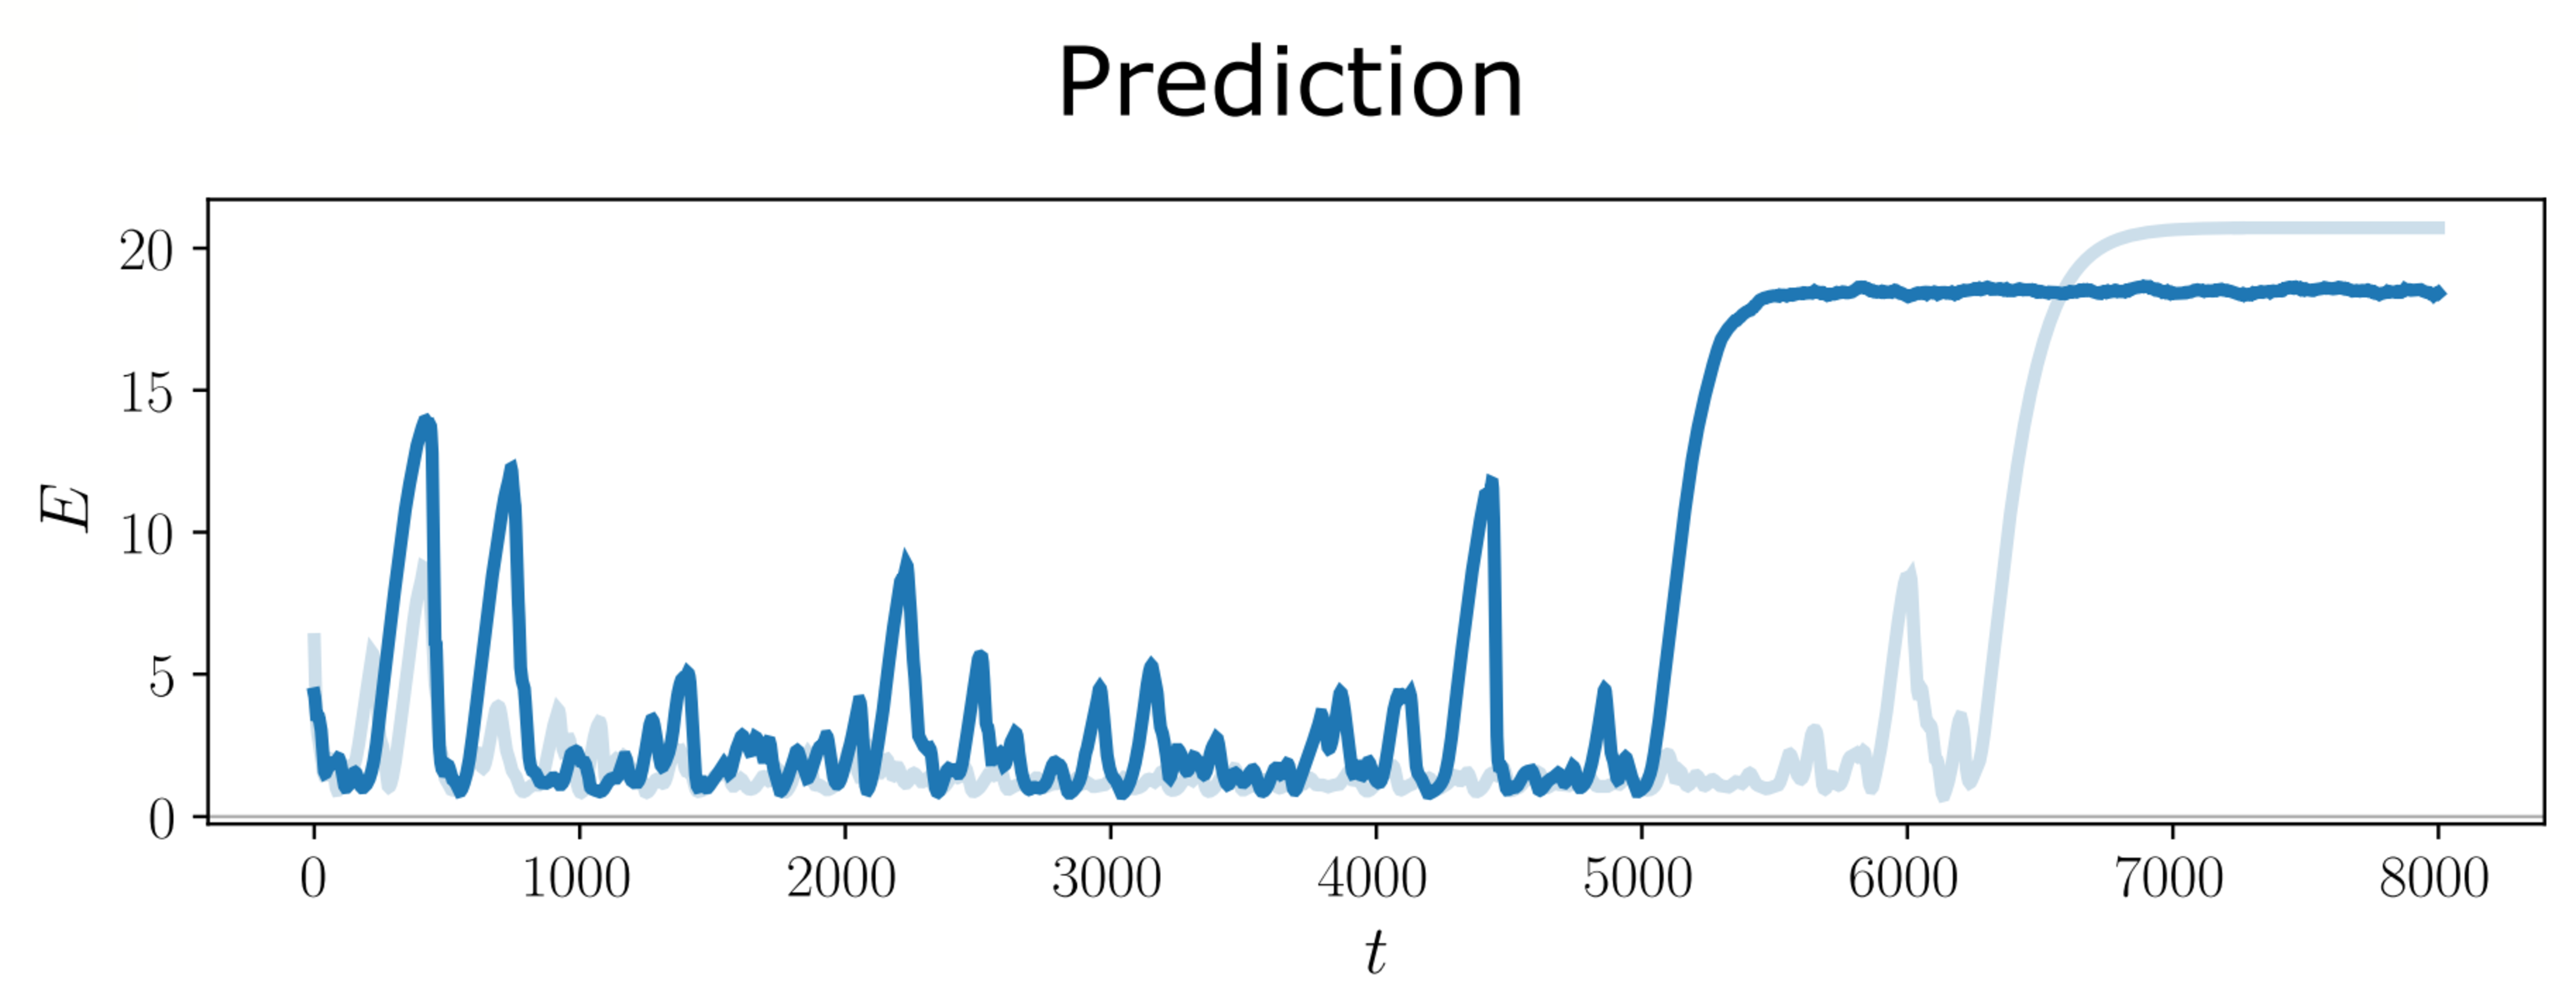
\includegraphics[width = 0.8\textwidth]{figures/prediction/MFE_prediction.pdf}}
%	\subfigure[Re=750 t=780.5]{\includegraphics[width = 1\textwidth]{figures/side_wall/bandwall/band750-106-angle.eps}}
	\end{minipage}
	\quad
	\caption{MFE湍流演化过程中能量随时间变化图。当流场处于湍流状态时能量在较低的范围内波动;流场层流化后流场能量升至某一水平不再变化。图中实线是神经网络预测的MFE流场的能量随时间的变化,虚线是数值模拟MFE流动中能量的变化图。}
\label{fig:MFE}
\end{figure}
\subsection{MFE瞬态性预测方法}
MFE的流动有精确的解析表达,可以被精确表征为9个已知模态的线性组合\cite{Moehlis2004ALM}(式\ref{equ:MFE}),因此任意$t$时刻的流场等价于该时刻各模态对应的9个模数$[a_1(t),a_2(t)...a_9(t)]$。

\begin{equation}\label{equ:MFE}
\begin{aligned}
\bm u(\bm x,t) = \sum_{j=1}^9a_j(t)\bm u_j(\bm x),
\end{aligned}
\end{equation}

每个模态具体数学形式如下:
$$
\bm u_1 =
\begin{bmatrix}
\sqrt{2}sin(\frac{\pi y}{2})\\
0\\
0
\end{bmatrix},
\bm u_2 =
\begin{bmatrix}
\frac{4}{\sqrt{3}}cos^2(\frac{\pi y}{2})cos(\gamma z)\\
0\\
0
\end{bmatrix},
$$

$$
\bm u_3 = \frac{2}{\sqrt{4\gamma^2+\pi^2}}
\begin{bmatrix}
0\\
2\gamma cos(\frac{\pi y}{2})cos(\gamma z)\\
\pi sin(\frac{\pi y}{2})sin(\gamma z)
\end{bmatrix},
\bm u_4 =
\begin{bmatrix}
0\\
0\\
\frac{4}{\sqrt{3}}cos^2(\frac{\pi y}{2})cos(\alpha x)
\end{bmatrix},\\
$$

$$
\bm u_5 =
\begin{bmatrix}
0\\
0\\
2sin(\alpha x)sin(\frac{\pi y}{2})
\end{bmatrix},
\bm u_6 = \frac{4\sqrt{2}}{\sqrt{3(\alpha^2+\gamma^2)}}
\begin{bmatrix}
-\gamma cos(\alpha x)cos^2(\frac{\pi y}{2})sin(\gamma z)\\
0\\
\alpha sin(\alpha x)cos^2(\frac{\pi y}{2})cos(\gamma z)
\end{bmatrix},
$$

$$
\bm u_7 = \frac{2\sqrt{2}}{\sqrt{(\alpha^2+\gamma^2)}}
\begin{bmatrix}
\gamma sin(\alpha x)sin(\frac{\pi y}{2})sin(\gamma z)\\
0\\
\alpha cos(\alpha x)sin(\frac{\pi y}{2})cos(\gamma z)
\end{bmatrix},
\bm u_8 = N_8
\begin{bmatrix}
\pi\alpha sin(\alpha x)sin(\frac{\pi y}{2})sin(\gamma z)\\
2(\alpha^2+\gamma^2)cos(\alpha x)cos(\frac{\pi y}{2})sin(\gamma z)\\
-\pi\gamma cos(\alpha x)sin(\frac{\pi y}{2})cos(\gamma z)
\end{bmatrix},
$$

$$
\bm u_9 = 
\begin{bmatrix}
\sqrt{2}sin(\frac{3\pi y}{2})\\
0\\
0
\end{bmatrix}
$$

由此可以将流场的时间序列精确的压缩为9个模数的时间序列。基于此,Anton等人提出的方法主要思路就是用以上一时刻的流场输入神经网络预测下一时刻,循环的预测后续流场变化。具体地说,将t时刻的9个基础模态对应的模数(即向量$ \bm a(t) =  [a_1(t),a_2(t),...,a_8(t),a_9(t)]^{T}$)输入进神经网络得到$t + \triangle t$时刻的模数$ \bm a(t + \triangle t)$再输入神经网络。循环该过程直到所有训练集数据用完并完成神经网络的训练。Anton等采用的是状态回声网络(Echo State Network,ESN),在其上他们添加了额外的特殊结构以提高网络的泛化性和预测性能。网络的具体结构和参数优化方式参考式\ref{equ:ESN1},\ref{equ:ESN2}。
%\begin{equation}\label{equ:ESN3}
%\begin{aligned}
%\bm W^{T}_{out} = \bm R^{+}A
%\end{aligned}
%\end{equation}
网络训练好后,作者将作为训练集的湍流数据的最后一帧作为原始数据输入到网络中,重复以上一时间步的预测流场作为下一时间步的输入流场循环的预测流场演化过程。作者声称他们训练的网络在多个不同雷诺数下都仅根据湍流时期的数据预测出了MFE流动最终层流化的现象。且他们根据训练好的神经网络在不同雷诺数下进行了多次重复实验得到了不同雷诺数下MFE湍流的寿命分布,与实际寿命分布十分接近。

\begin{figure}[H]
	\subfigbottomskip = 2pt
	\begin{minipage}[h]{0.5\linewidth}
	\centering
	\subfigure[]{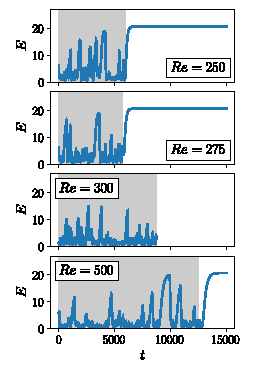
\includegraphics[width = 0.8\textwidth]{figures/prediction/MFE_diffRe.pdf}}
	\end{minipage}
	\quad
	\begin{minipage}[h]{0.5\linewidth}
	\centering
	\subfigure[]{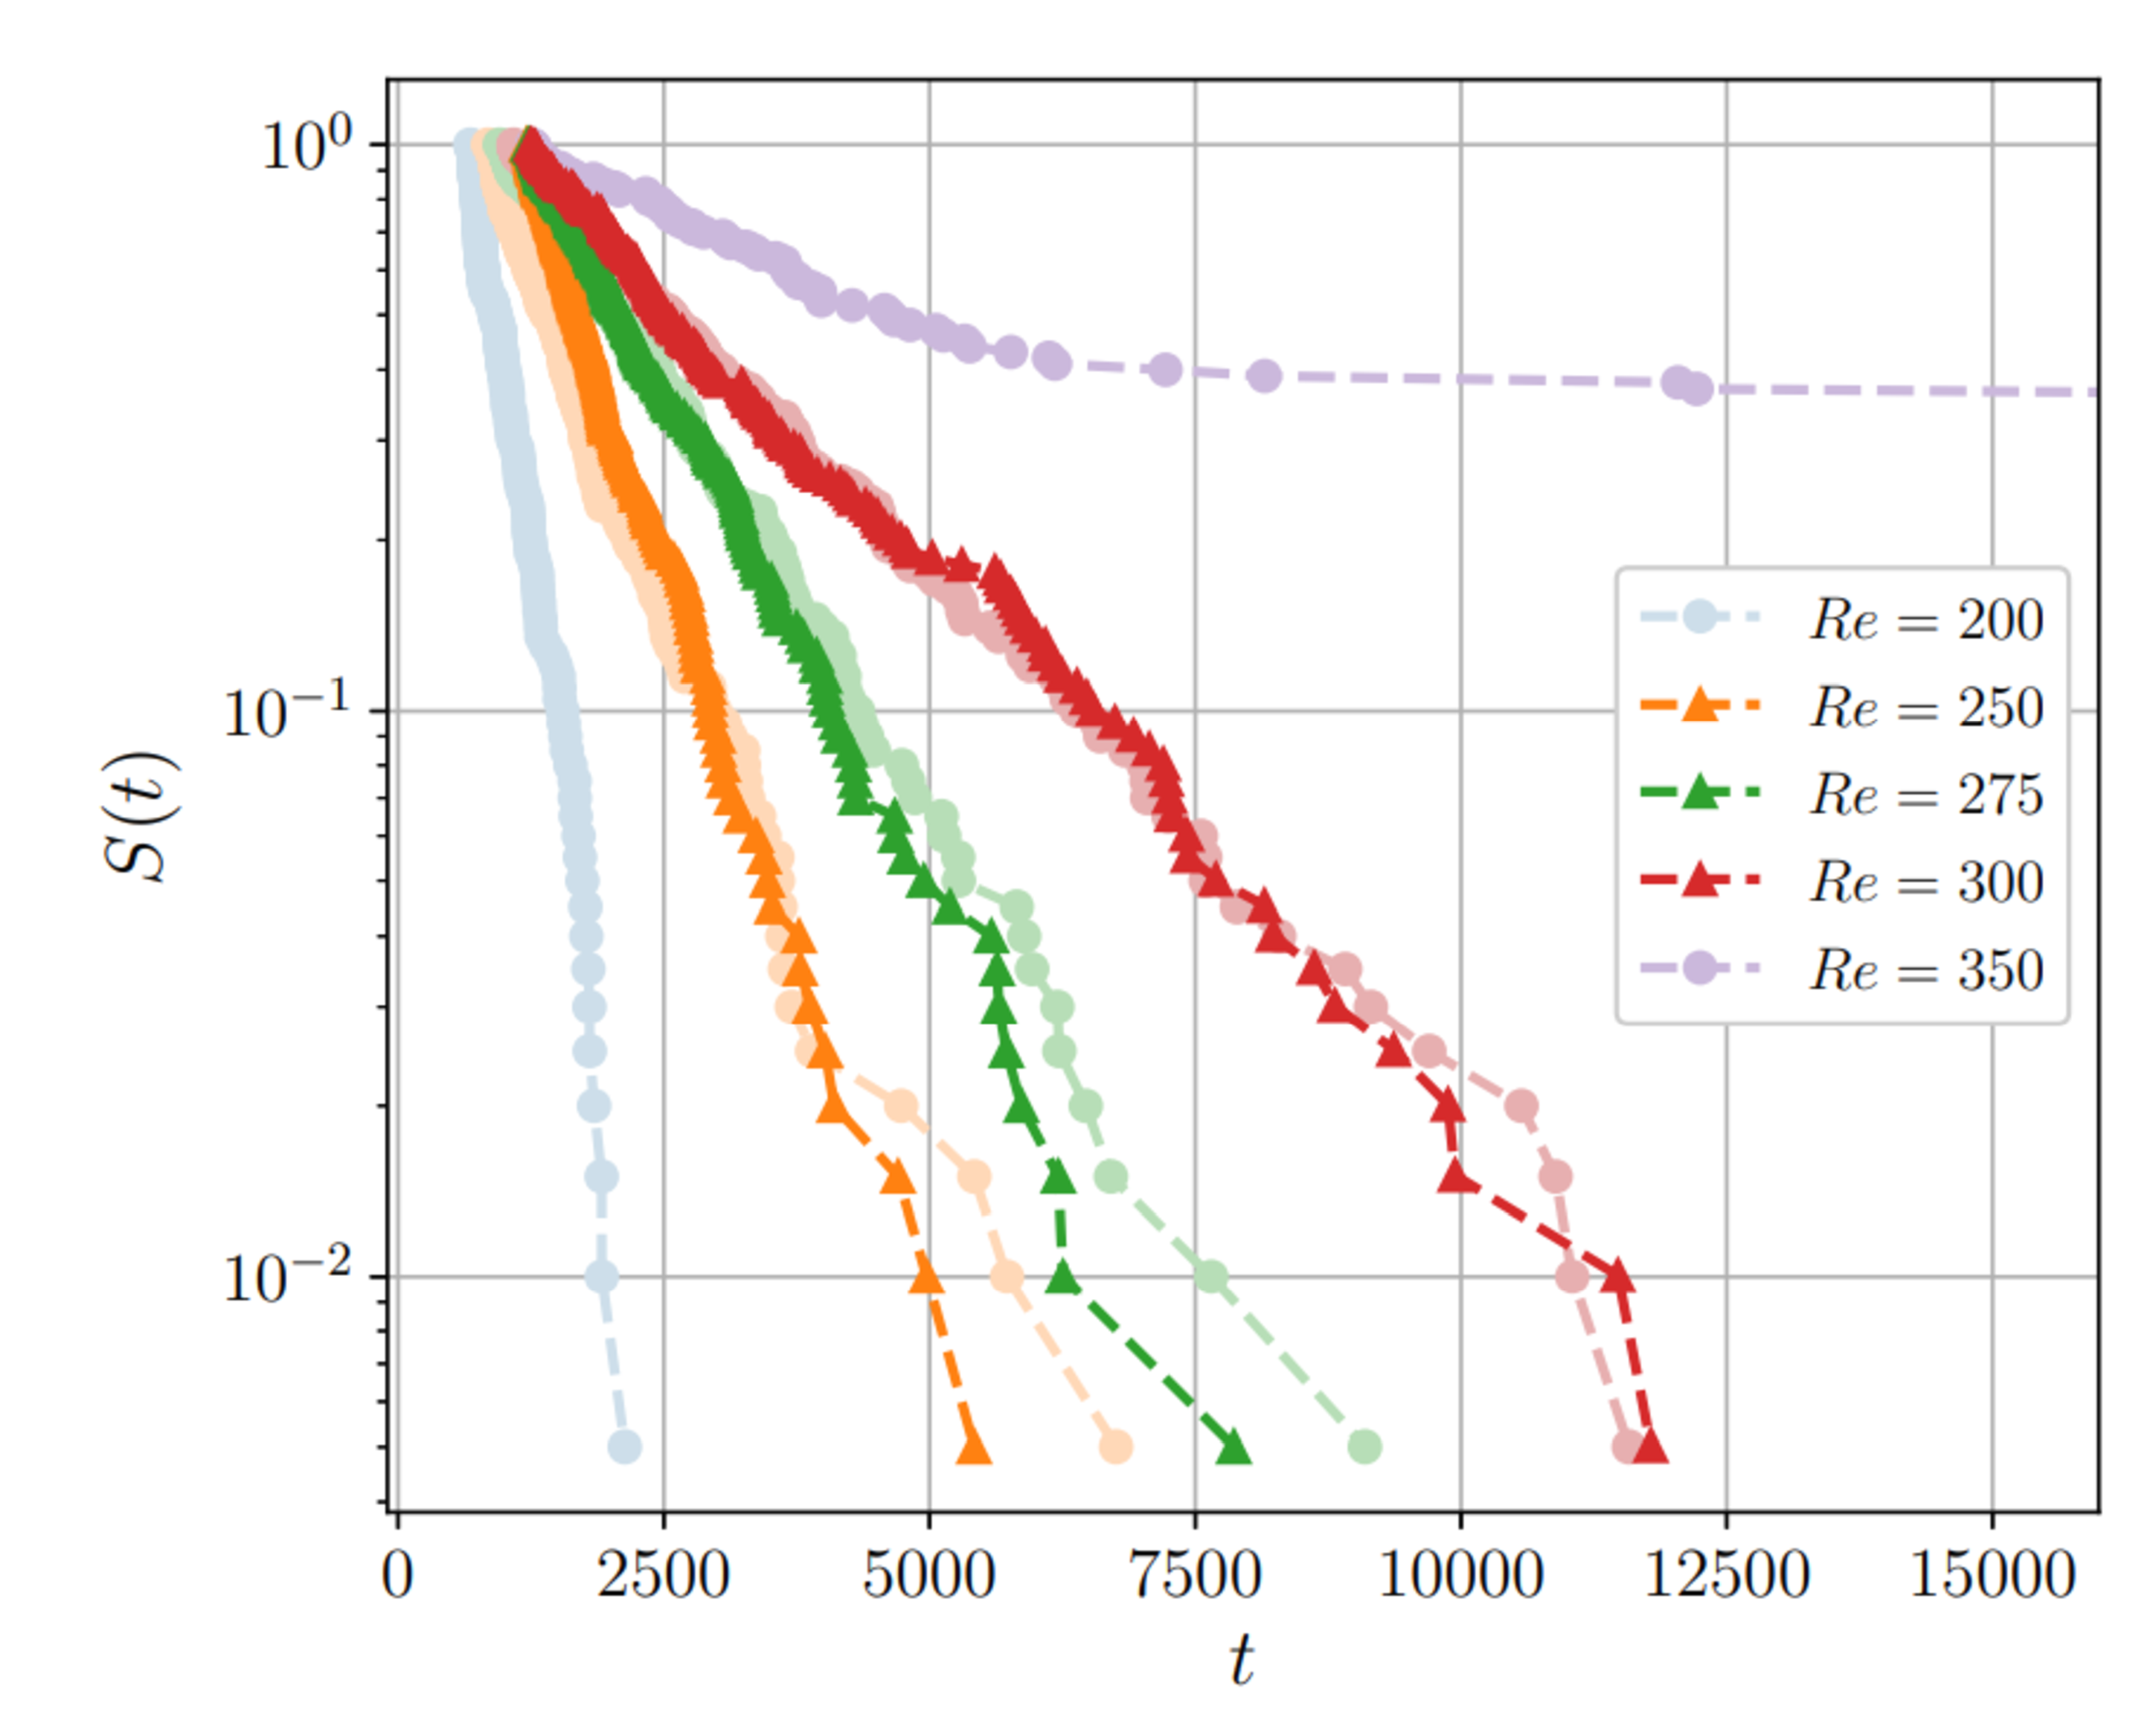
\includegraphics[width = 1.2\textwidth]{figures/prediction/MFE_lifedistri.pdf}}
	\end{minipage}
	\quad
	\caption{(a)不同雷诺数下,通过实际数值计算的流场能量随时间变化图。可以看到在不同雷诺数下,MFE流动的能量最终都会升高到某一值后不再变化(即湍流衰减至层流)。图中阴影部分为用于训练ESN神经网络的湍流数据时间段。(b)MFE湍流的寿命关于雷诺数的分布,横轴是时间纵轴是存活率。其中实线代表神经网络对不同雷诺数下的MFE湍流进行多次重复预测得到的,虚线是实际数值模拟实验得到的寿命分布。}
\label{fig:MFE}
\end{figure}
作者声称他们仅仅根据湍流数据训练的ESN不仅预测出了MFE湍流的层流化,且通过多次重复模拟得到的寿命分布与理论预测高度一致,这说明该方法对于预测非线性力学行为宏观演化趋势有很大的潜力。总结起来该方法可以归纳为以下步骤:

1、获得湍流期流场(模数)时间序列;

2、根据所得时间序列以自回归形式训练神经网络;

3、训练好后的神经网络以自回归形式不断预测后续的流场;

\section{湍流带瞬态性预测}
\subsection{方法迁移}
上一节中提到的预测方法十分简洁直观,有很强的拓展性。但湍流带流场与MFE流场有很大的不同,比如湍流带无法像MFE流动一样给出精确的模态表达且具有更大的复杂性,因此在接下来的章节中将验证该方法迁移到湍流带瞬态性预测任务上的可行性。本文首先通过直接数值模拟获得一段湍流带发展至衰减的时间序列数据,挑选尚未衰减时期的数据通过该方法训练神经网络,考察经过训练的神经网络是否能预测出合理的衰减过程。针对湍流带问题的特殊性本文拟定了如下的训练流程:

1、获得在低雷诺数下单个湍流带衰减至层流状态的完整过程以及其对应的流场时间序列;

2、截取湍流带在衰减前处于湍流时的数据作为训练数据集;

3、用POD方法将流场分解为一系列模态,根据能量累计贡献度截取贡献度高的模态作为主模态以表征湍流带流场。将流场时间序列转化为主模态对应模数的时间序列,即对流场时间序列进行有效的降维压缩;

4、训练神经网络,这里需要注意的是这一步与前面的操作没有强关联,也就是说可以选用不同的,效果更好的神经网络;

5、用训练好的神经网络循环预测湍流带的演化过程,观察是否能预测出衰减现象。

\subsection{湍流带衰减数据}
本文以$Re = 678$下单个湍流带从自持到突然消失的全过程得到的流场时间序列作为原始实验数据,基于此验证该方法的可行性。其中基本流动模型为平板泊肃叶流,在流向和展向上使用周期性边界条件,初始流场中仅有单个湍流带,所采用的数值方法为谱方法\cite{xu_song_2022},基本时间步长为0.025。需要指出的是文中作者求解的是移动坐标系下的NS方程以持续跟踪湍流带的头部区域,并用人工阻尼消去对湍流带在低雷诺数下自持影响不大的尾部部分,故所得的湍流带长度并不及实际湍流带。

整个湍流带在自持了约11602个时间单位后湍流带消失。求解过程中,除了能获得湍流带的流场数据外还同时能获得湍流带头部的运动速度(包括展向,流向)。从图\ref{fig:head_speed}可以看出,在前一段演化时间中,湍流带处于稳定的自持状态,头部展向速度在-0.1附近波动;最后的数百个时间步中,湍流带处于快速衰减状态,可以看到头部展向速度大小快速减小至0。由于变化过大导致计算程序捕捉到的头部速度最后出现了一个不正常的波峰。已有研究表明湍流带头部附近的展向速度型在湍流带自持中扮演了关键角色,因此根据速度时间变化图,拟定将展向速度变化不大的前10000个时间步的流场数据截取作为训练数据训练神经网络,可以合理地认为这段时间内湍流带与自持相关的力学特性变化不大,后面未被截取的数据作为参考组。

值得注意的一点是,Anton在他们的论文中明确提到,训练的MFE流场时间序列中必须包含一段十分接近层流状态的流场,从能量变化图来看就是要有一段能量极高十分接近层流而未达到层流的突变时间段如图\ref{fig:head_speed}。可以观察到在t=9000到t=10000,头部展向速度大小出现突然减小然后又回到-0.1左右。头部运动速度的突变现象一般可以合理地推测头部的非线性稳定性发生了变化,故可合理地认为这两段波动对应的数据即是Anton提及的所谓突变点数据。这也是本文选择这一段时间作为训练数据的原因。
\begin{figure}[H]
	\subfigbottomskip = 2pt
	%\subfigcapskip=-5pt
	\begin{minipage}[h]{\linewidth}
	\centering
	\subfigure{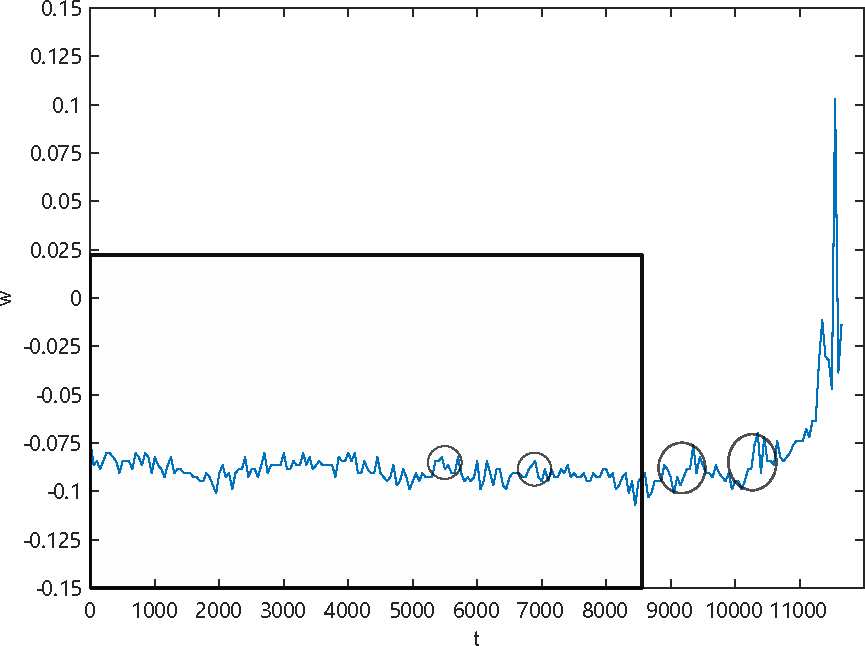
\includegraphics[width =  0.75\textwidth]{figures/prediction/head_speed_pure.pdf}}
%	\subfigure[Re=750 t=780.5]{\includegraphics[width = 1\textwidth]{figures/side_wall/bandwall/band750-106-angle.eps}}
	\end{minipage}
	\quad
	\begin{minipage}[h]{\linewidth}
	\centering
	\subfigure{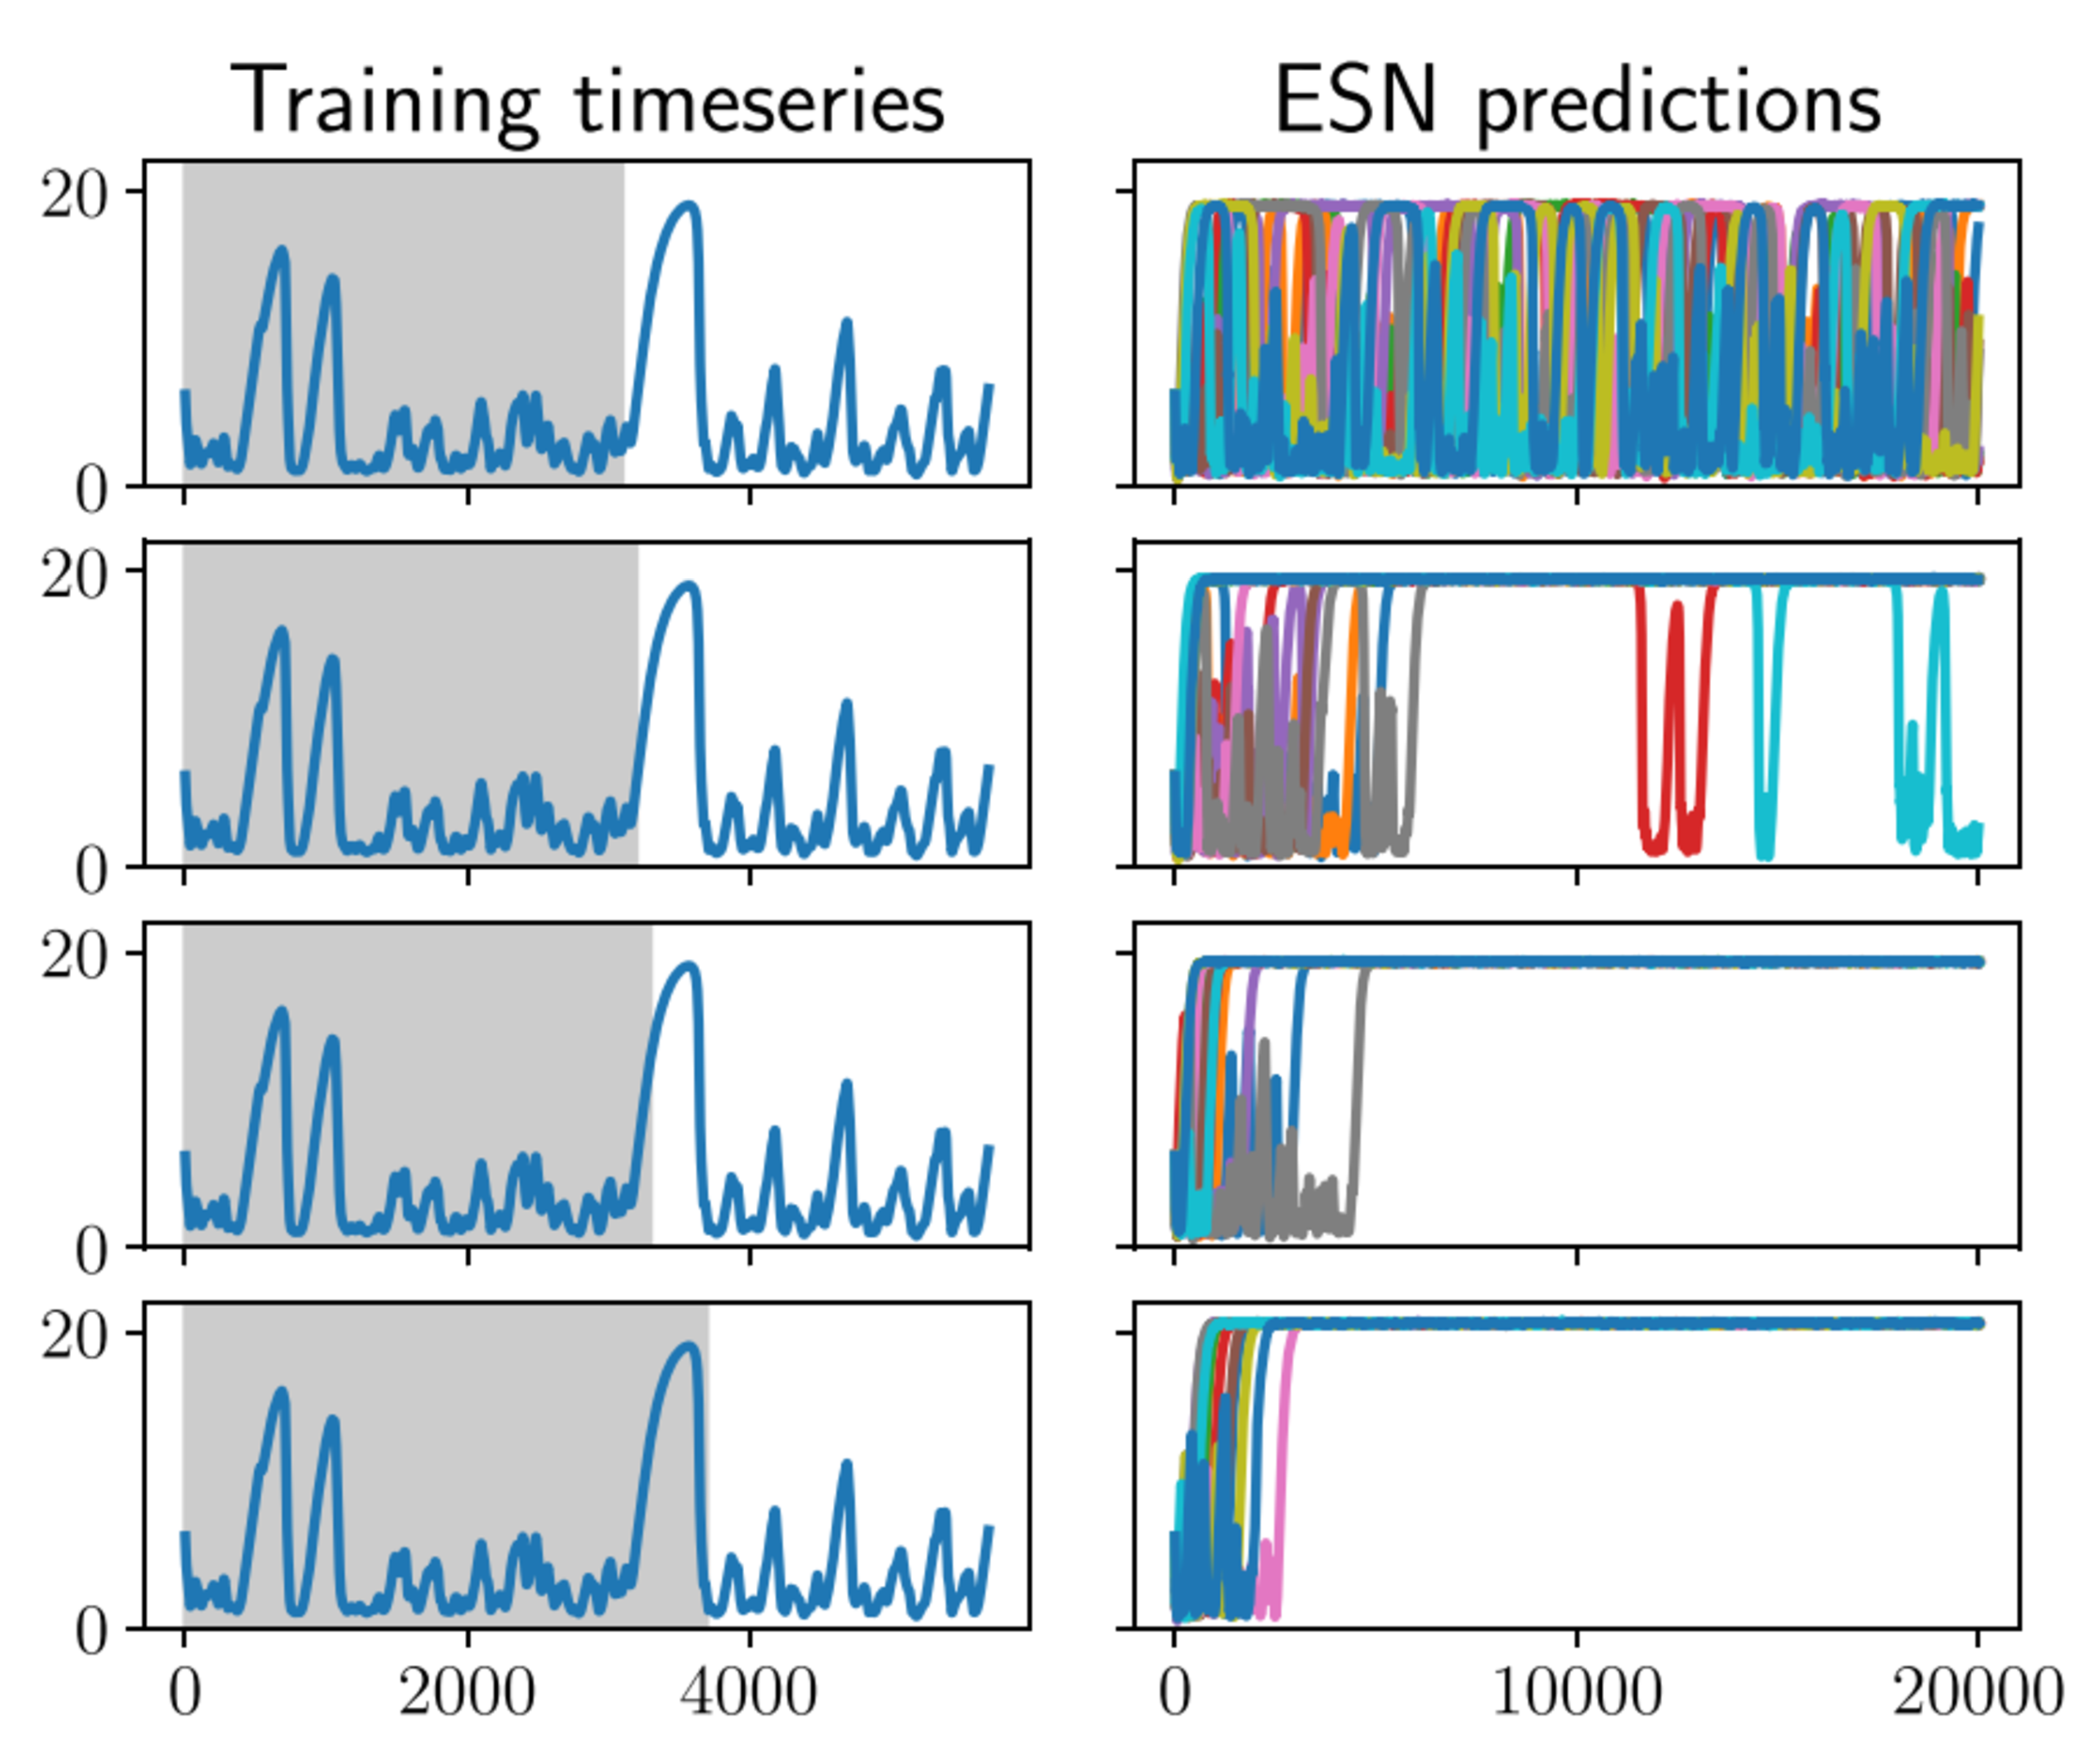
\includegraphics[width =  0.75\textwidth]{figures/prediction/ESN_shock.pdf}}
%	\subfigure[Re=750 t=780.5]{\includegraphics[width = 1\textwidth]{figures/side_wall/bandwall/band750-106-angle.eps}}
	\end{minipage}
	\quad
	\caption{(a)下游头部运动速度展向分量(w)随时间变化图。(b)Anton提到的神经网络因训练数据集不同表现的预测能力的不同,可以看到当训练集没有包含流场十分接近层流态的数据时(能量十分接近层流水平)神经网络无法最终预测出流场的层流化。}
\label{fig:head_speed}
\end{figure}

\subsection{POD模态分解}
获得前10000步的流场作为训练数据后,本文采用经典的POD方法对原始流场作数据压缩处理。POD(Proper Orthogonal Decomposition)是一种将高维数据降维为低维子空间的数学方法。POD的基本思想是通过一系列矩阵运算,将数据集合表示为一组正交基的线性组合,这组基称为“POD模态”。具体来说,POD是将高维数据集合表示为一组正交基的线性组合。这组基包括主模态和副模态。主模态中包括了数据集合的大部分信息,而副模态则主要包含数据集合中的噪声和不规则变化。一个自然的想法是保留包括主要流场信息的主模态,适当舍弃别的副模态。判断主副模态的标准是各个模态对总动能(total kinetic energy,TKE)的贡献度大小。

具体的POD流程如下:设每个流场的数据维度为n(即n个点),流场时间序列长度为m帧,由此第k帧时刻的流场可表示为式\ref{PODdata}。本文研究的是泊肃叶流动中$y = -0.5$上x-z截面流场的展向流速分布。
\begin{equation}
\bm u_k = [u_{k1},u_{k2},...,u_{kn}], k = 1...m\\
\label{PODdata}
\end{equation}

其中n的大小会十分大(与流场中监测点的数量直接相关),例如本文中涉及到的最大的n为$144\times576 = 82944$。根据该时间序列可得一个时间上的平均流场:
\begin{equation}
\overline{\bm u} = \frac{1}{m}\sum_{1}^{m} \bm u_m
\end{equation}

POD的主要降维对象就是时间上的脉动流场$\bm u_m' = \bm u_m - \overline{\bm u}$。为方便表示把所有脉动流场的向量整合为脉动速度矩阵$\bm U$:
$$
\bm U = 
\begin{bmatrix}
\bm u_1'\\
\bm u_2'\\
\bm u_3'\\
\vdots'\\
\bm u_m'
\end{bmatrix}
 = 
\begin{bmatrix}
u_{11}' & u_{12}' & u_{13}' & \cdots u_{1n}'\\
u_{21}' & u_{22}' & u_{23}' & \cdots u_{2n}'\\
u_{31}' & u_{32}' & u_{33}' & \cdots u_{3n}'\\
\vdots\\
u_{m1}' & u_{m2}' & u_{m3}' & \cdots u_{mn}'\\
\end{bmatrix}
\label{PODmat}
$$
此时可以将脉动速度场矩阵和它的转置相乘得到一个对称矩阵:

$$
\bm C = \frac{1}{m-1}\bm U^{T}\bm U =
\begin{bmatrix}
\frac{1}{m-1}\sum_{i=1}^{m}{u_{i1}'}^2 & \cdots \\
\vdots & \frac{1}{m-1}\sum_{i=1}^{m}{u_{i2}'}^2 & \cdots & \cdots \cdots\\
\vdots & \cdots & \frac{1}{m-1}\sum_{i=1}^{m}{u_{i3}'}^2 & \cdots \cdots\\
\vdots & \vdots\\
\vdots & \cdots & \cdots & \cdots \frac{1}{m-1}\sum_{i=1}^{m}{u_{in}'}^2\\
\end{bmatrix}
\label{PODeny}
$$

\begin{equation}
TKE = \frac{1}{n}\sum_{i=1}^{n}\frac{1}{m-1}\sum_{j=1}^{m}{u_{ij}'}^2
\label{equ:TKE}
\end{equation}
得到的$\bm C^{n\times n}$对角线上每一项对应的都是某一点处时间上的脉动动能平均,对角线之外的项从统计的角度上来说属于不同变量之间的协方差。从物理的角度来说,矩阵$\bm C$的迹即为总体动能(total kinetic energy,TKE,参考式\ref{equ:TKE})。从能量的角度看,如果所有流场都能被分解成一系列模态的叠加,我们会希望能知道哪些模态对TKE的贡献更大哪些影响较小,保留贡献大的模态(主模态)舍弃贡献小的模态(副模态)以达到降维的目的。但其中协方差项裹挟了不同模态在能量上的信息干扰了主要模态的分析,因此会希望能将流场分解为一系列正交的模态以使得在求TKE时协方差项为0,从而很好的分辨各个模态的能量贡献度。对$\bm C$做正交变换得$\bm C = \Phi\Lambda\Phi^{T}$。其中$\bm \Phi$即为所求得的正交模态,将脉动速度矩阵$\bm U$与正交阵$\bm \Phi$相乘可得到各个时刻流场模态分解对应的模数$\bm A$,即:

$$\bm A^{m\times n} = \bm U^{m\times n}\Phi^{n\times n}$$

可以看出$\bm A$的数据大小与$\bm U$一致尚未达到数据降维的目的。但这里需要指出的是,A本身与自身转置相乘后得到的是对角阵$\Lambda$(没有协方差项干扰),且该对角阵忠实的保留了$\bm U$的TKE信息:

%\begin{align}
%a + b\\
%c + d
%\end{align}
\begin{align}
\frac{1}{m-1}\bm A^{T}\bm A = \frac{1}{m-1}(\bm U\bm \Phi)^{T}(\bm U\bm \Phi)\notag \\
= \frac{1}{m-1}(\bm \Phi^{T}\bm U^{T}\bm U\bm \Phi)\notag \\
=\bm\Phi^{T}\bm C\bm \Phi = \bm\Phi^{T}\bm\Phi\Lambda\Phi^{T}\bm \Phi\notag \\ 
= \bm \Lambda = 
\begin{bmatrix}
\lambda_{1} &   & &  &\\
	  & \lambda_{2} &  & &\\
	  &   & \lambda_{3}& &\\
	  &   &  \ddots &  &\\
	  &   &   &     \lambda_{n}   &
\end{bmatrix}
\end{align}

$$
tr(\bm \Lambda) = TKE(\bm U)
$$

$\bm \Lambda$中对角线上的每一项特征值$\lambda_{i}$代表了对应模态对TKE贡献的绝对大小,特征值越大对TKE的贡献越大。为统一标准一般考虑的是各模态对TKE贡献的百分比,即$\frac{\lambda_{i}}{\sum_{j=1}^{n}\lambda_{j}}$。因此可以把特征值从大到小排列,只保留前面一定数量的模态保证这些模态的和对TKE贡献度大于某个阈值(如90\%),而对于靠后的贡献较小的模态可直接舍弃以达到降维的目的。
%\begin{figure}[htb]
%	\subfigbottomskip = 2pt
%	%\subfigcapskip=-5pt
%	\begin{minipage}[h]{\linewidth}
%	\centering
%	\subfigure{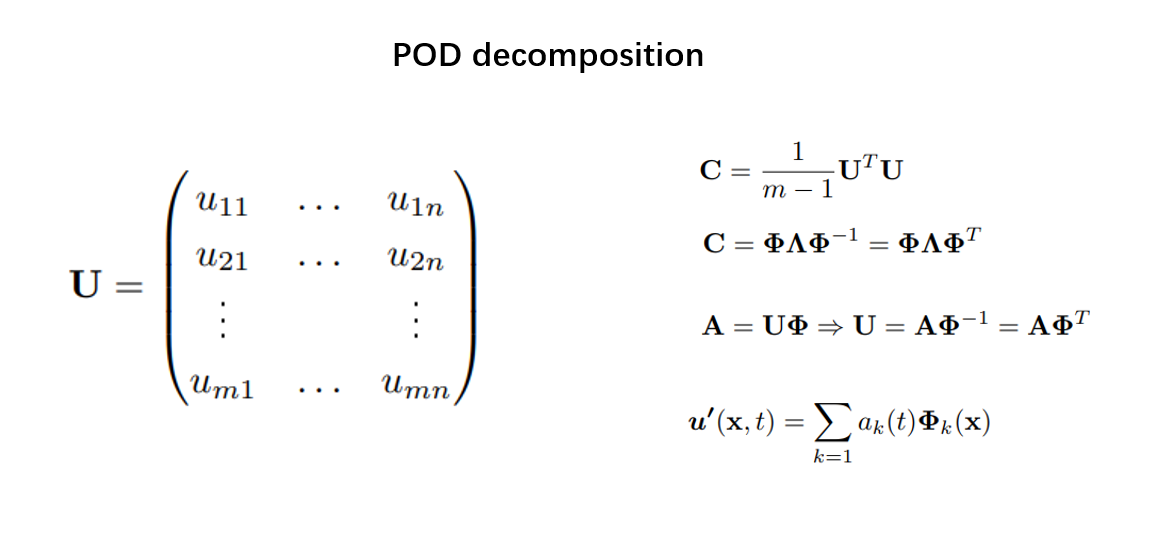
\includegraphics[width = \textwidth]{figures/prediction/POD_procedure.png}}
%	\end{minipage}
%	\quad
%	\caption{POD的具体过程}
%\label{fig:pod}
%\end{figure}

通过以上步骤对Re=678的数据进行POD处理后可得到一系列的模态,图\ref{fig:main_mode_sample}列举了前几个主要模态的速度分布,接下来就是要截断副模态保留主模态。一般以$90\%$为基准判定主副模态,图\ref{fig:main_mode} 展示了原始数据中模态的累计贡献度,可以看出在第150个模数时,占比约为$90\%$。故选择前150个模态的模数作为ESN网络的输入。
\begin{figure}[htb]
	\subfigbottomskip = 2pt
	\begin{minipage}[h]{0.33\linewidth}
	\centering
	\subfigure[mode = 1]{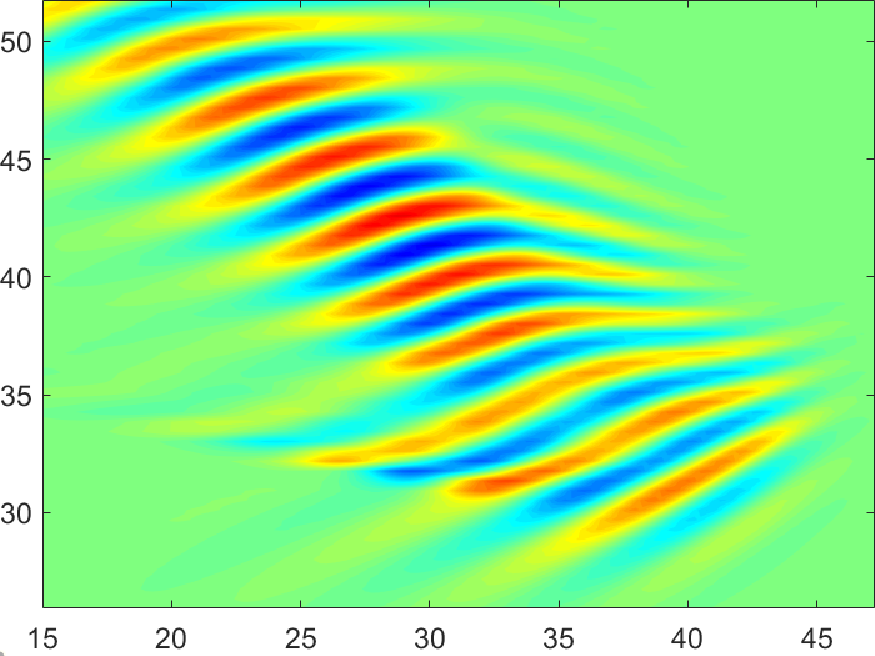
\includegraphics[width = \textwidth]{figures/prediction/mode1.pdf}}
	\end{minipage}
	\begin{minipage}[h]{0.33\linewidth}
	\centering
	\subfigure[mode = 2]{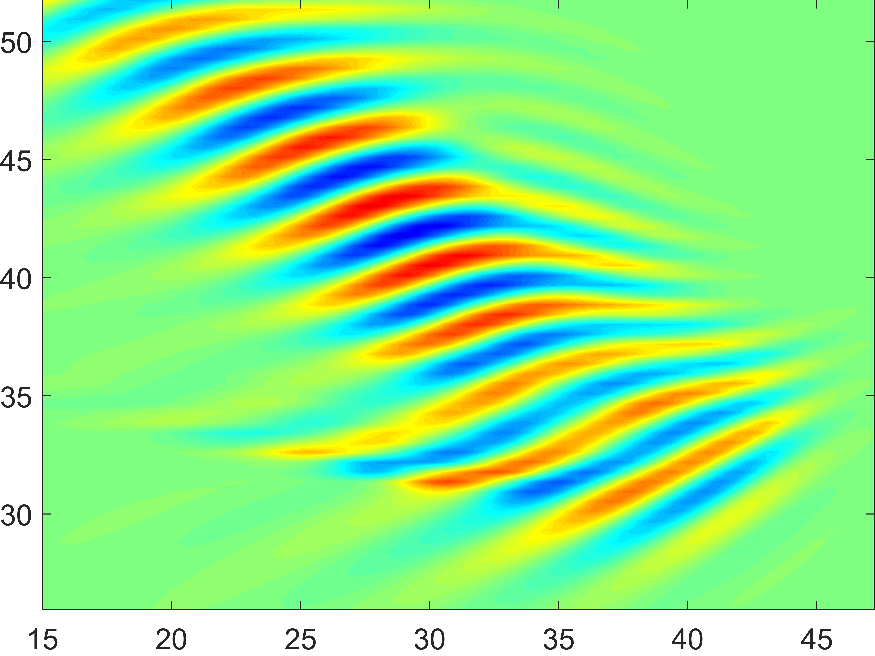
\includegraphics[width = \textwidth]{figures/prediction/mode2.pdf}}
	\end{minipage}
	\begin{minipage}[h]{0.33\linewidth}
	\centering
	\subfigure[mode = 3]{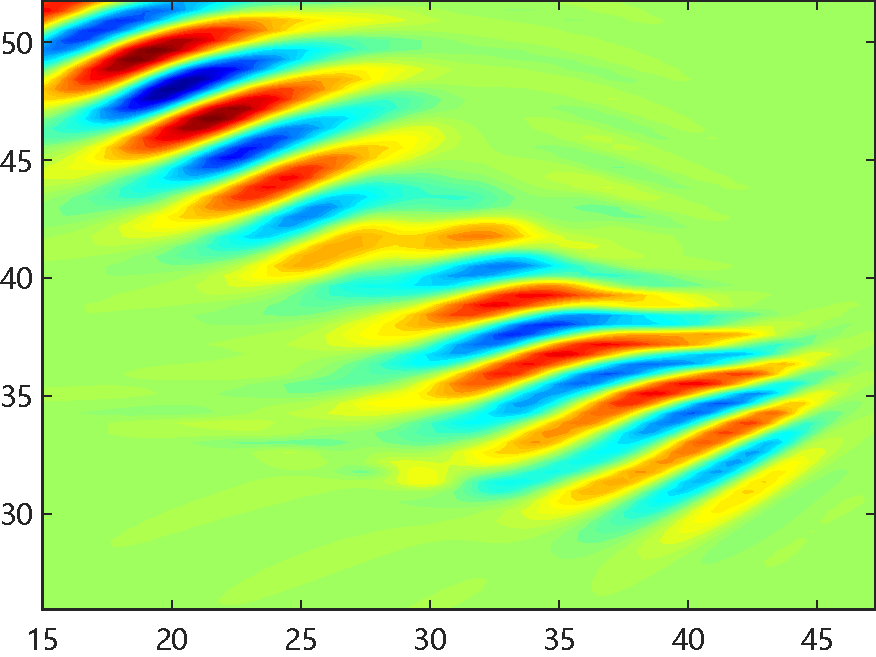
\includegraphics[width = \textwidth]{figures/prediction/mode3.pdf}}
	\end{minipage}
	\caption{POD处理后得到的前三个个主要模态。}
\label{fig:main_mode_sample}
\end{figure}

\begin{figure}[H]
	\subfigbottomskip = 2pt
	%\subfigcapskip=-5pt
	\begin{minipage}[h]{\linewidth}
	\centering
	\subfigure{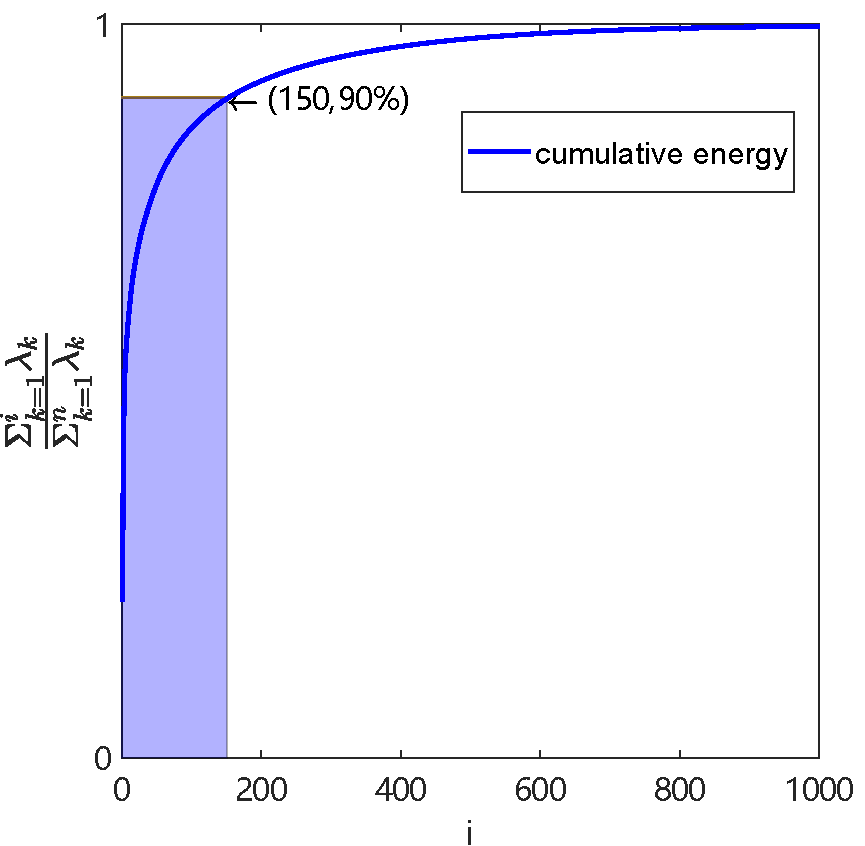
\includegraphics[width = 0.5\textwidth]{figures/prediction/lamcum.pdf}}
%	\subfigure[Re=750 t=780.5]{\includegraphics[width = 1\textwidth]{figures/side_wall/bandwall/band750-106-angle.eps}}
	\end{minipage}
	\quad
	\caption{主要模态对方差的累计贡献的百分比图,为方便展示此处仅列出前1000个模数对应的特征值。}
\label{fig:main_mode}
\end{figure}

\subsection{神经网络训练与预测}
\subsubsection{ESN 网络}
依上述步骤对数据预处理后开始训练网络,首先本文尝试了Anton等提出的ESN网络。和别的RNN类网络一样ESN网络通过隐藏层状态(ESN中称为池化层)传递历史信息以供网络预测未来的状态。具体训练过程如图\ref{fig:ESN_structure},将上一个时刻预测得到的流场模数$\bm a(t)$和隐藏层状态$\bm r(t)$输入网络预测下一个时刻的流场$\bm a(t+\triangle t)$以及池化层状态$\bm r(t+\triangle t)$,再输入ESN预测再下一个时刻循环往复。对应的数学表达式如式(\ref{equ:ESN1}),(\ref{equ:ESN2})所示。
\ref{fig:ESN_structure})。
\begin{figure}[H]
	\subfigbottomskip = 2pt
	\begin{minipage}[h]{\linewidth}
	\centering
	\subfigure{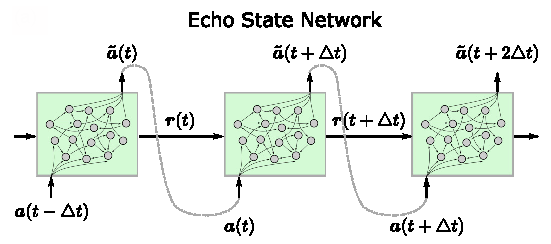
\includegraphics[width = 0.9\textwidth]{figures/prediction/ESN_structure.pdf}}
	\end{minipage}
	\quad
	\caption{ESN网络训练预测示意图。$\bm a(t)$为t时刻流场的模数,$\bm r(t)$为该时刻池化层的状态。}
\label{fig:ESN_structure}
\end{figure}

\begin{equation}\label{equ:ESN1}
\begin{aligned}
\bm r(t+\triangle t) = tanh[\bm b + \bm W\bm r(t) + \bm W_{in}\bm a(t)] + \xi \bm Z
\end{aligned}
\end{equation}
\begin{equation}\label{equ:ESN2}
\begin{aligned}
\underset{W_{out}}{min} \sum_{k=1}^{N_t} \Vert \bm W_{out} \bm r(k\triangle t) -\bm a(k\triangle t) \Vert^{2}_{2},
\end{aligned}
\end{equation}

\begin{equation}
\begin{aligned}
\bm W^{T}_{out} = (\bm R^{T} \bm R)^{-1}\bm R^{T}\bm A,
\end{aligned}\label{equ:ESN3}
\end{equation}

式(\ref{equ:ESN1})称为池化计算,$\bm r$为池化层。池化层中的$\bm b$为偏置向量,$\bm W$为池化层矩阵,$\bm W_{in}$为输入矩阵,这些参数仅在初始时随机初始化确定,后续训练学习过程中不再改变;$\bm Z$为一[0,1]上随机向量,$\xi$是一固定常数用以控制随机向量大小。原文中作者特别指出,他们特别添加的该项随机扰动项能使ESN网络具有更好的泛化性和预测能力。ESN网络中需要训练改变的参数仅为式(\ref{equ:ESN2})中的输出矩阵$\bm W_{out}$。由于优化参数仅涉及一个线性变换矩阵$\bm W_{out}$,因此ESN的训练过程仅需式(\ref{equ:ESN3})一步即可将误差降至理论上最优,其中矩阵$\bm A$为时间序列组成的矩阵$[\bm a(\triangle t),\bm a(2\triangle t), ...\bm a(N_{t}\triangle t)]$,$\bm R$为对应的隐藏层时间序列$[\bm r(\triangle t),\bm r(2\triangle t), ...\bm r(N_{t}\triangle t)]$组成的矩阵。极少的参数意味着训练过程所需要的计算资源和计算时间极少,因此相较其它结构复杂的神经网络,ESN可以一次输入所有训练数据并给出全局误差最小的解。

ESN的超参数主要有4个:池化层矩阵$\bm W$的维度$N_{r}$,池化层矩阵的谱半径$\rho$,决定池化层内部链接程度的稀疏度$s$以及控制随机因子大小的$\xi$。其中设置$\xi = 10^{-3}$。由于此时的输入维度远高于\cite{Anton2023}中的9个,故其它超参数的确定主要参考\cite{Pandey2020}给出的数据。\cite{Pandey2020}中采用了相似的先根据POD得出主模态表征流场再用ESN预测流动的方法,且使用的POD模数恰好也为150。该文作者通过多次实验微调给出了输入维度150时,最优的池化层维度应为$N_{r}=2100$并给出了此时其它超参数$\rho$,$s$的最优组合。为了考察该组超参数组合是否适合本文采用的ESN网络,故做了一系列对照实验以确定最优的$N_{r}$。将10000步湍流数据划分成前80\%作为测试集,后20\%作为验证集测试了6个不同的$N_{r}$下ESN网络的表现。如表\ref{tab:hyper_parameter}所示,在控制其它超参数保持为默认值不变的情况下,分别实验了不同大小池化层在训练数据集上的表现。比较训练误差和验证误差可以看出随着池化层规模的增大训练误差在不断减小,这是由ESN的结构决定的;然而验证集误差在$N_{r} = 3000$时取得最小。因此可以确定本文采用的ESN网络的最优池化层大小应为$N_{r} = 3000$。考虑到文中的150个模态对应的能量贡献度仅为$83\%$低于本文的$90\%$,故可以合理地认为本文采用的模型与\cite{Pandey2020}中的模型相似,故采取相同的超参数组合(表\ref{tab:optim_parameter})。

\begin{table}
\centering
\begin{tabular}{c|c|c|c}
\textbf{$N_{r}$} & \textbf{Train error} & \textbf{validation error} & \textbf{time}\\
\hline
750  & 0.00901 & 0.0258 & 31.1\\
1500 & 0.00412 & 0.0165 & 31.9\\
2100 & 0.00270 & 0.0142 & 59.6\\
2400 & 0.00227 & 0.0139 & 77.9\\
3000 & 0.00162 & 0.0131 & 79.6\\
5000 & 0.00061 & 0.0135 & 358.2\\
\end{tabular}
\label{tab:hyper_parameter}
\caption{不同池化层大小下ESN网络的表现。}
\end{table}

\begin{table}
\centering
\begin{tabular}{c|c|c|c}
\textbf{$N_{r}$} & \textbf{$\xi$} & \textbf{$\rho$} & \textbf{$s$}\\
\hline
3000 & 0.001 & 0.95 & 0.8 \\
\end{tabular}
\caption{\label{tab:optim_parameter}本文中ESN采用的超参数组合}
\end{table}

从流场能量的角度看,ESN在训练集上的拟合很好(图\ref{fig:esn_perform}(a)),预测流场与实际流场的能量几乎一致,这得益于它全局优化的训练算法。随后使训练好后的ESN向后继续预测了4000个时间步,ESN预测的后续流场能量快速衰减到很低的水平(图\ref{fig:esn_perform}(b)),这与数值模拟中湍流带正常衰减过程中能量的变化十分相似。

\begin{figure}[H]
	\subfigbottomskip = 2pt
	%\subfigcapskip=-5pt
	\begin{minipage}[h]{\linewidth}
	\subfigure[]{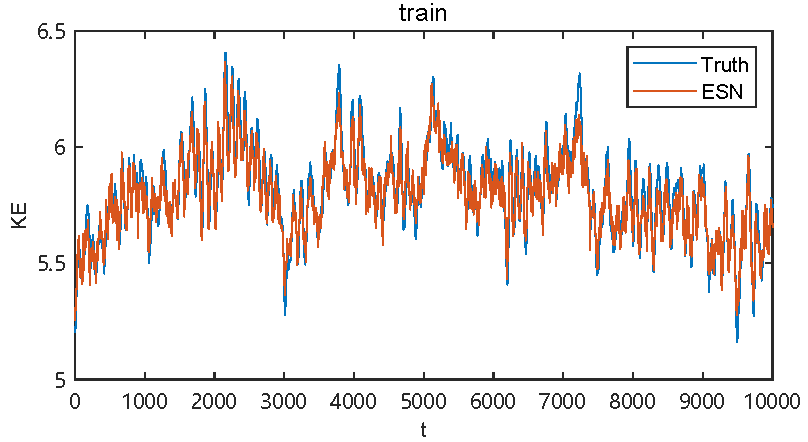
\includegraphics[width = \textwidth]{figures/prediction/traincomp.pdf}}
	\end{minipage}
	\quad
	\begin{minipage}[h]{\linewidth}
	\subfigure[]{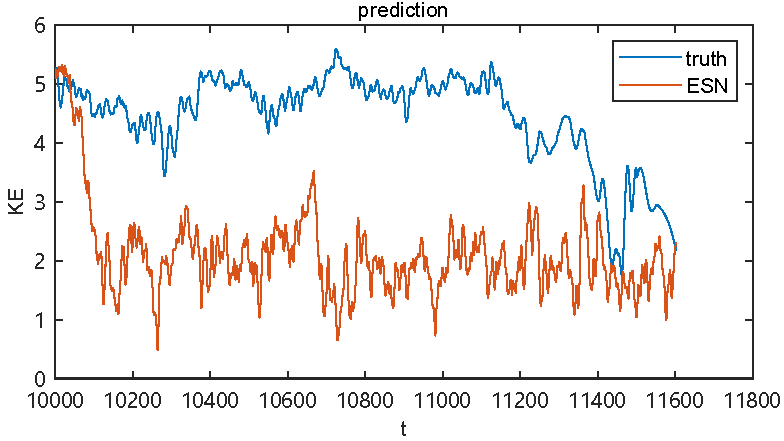
\includegraphics[width = \textwidth]{figures/prediction/energycomp.pdf}}
	\end{minipage}
	\quad
%	\begin{minipage}[h]{0.5\linewidth}
%	\centering
%	\subfigure[]{\includegraphics[width = \textwidth]{figures/prediction/esn_pred.png}}
%%	\subfigure[Re=750 t=780.5]{\includegraphics[width = 1\textwidth]{figures/side_wall/bandwall/band750-106-angle.eps}}
%	\end{minipage}
%	\quad
	\caption{(a)在训练数据集中ESN预测的流场的流场能量与实际流场的能量对比。(b)ESN向后预测的流场能量与实际能量对比。}
\label{fig:esn_perform}
\end{figure}

但是从ESN预测的衰减过程和实际衰减过程(图\ref{fig:esn_decay})来看,ESN预测的衰减流场丢失了许多重要的力学特征,比如衰减时可以观察到条纹角度大小连续平缓的减小,湍流带头部速度强度的逐渐降低,湍流带本身速度条纹的减弱。因此可以认为,虽然ESN预测出了整体的衰减,但是它并没有能捕捉到演化过程中关键的力学特征,这说明它得到的结果是非物理、可参考性极低的。
\begin{figure}[H]
	\subfigbottomskip = 2pt
	%\subfigcapskip=-5pt
	\begin{minipage}[h]{0.22\linewidth}
	\centering
	\subfigure[Truth t=10001]{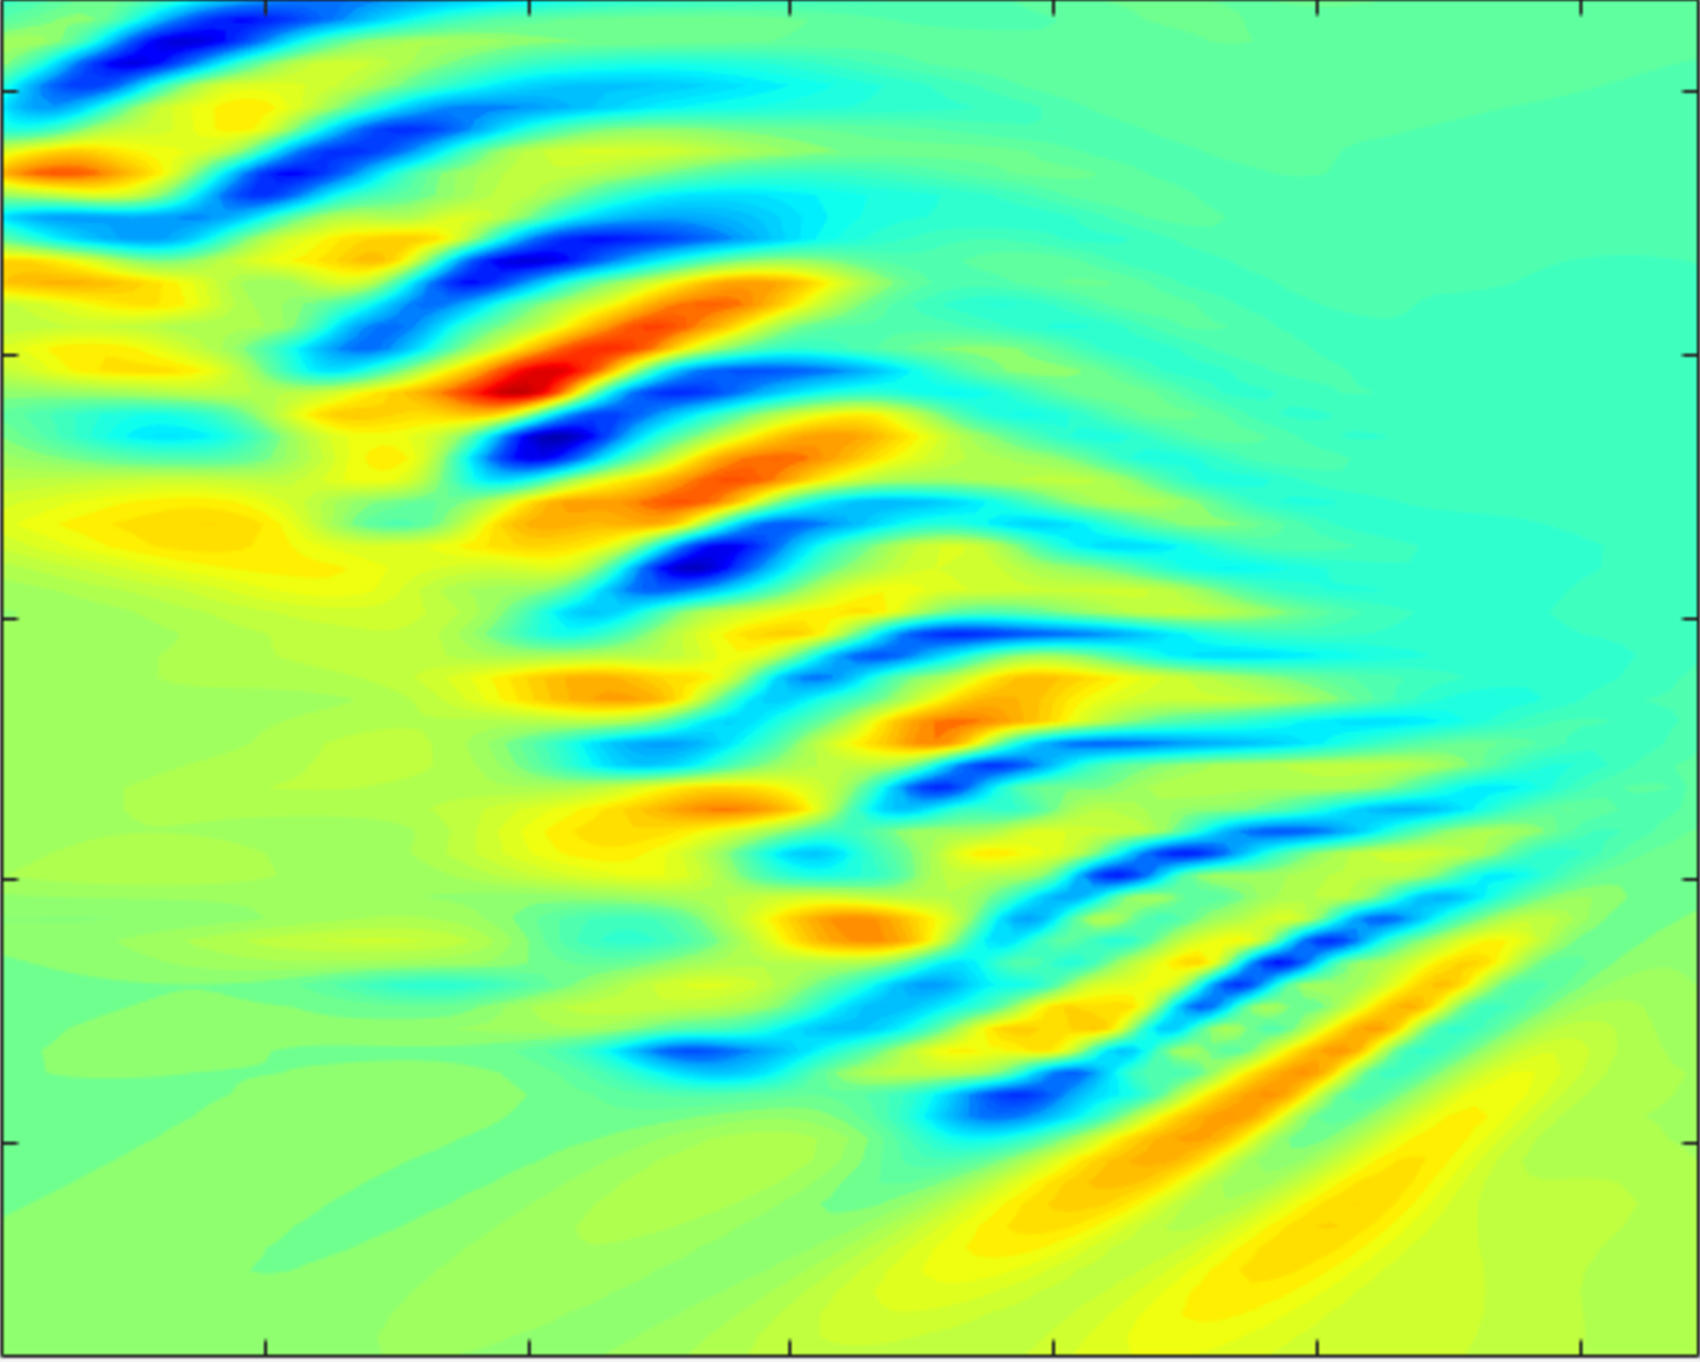
\includegraphics[width = \textwidth]{figures/prediction/actual4001.pdf}}
	\end{minipage}
	\quad
	\begin{minipage}[h]{0.22\linewidth}
	\centering
	\subfigure[t=10050]{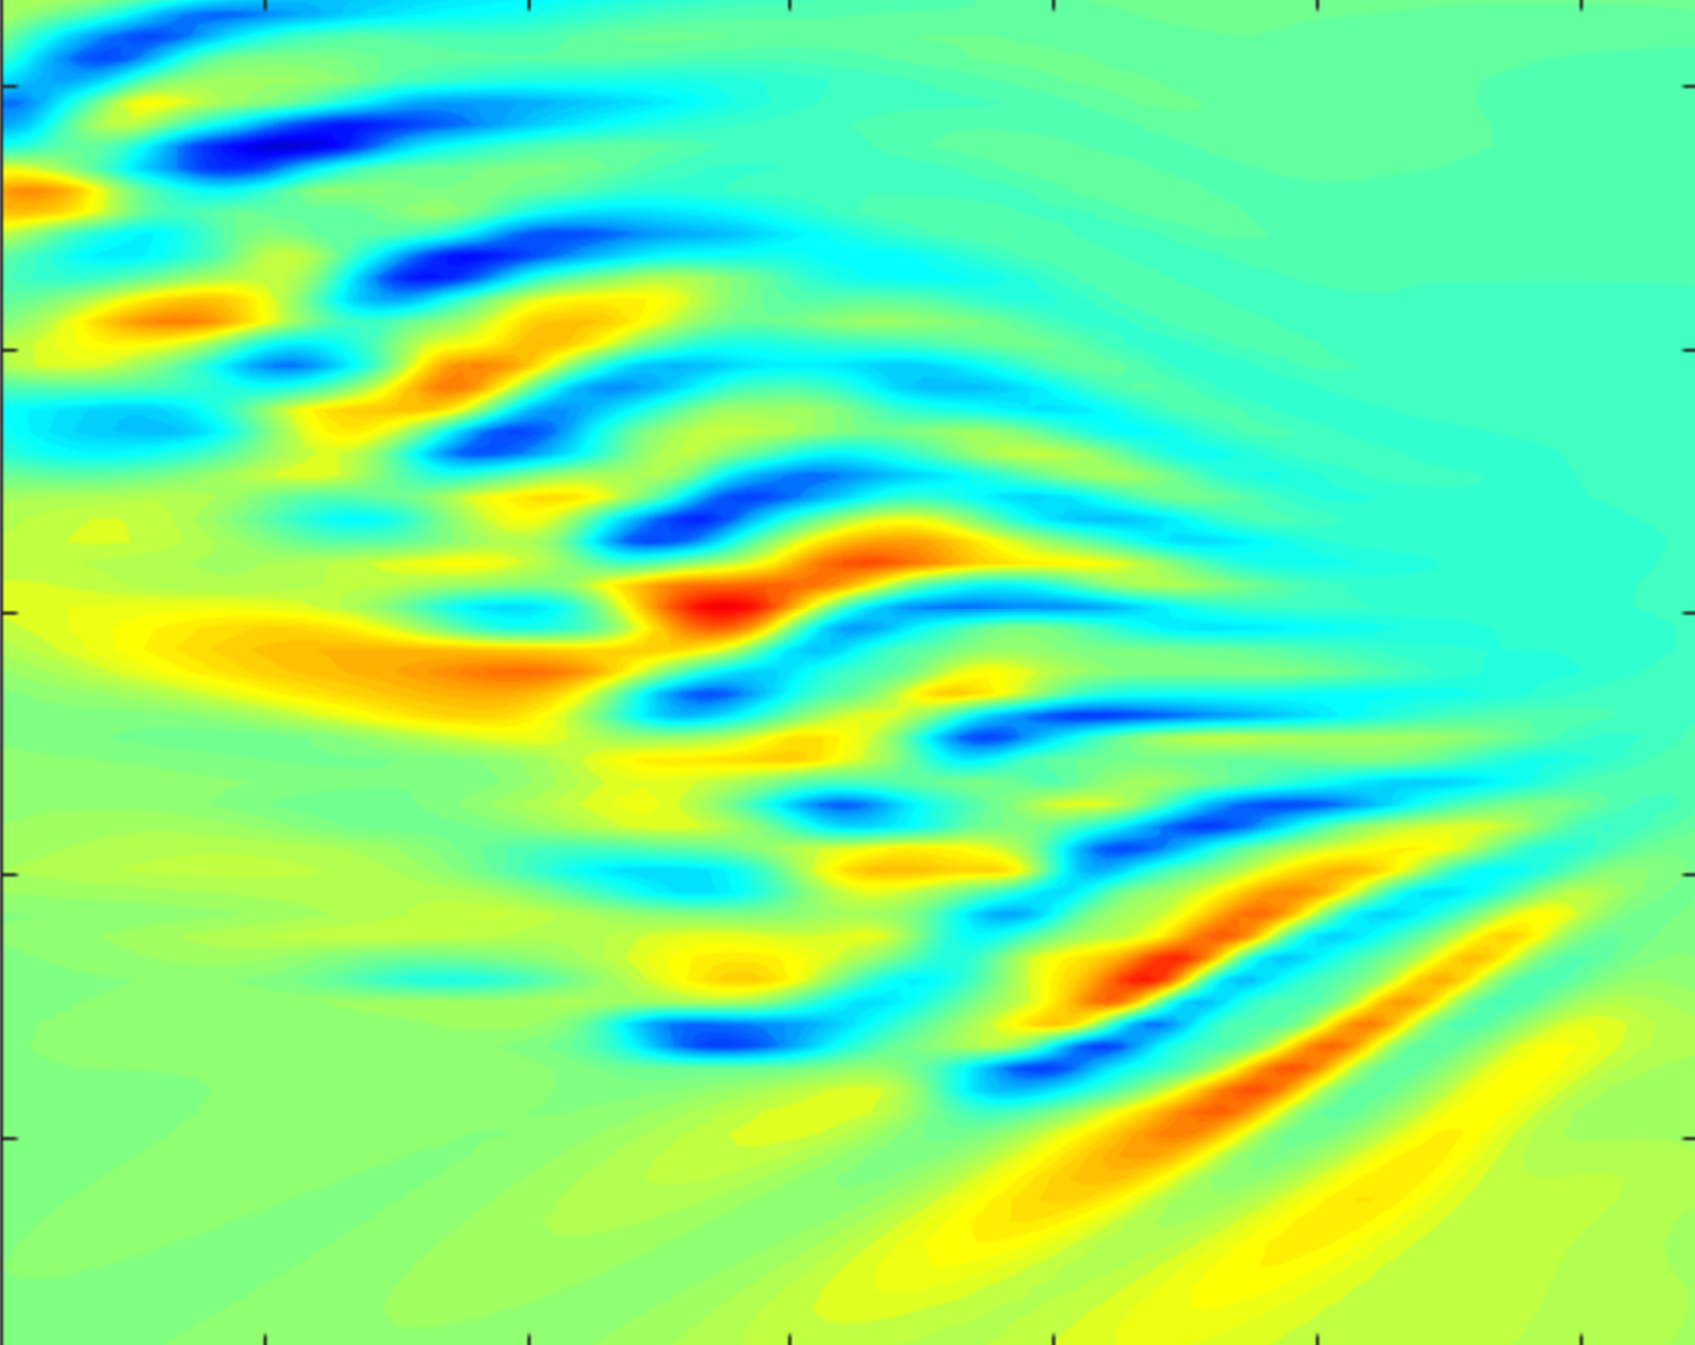
\includegraphics[width = \textwidth]{figures/prediction/actual4250.pdf}}
	\end{minipage}
	\quad
	\begin{minipage}[h]{0.22\linewidth}
	\centering
	\subfigure[t=10250]{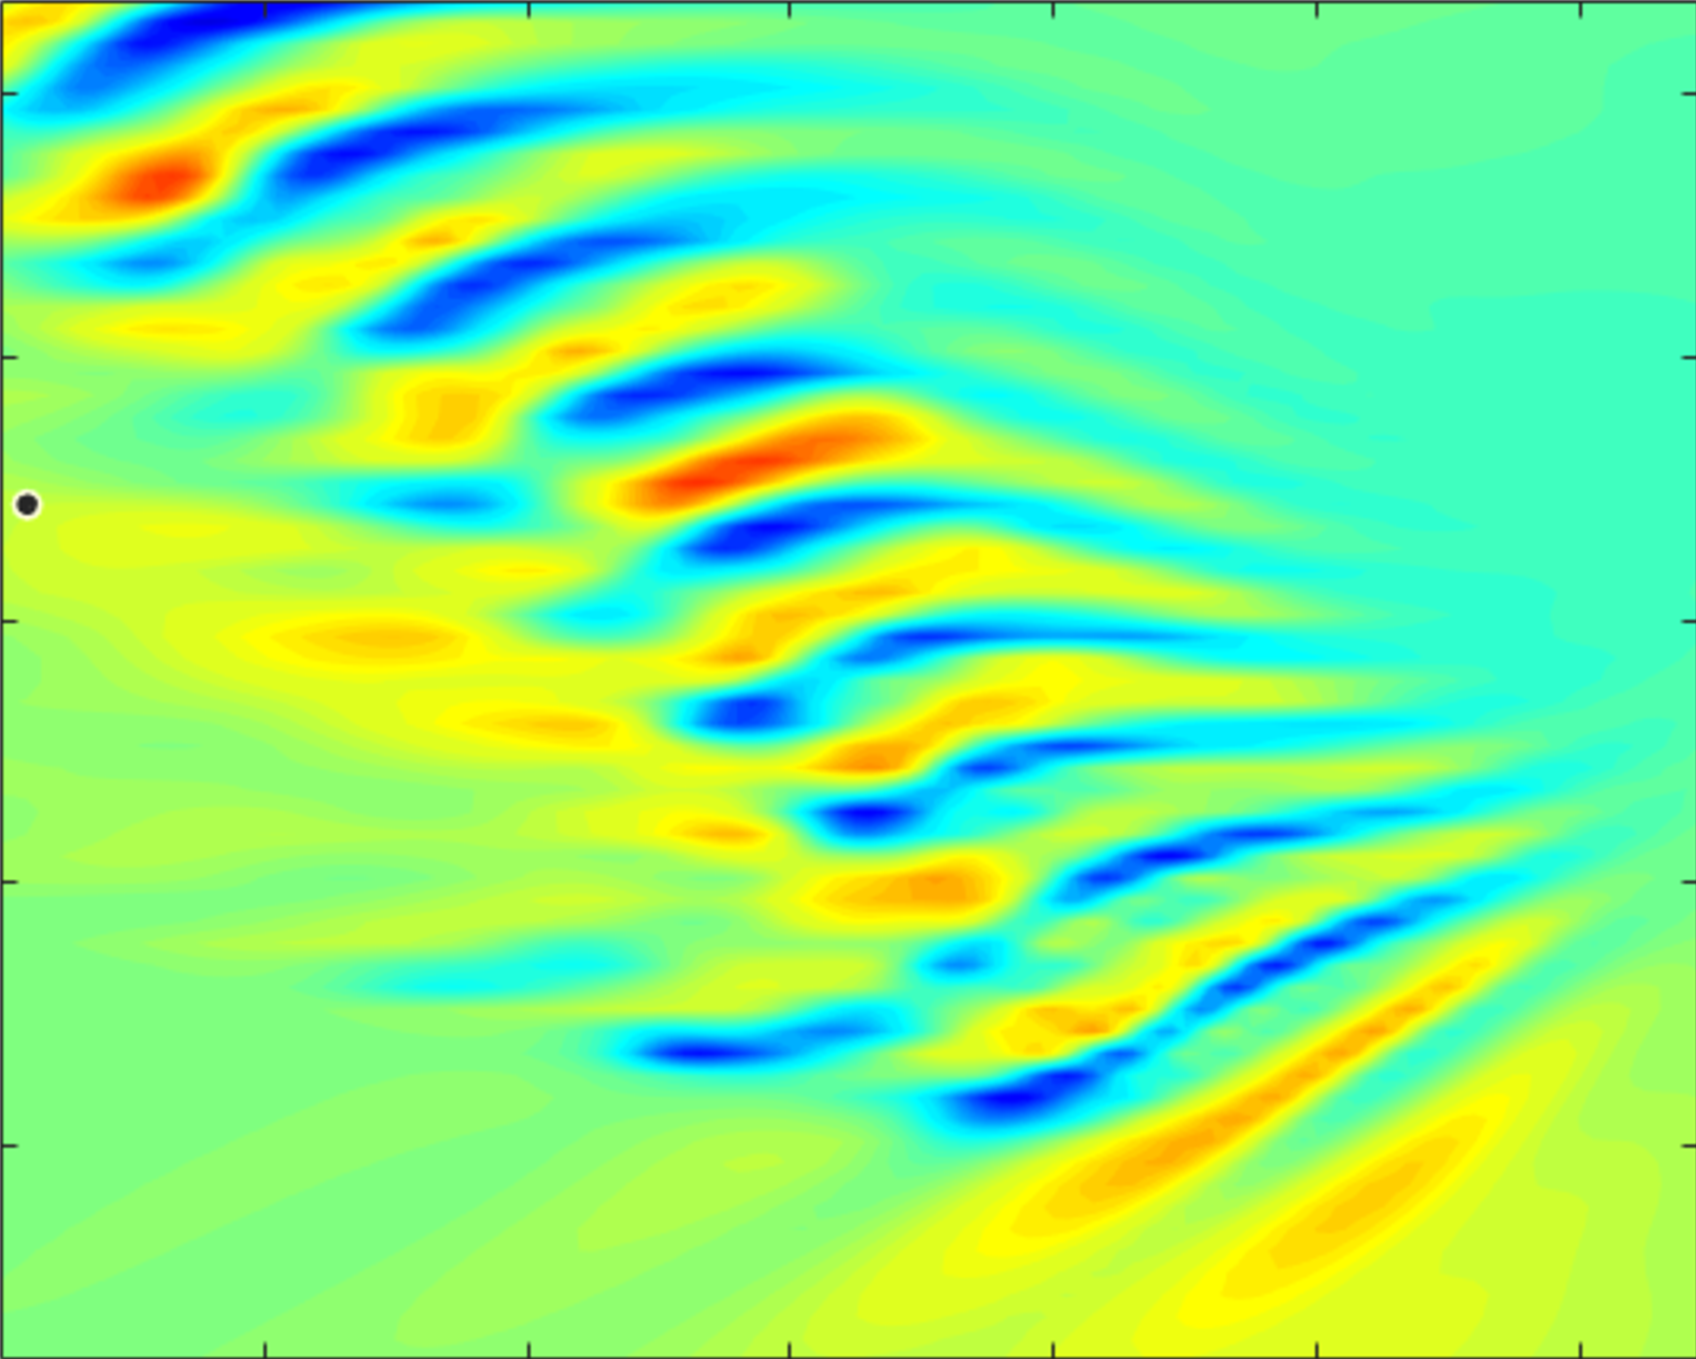
\includegraphics[width = \textwidth]{figures/prediction/actual4050.pdf}}
	\end{minipage}
	\quad
	\begin{minipage}[h]{0.22\linewidth}
	\centering
	\subfigure[t=11500]{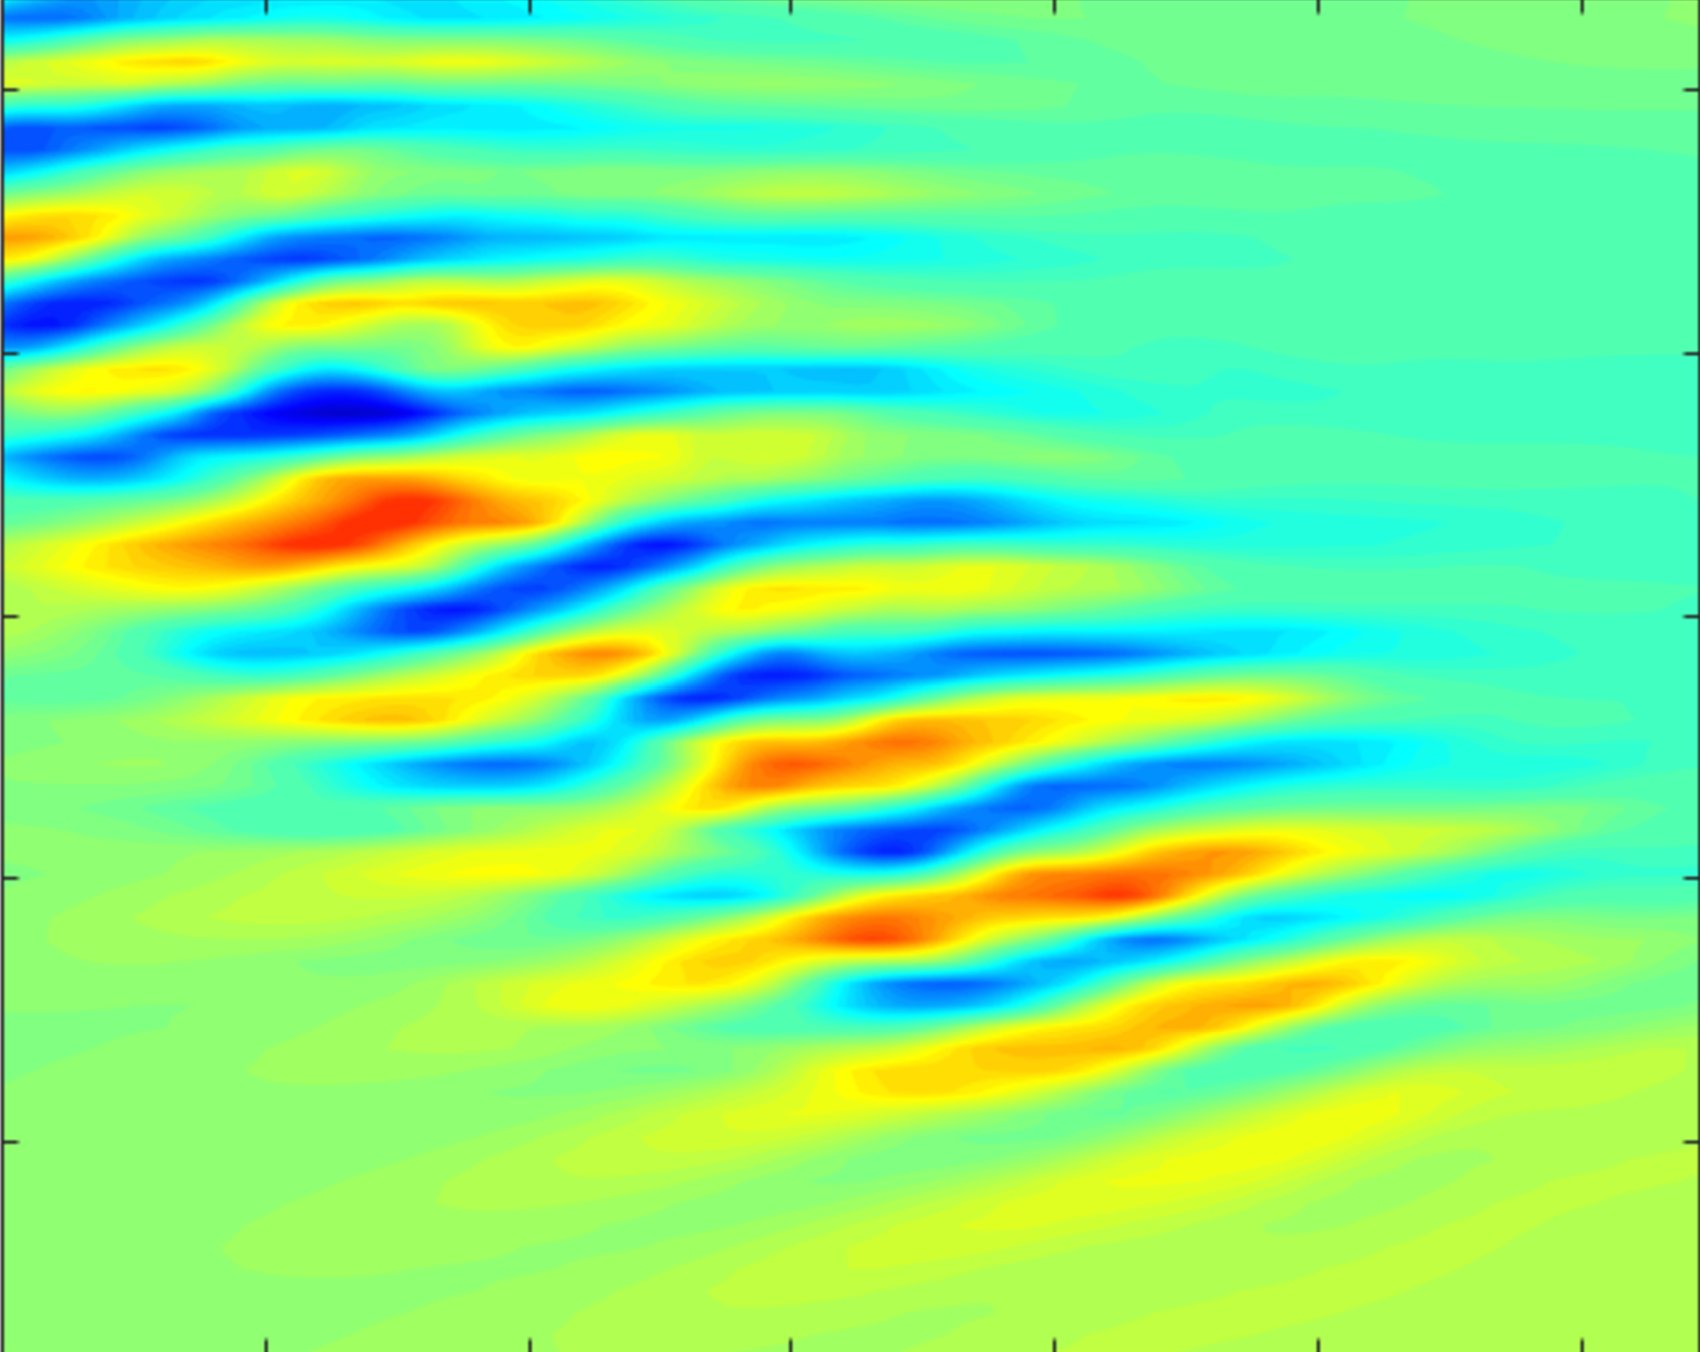
\includegraphics[width = \textwidth]{figures/prediction/actual5300.pdf}}
	\end{minipage}
	\quad
	\begin{minipage}[h]{0.22\linewidth}
	\centering
	\subfigure[ESN t=10001]{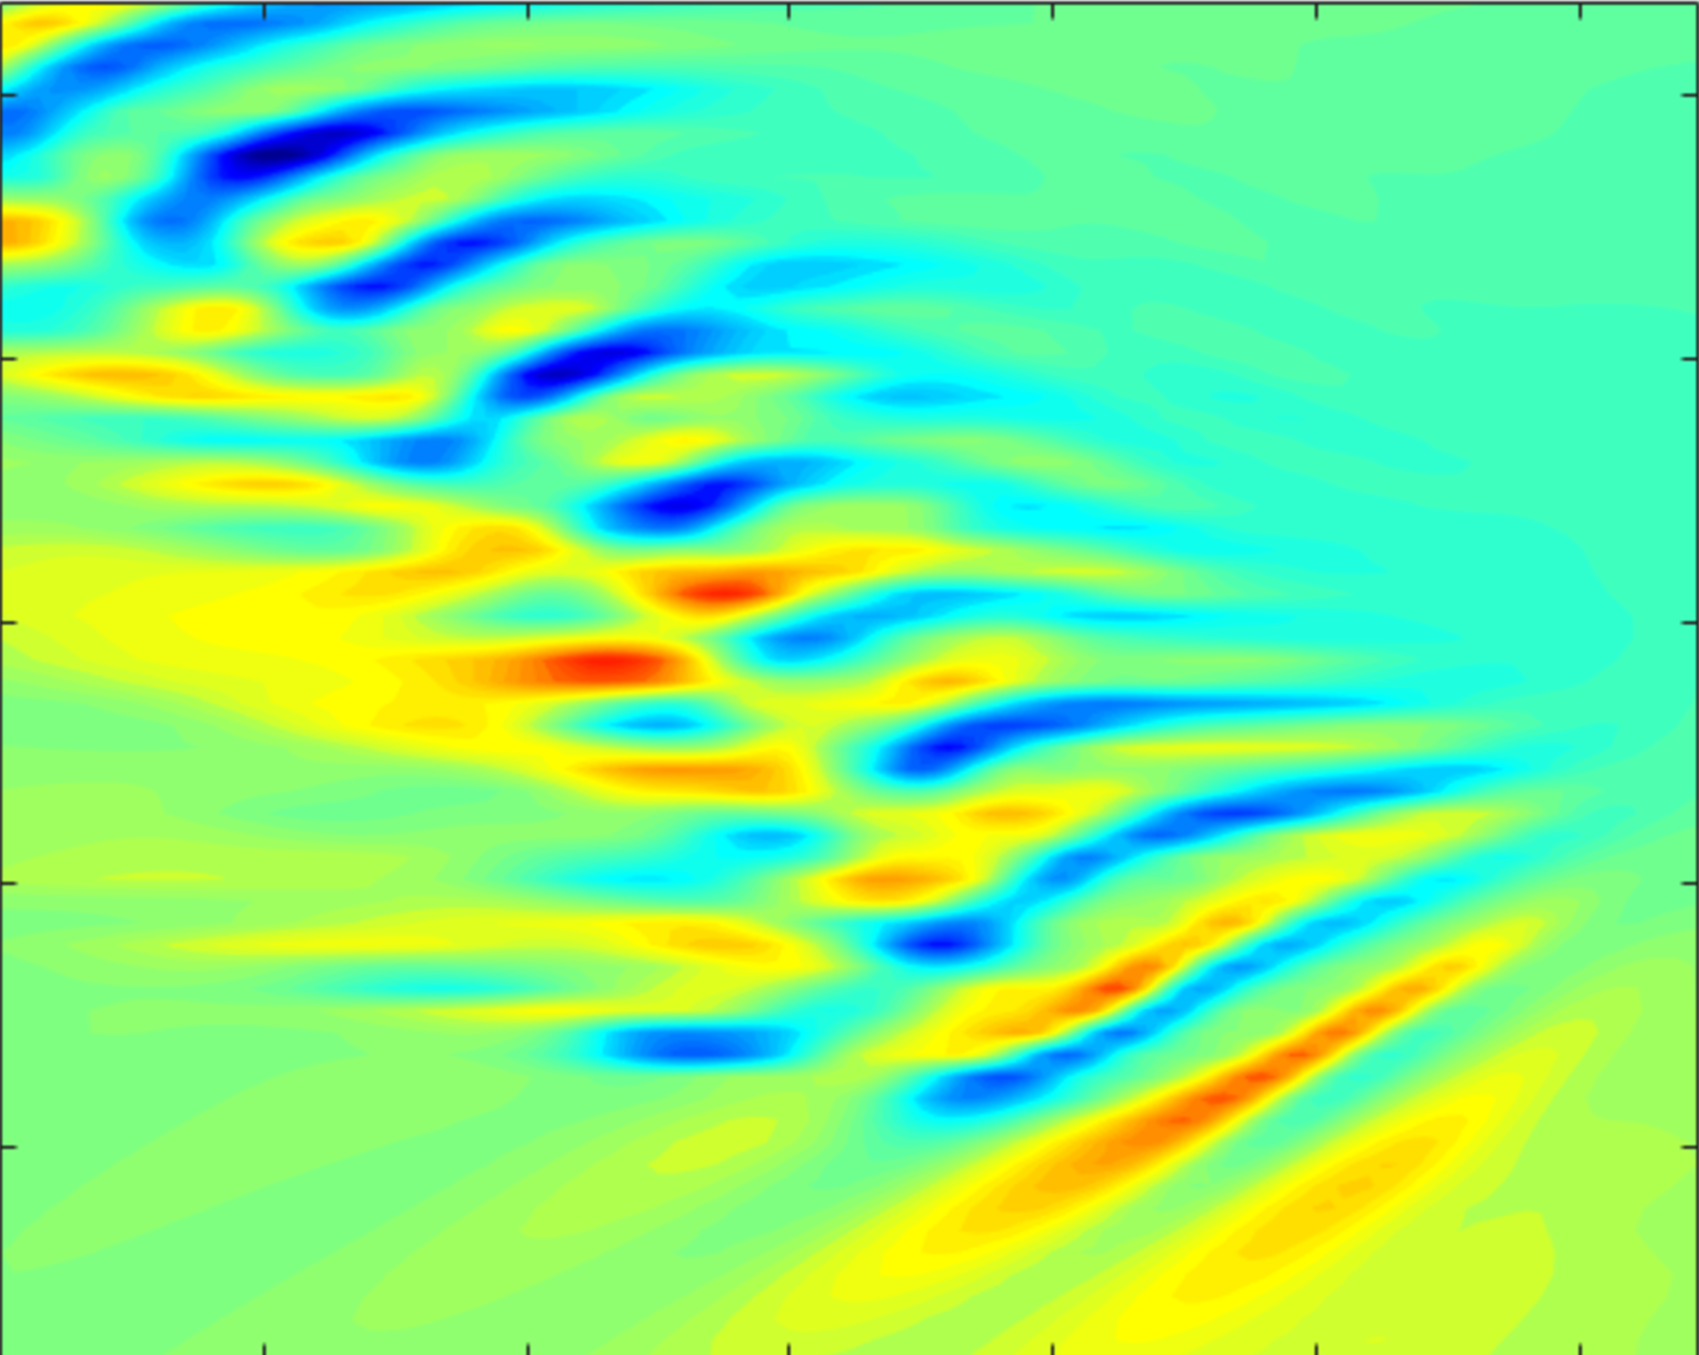
\includegraphics[width = \textwidth]{figures/prediction/ESN_pred4001.pdf}}
	\end{minipage}
	\quad
	\begin{minipage}[h]{0.22\linewidth}
	\centering
	\subfigure[t=10050]{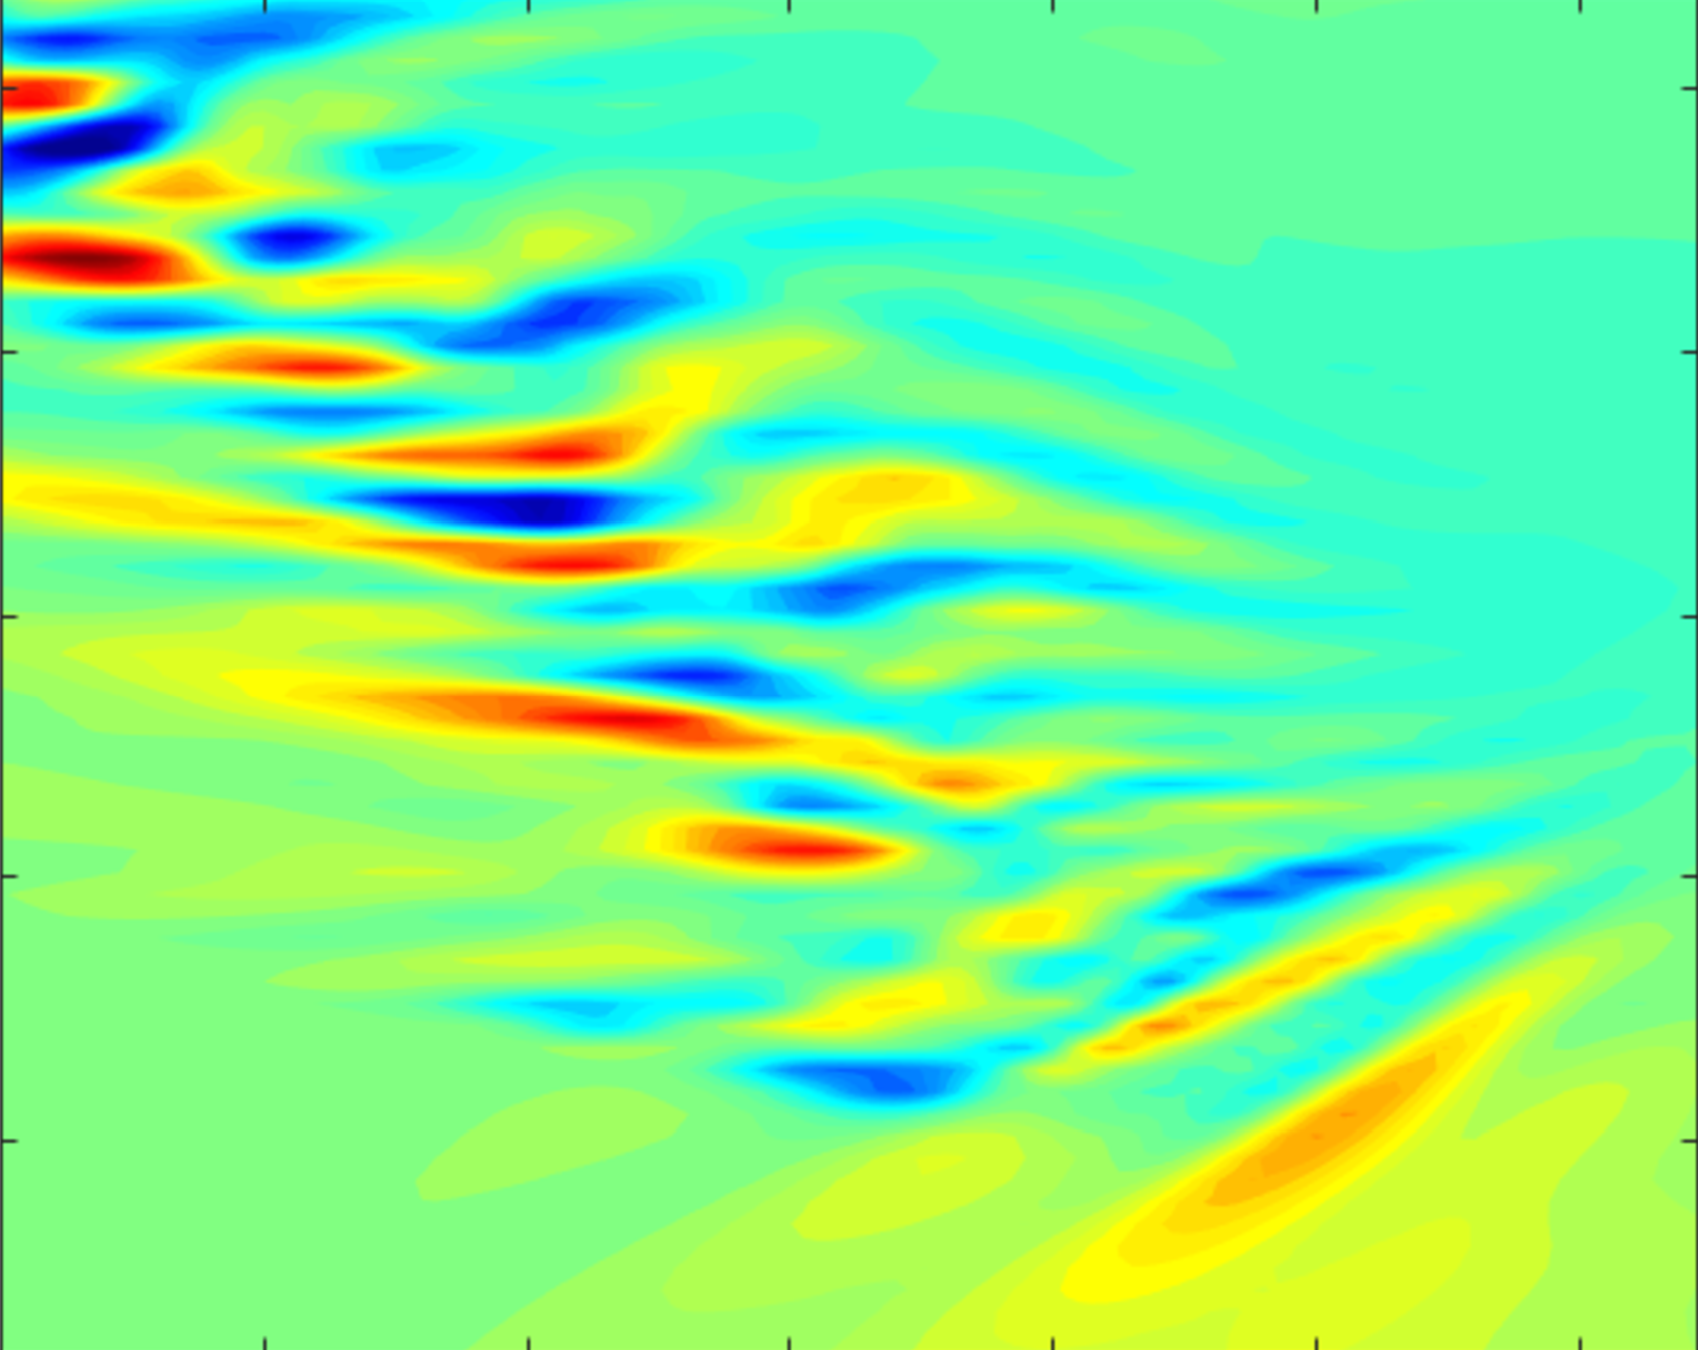
\includegraphics[width = \textwidth]{figures/prediction/ESN_pred4050.pdf}}
%	\subfigure[Re=750 t=780.5]{\includegraphics[width = 1\textwidth]{figures/side_wall/bandwall/band750-106-angle.eps}}
	\end{minipage}
	\quad
	\begin{minipage}[h]{0.22\linewidth}
	\centering
	\subfigure[t=10250]{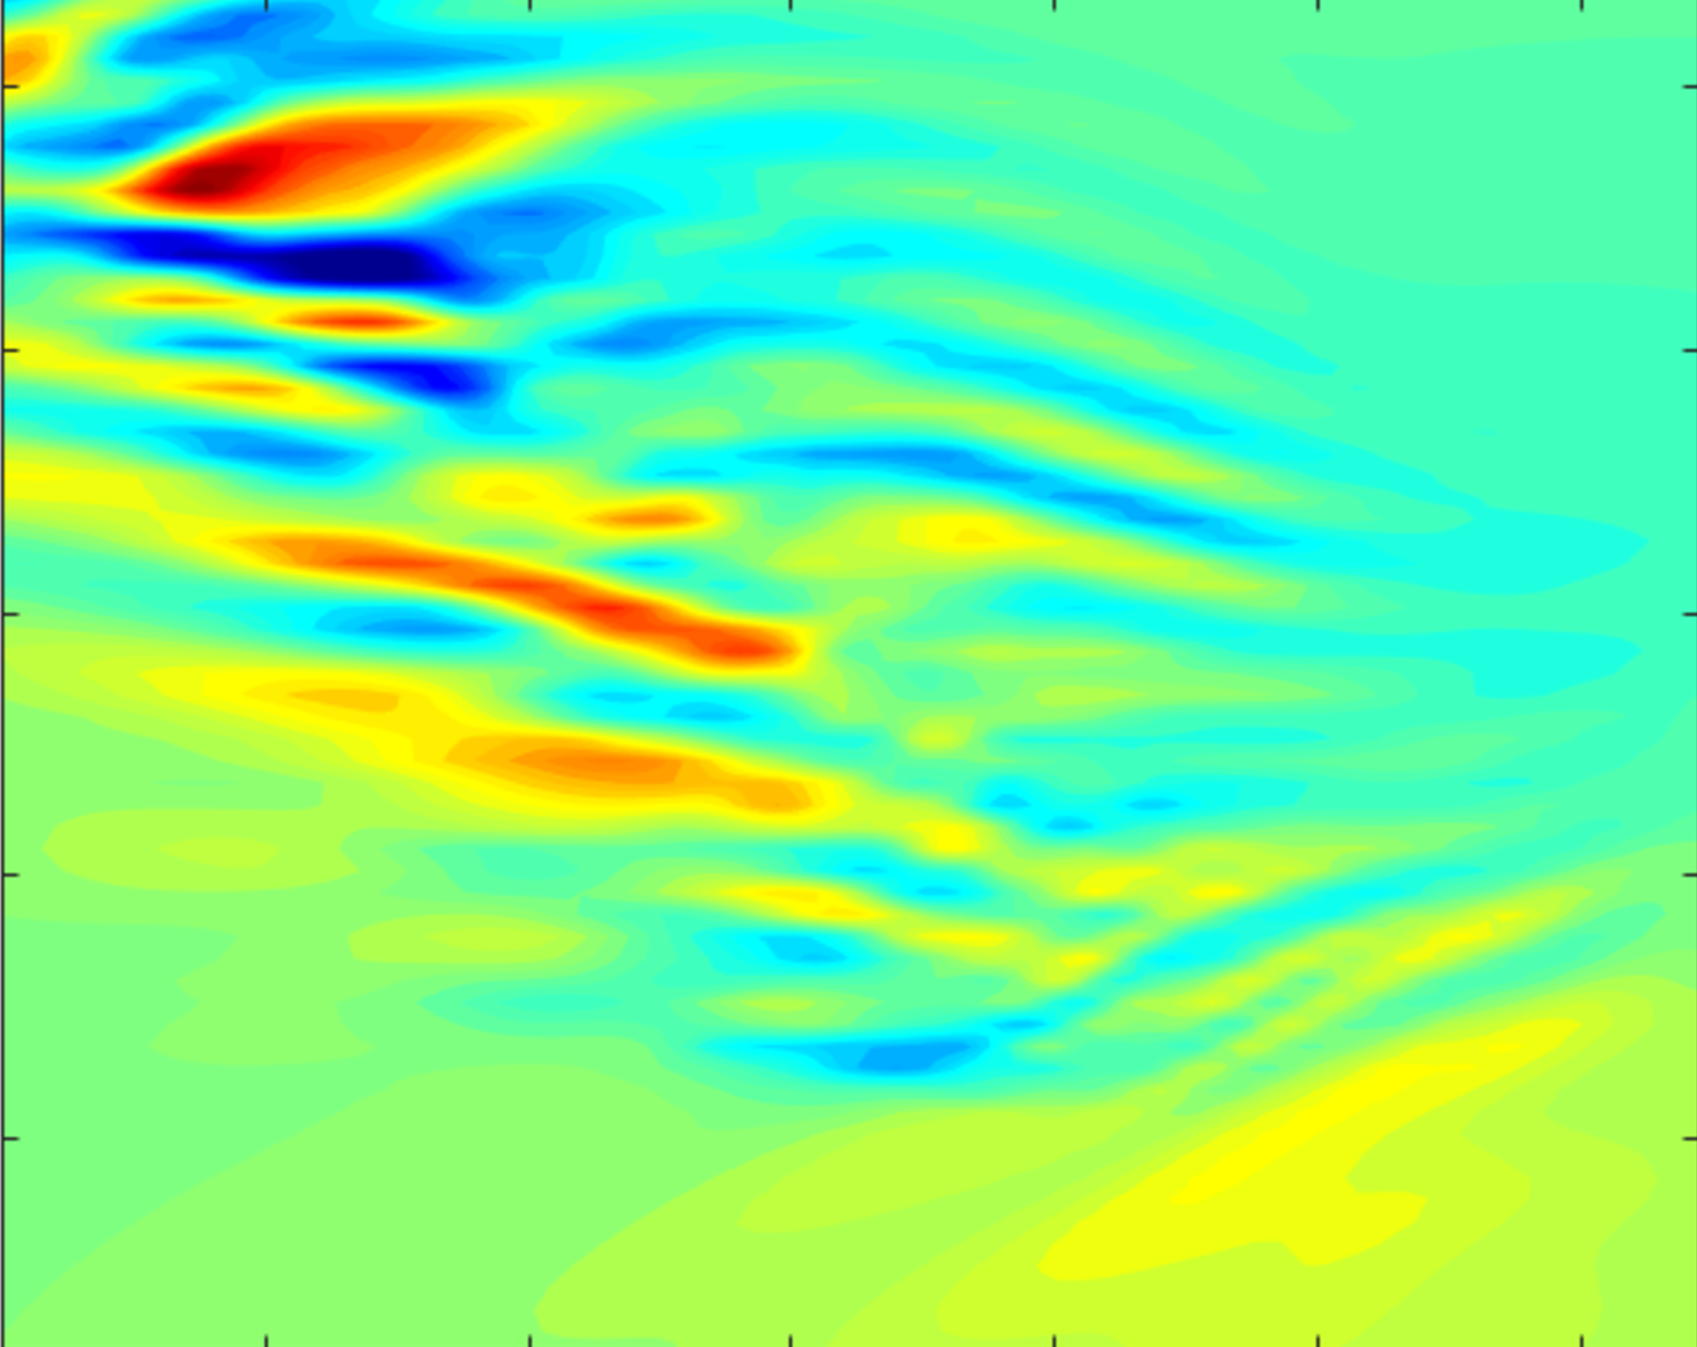
\includegraphics[width = \textwidth]{figures/prediction/ESN_pred4250.pdf}}
%	\subfigure[Re=750 t=780.5]{\includegraphics[width = 1\textwidth]{figures/side_wall/bandwall/band750-106-angle.eps}}
	\end{minipage}
	\quad
	\begin{minipage}[h]{0.22\linewidth}
	\centering
	\subfigure[t=11500]{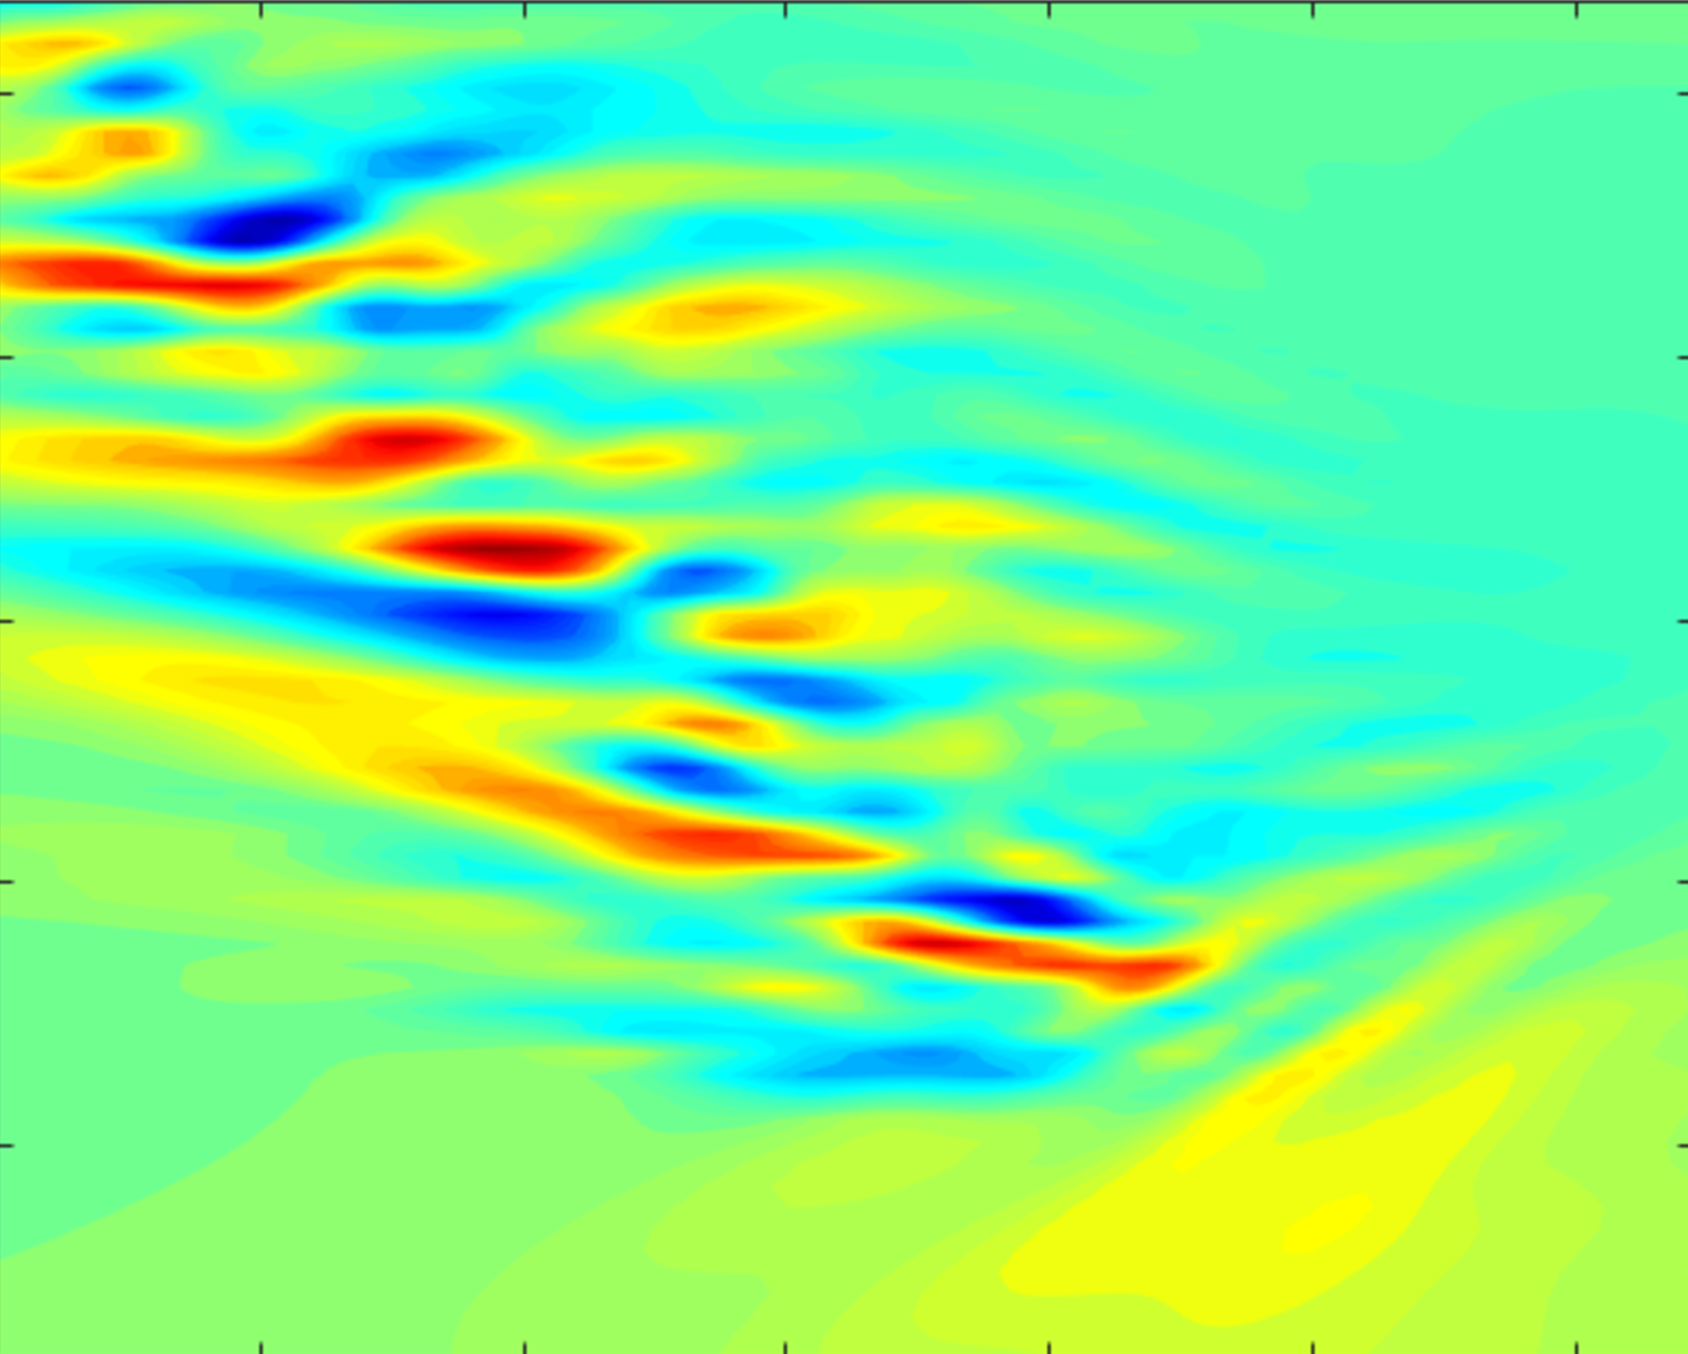
\includegraphics[width = \textwidth]{figures/prediction/ESN_pred4500.pdf}}
%	\subfigure[Re=750 t=780.5]{\includegraphics[width = 1\textwidth]{figures/side_wall/bandwall/band750-106-angle.eps}}
	\end{minipage}
	\quad
	\caption{ESN预测的流场衰减过程与实际衰减过程对比。其中a-d是实际衰减流场,e-h是ESN预测的衰减流场。可以看到ESN预测的流场虽然表现出衰减,但是与实际衰减过程相比,关键的条纹角度变化并没有预测出来。}
\label{fig:esn_decay}
\end{figure}

\subsubsection{LSTM 网络}
由于ESN方面相似研究较少,可供继续参考研究的文献不多。考虑到一般认为复杂的网络结构能提高预测准确度,本文转而尝试另外一种结构更为复杂、相关研究和落地应用更多的网络LSTM(long short term memory)。LSTM网络是RNN网络中的一种,它通过引入遗忘门机制(gating)可以长距离的记住过去的信息\cite{LSTM},提高了预测的准确度。在许多实际的时序预测任务上LSTM有相当亮眼的表现,这也是本文选择LSTM的原因。

LSTM的结构如图\ref{fig:lstm}(a)。已有的研究比较了1,2,3层LSTM在特定时间序列预测任务上的表现,得出的结论是2层的LSTM比1层有明显提升,同时3层的LSTM比2层网络没有明显提升,且在多个不同输入维度下表现差于两层LSTM,因此本文选择两层LSTM\cite{Karpathy2015VisualizingAU}。\cite{Anton2023}的作者着重强调了他们在原先的ESN结构上添加了随机因子$\bm Z$使得他们的网络有很好的泛化性,也是他们预测表现良好的关键。为了对应该随机因子,本文选择在两层LSTM层之间引入一个随机Dropout层对应随机因子。Dropout层在训练时会随机性的关闭部分神经元,\cite{dropout}提出这种随机关闭行为可以提升模型的泛化性。综上所述,本文设置了如图\ref{fig:lstm}(b)的网络结构。
\begin{figure}[H]
	\subfigbottomskip = 2pt
	%\subfigcapskip=-5pt
	\begin{minipage}[h]{1\linewidth}
	\centering
	\subfigure[]{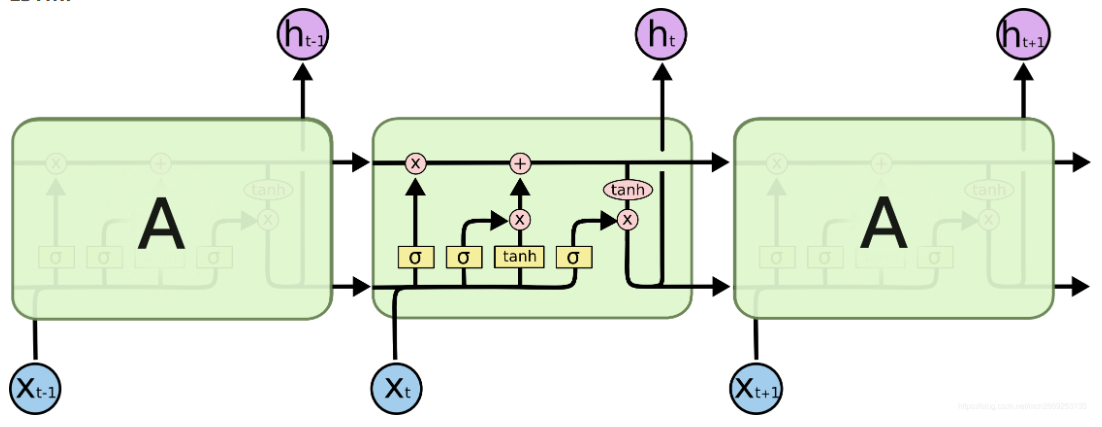
\includegraphics[width = \textwidth]{figures/prediction/LSTM_structure.png}}
	\end{minipage}
	\quad
	\subfigbottomskip = 2pt
	\subfigcapskip=-5pt
	\begin{minipage}[h]{\linewidth}
	\centering
	\subfigure[]{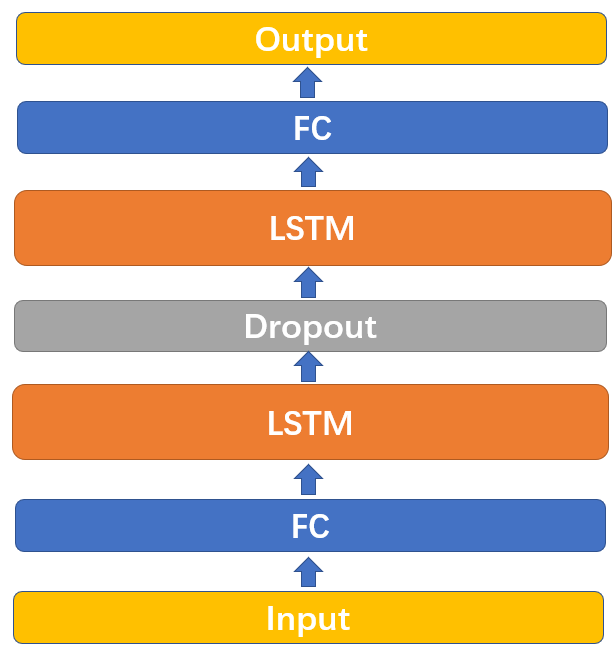
\includegraphics[width = 0.6\textwidth]{figures/prediction/LSTM_mvstructure.png}}
	\end{minipage}
	\quad
	\caption{(a)LSTM结构示意图,采取了更多的非线性函数构造门结构记忆历史数据。(b)本文中采取的双层LSTM网络结构示意图。两层中间插入了随机关闭层dropout以增加泛化性。}
\label{fig:lstm}
\end{figure}

在文献\cite{lstmmodes}中,作者通过LSTM模拟预测了圆柱绕流的流场变化。其中采用了20个POD主模态重构(TKE贡献度90\%),隐藏层大小为200。基于该组超参数组合综合考虑时间成本和计算成本,本文中LSTM设置输入的POD模数为50(TKE贡献度80\%),隐藏层大小为500。搭建好神经网络后采用相同的训练思路,输入上一个流场的模数得出下一个流场模数,这同时也是\cite{Pandey2020}中所采用的方法。图\ref{fig:lstm_purepred}是LSTM预测的后续流场变化以及与实际流场的比较。可以看出比起ESN,LSTM预测出的流场保持了湍流带的几个重要力学特征,包括强度较高的头部,头部的条纹生成机制等。且从图\ref{fig:LSTM_angle_eny}流场能量的变化对比可以看出,在刚开始的时间段内,LSTM预测的流场能量变化趋势与实际能量趋势有一定的重合度,这证明LSTM确实通过历史数据捕捉到了湍流带演化的关键力学机制。然而也能发现,在后续的继续演化中LSTM的湍流带并没有展现出衰减的趋势,且好像陷入了某个周期稳定的解上,并没能预测出衰减的现象。
\begin{figure}[H]
	\subfigbottomskip = 2pt
	%\subfigcapskip=-5pt
	\begin{minipage}[h]{0.24\linewidth}
	\centering
	\subfigure[LSTM t=10001]{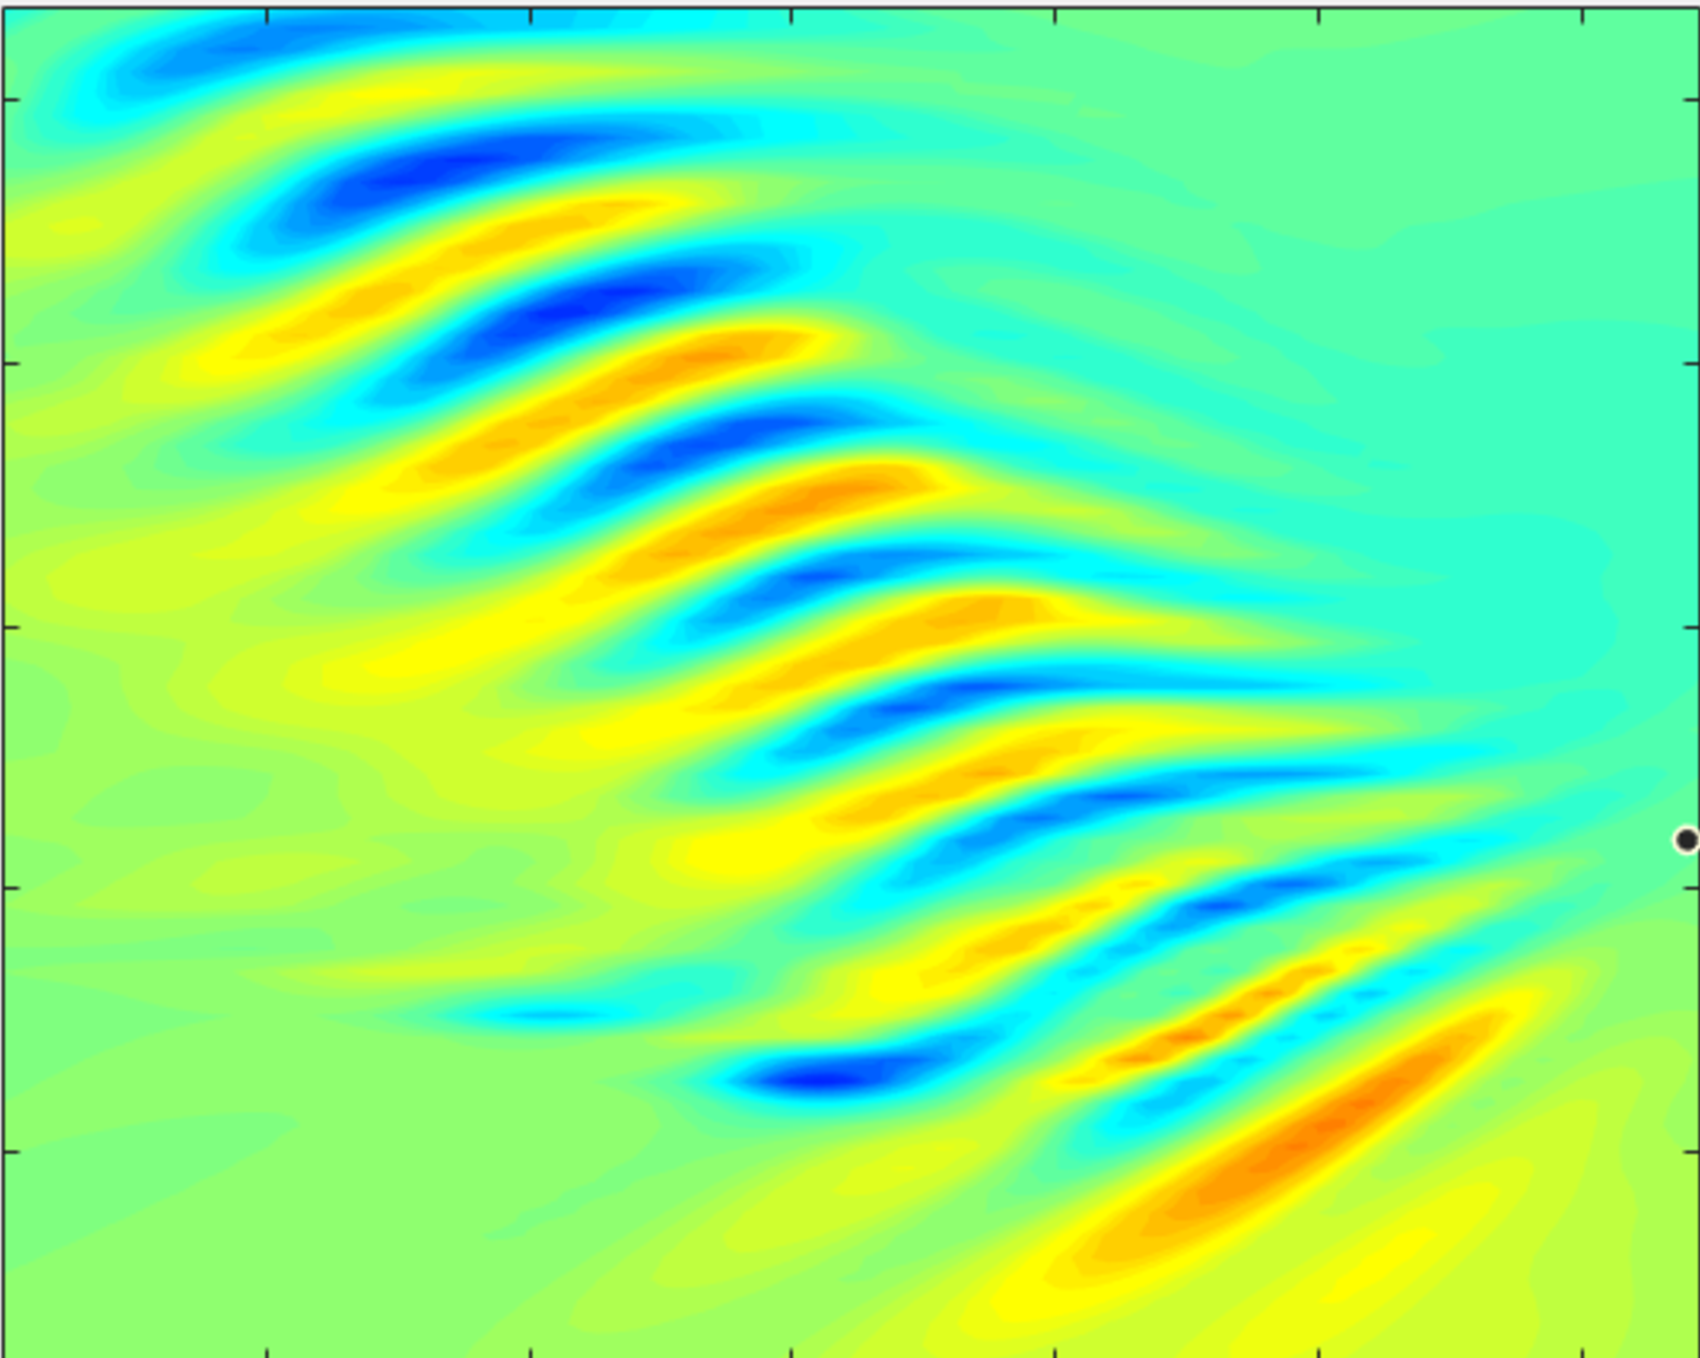
\includegraphics[width = \textwidth]{figures/prediction/lstm_pure_4001.pdf}}
	\end{minipage}
	\begin{minipage}[h]{0.24\linewidth}
	\centering
	\subfigure[t=10100]{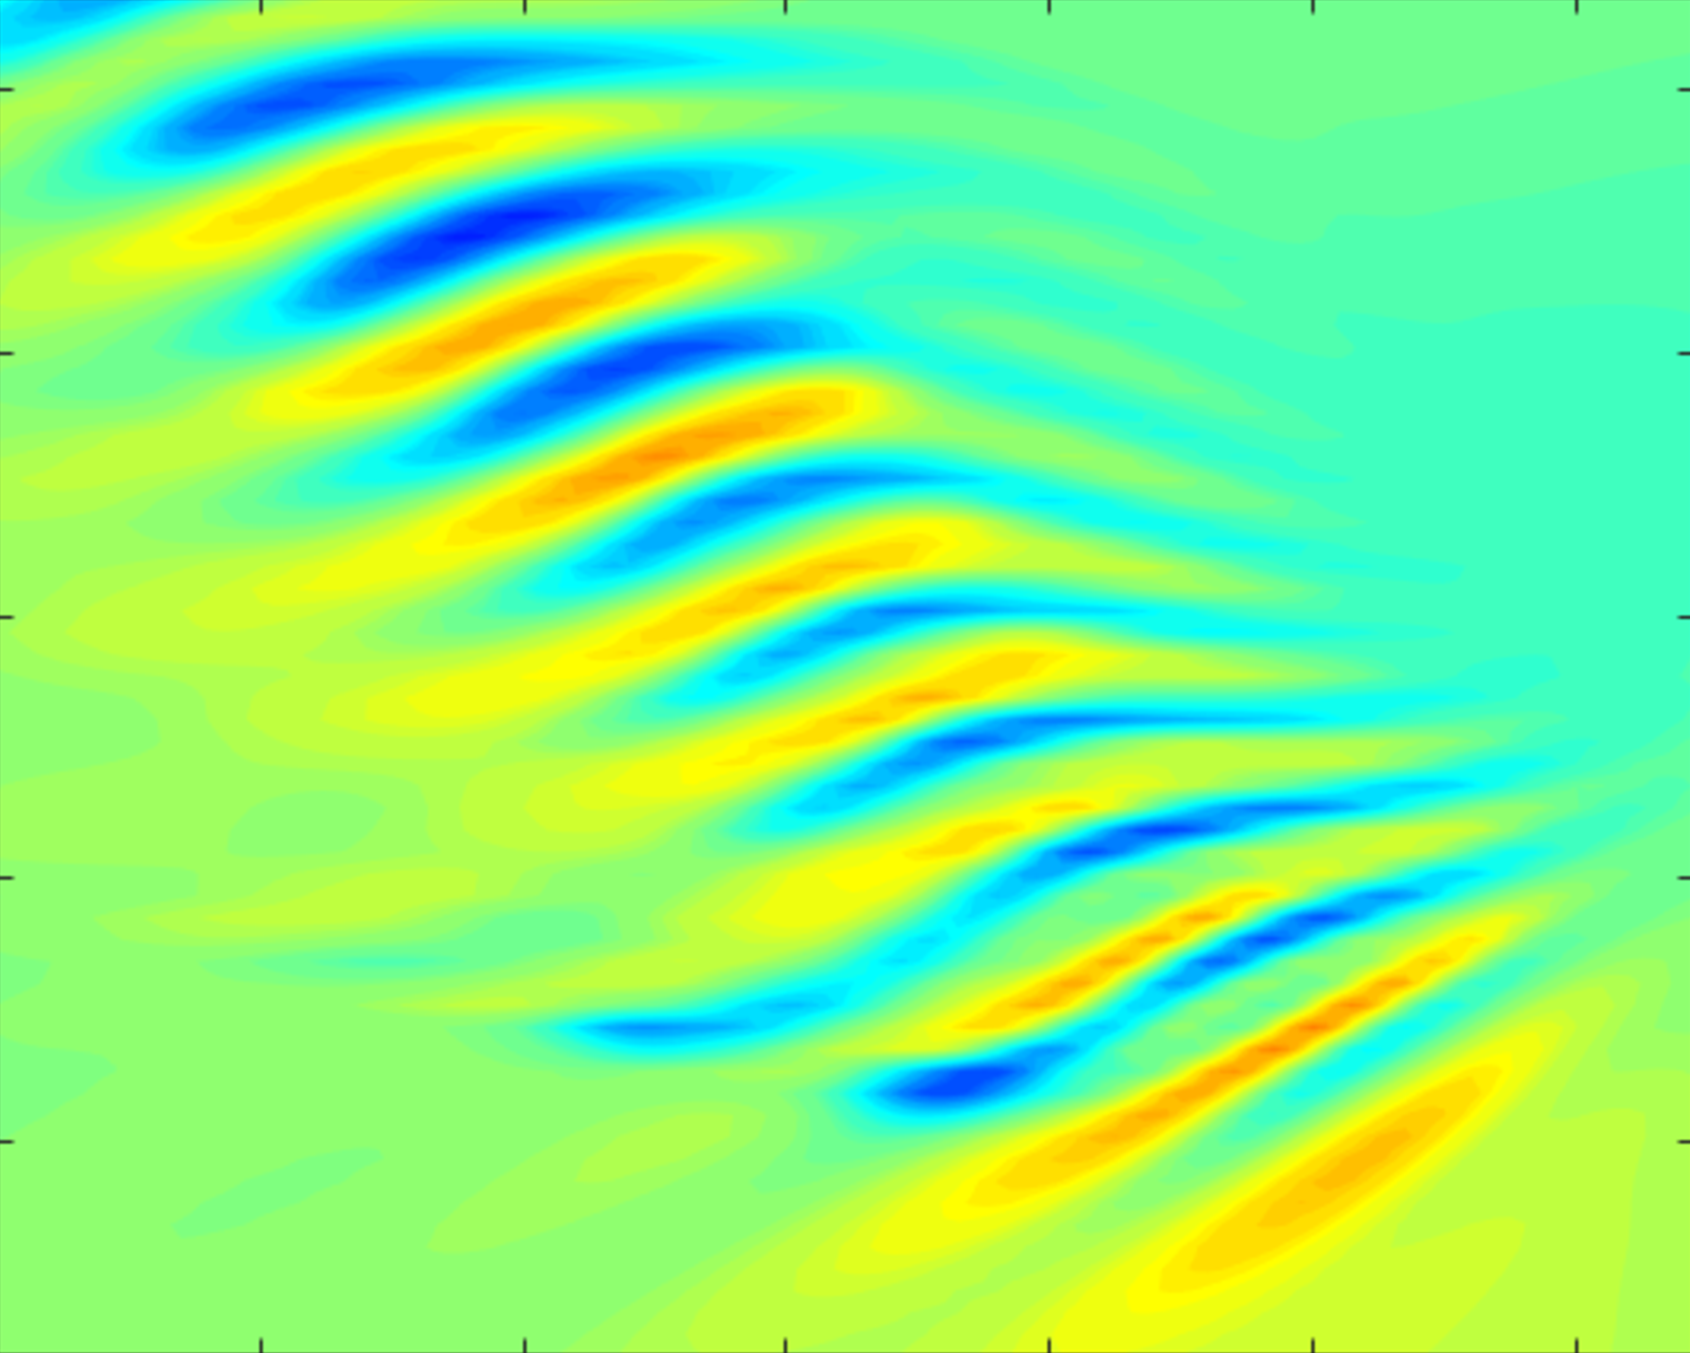
\includegraphics[width = \textwidth]{figures/prediction/lstm_pure_4100.pdf}}
	\end{minipage}
	\begin{minipage}[h]{0.24\linewidth}
	\centering
	\subfigure[t=11000]{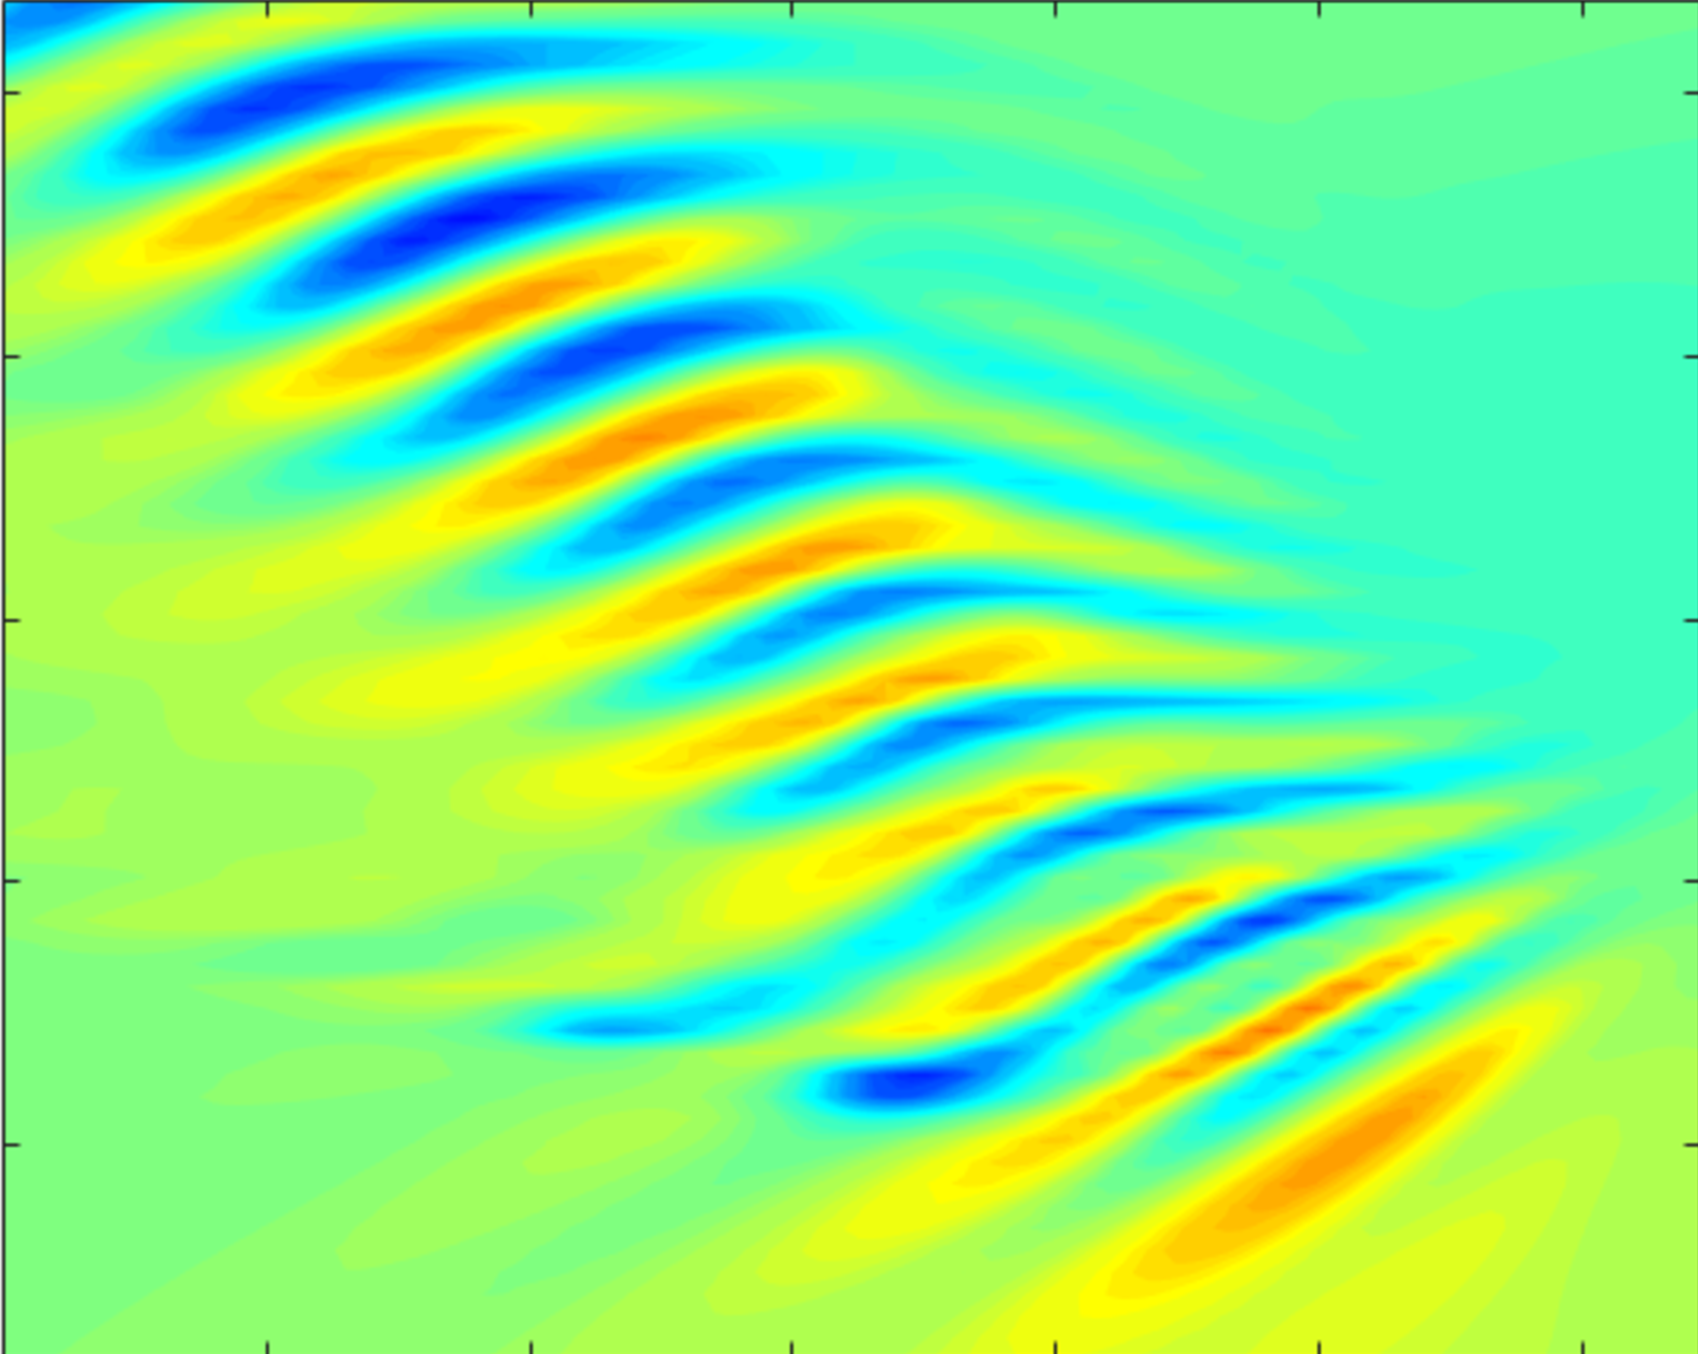
\includegraphics[width = \textwidth]{figures/prediction/lstm_pure_5000.pdf}}
	\end{minipage}
	\begin{minipage}[h]{0.24\linewidth}
	\centering
	\subfigure[t=14000]{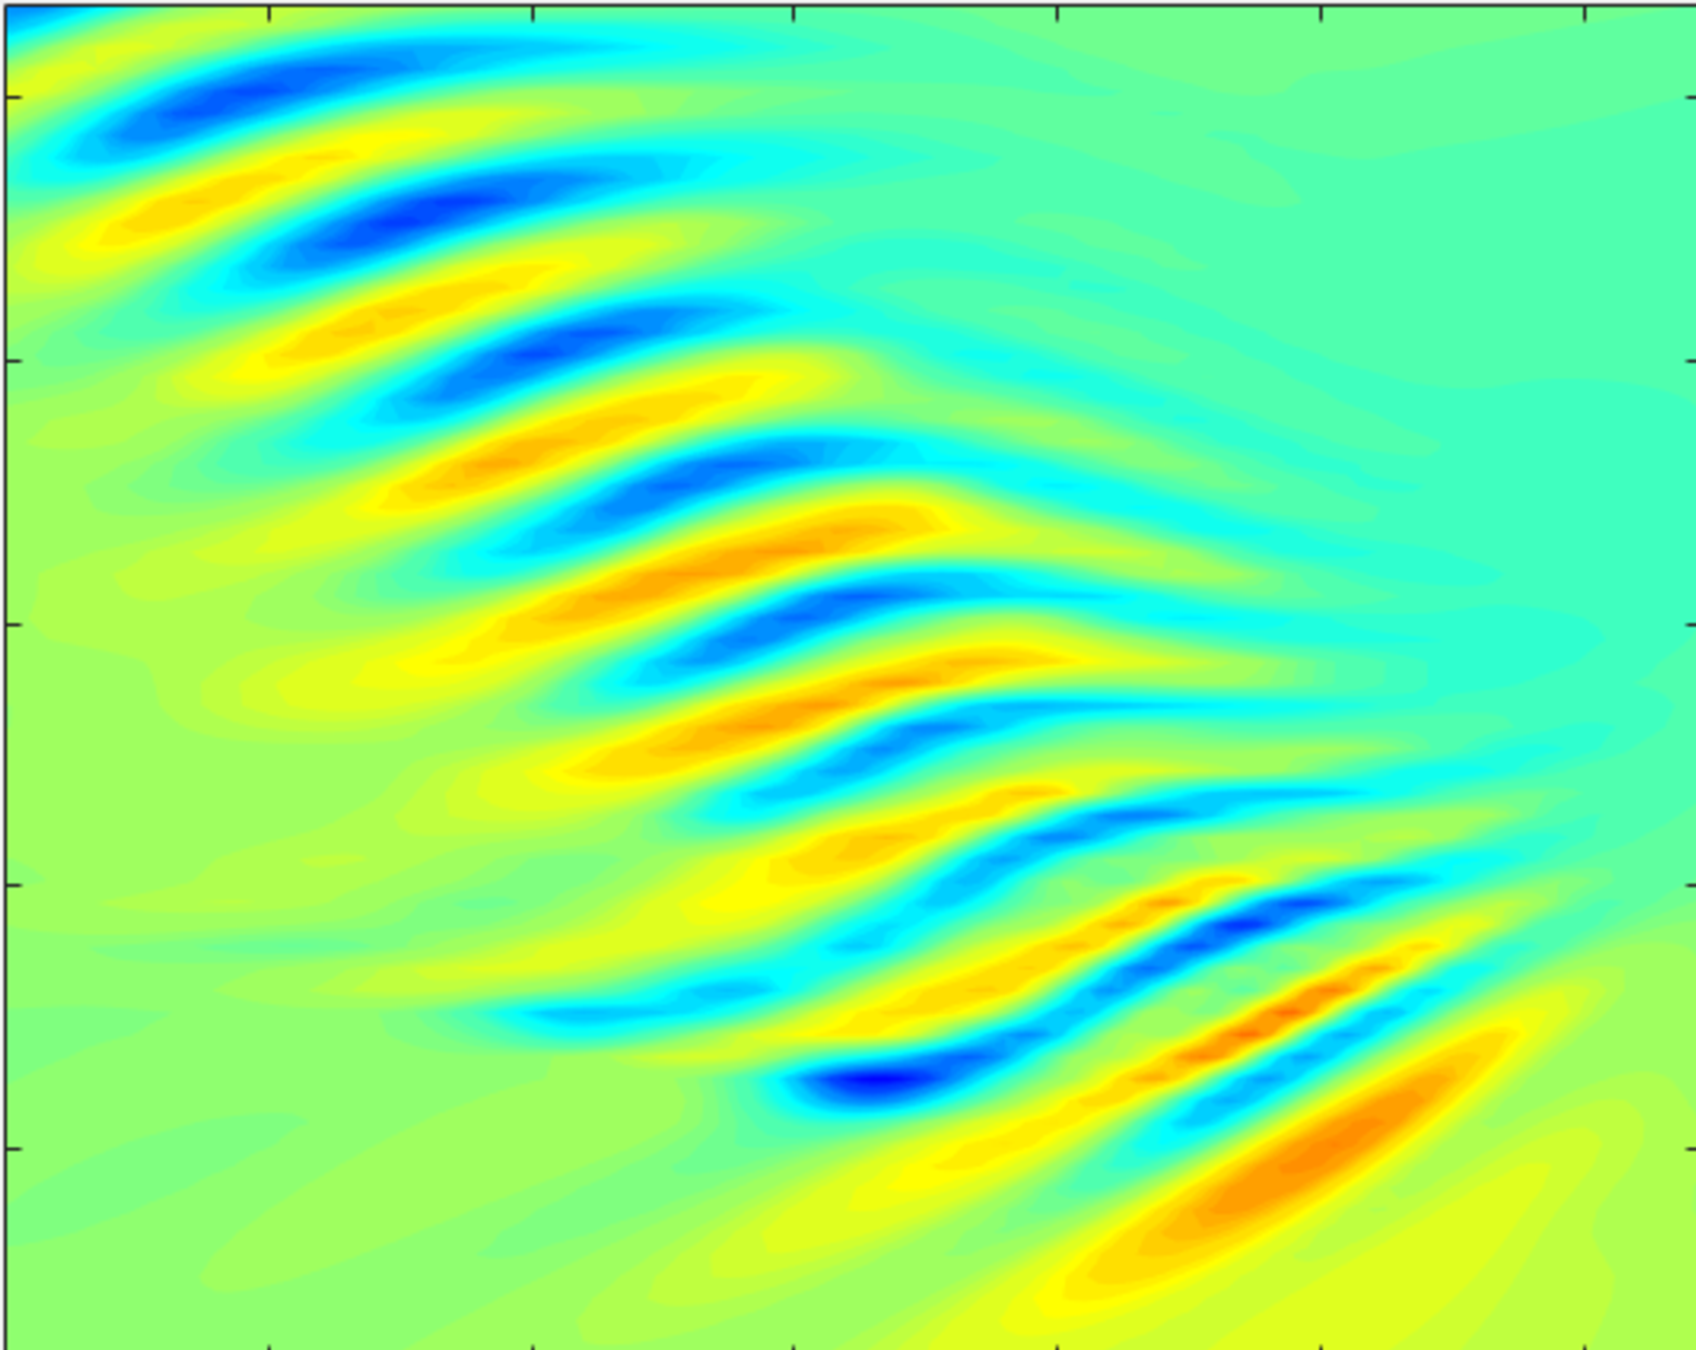
\includegraphics[width = 1\textwidth]{figures/prediction/lstm_pure_8000.pdf}}
	\end{minipage}
	
	\begin{minipage}[h]{0.24\linewidth}
	\centering
	\subfigure[actual t=10001]{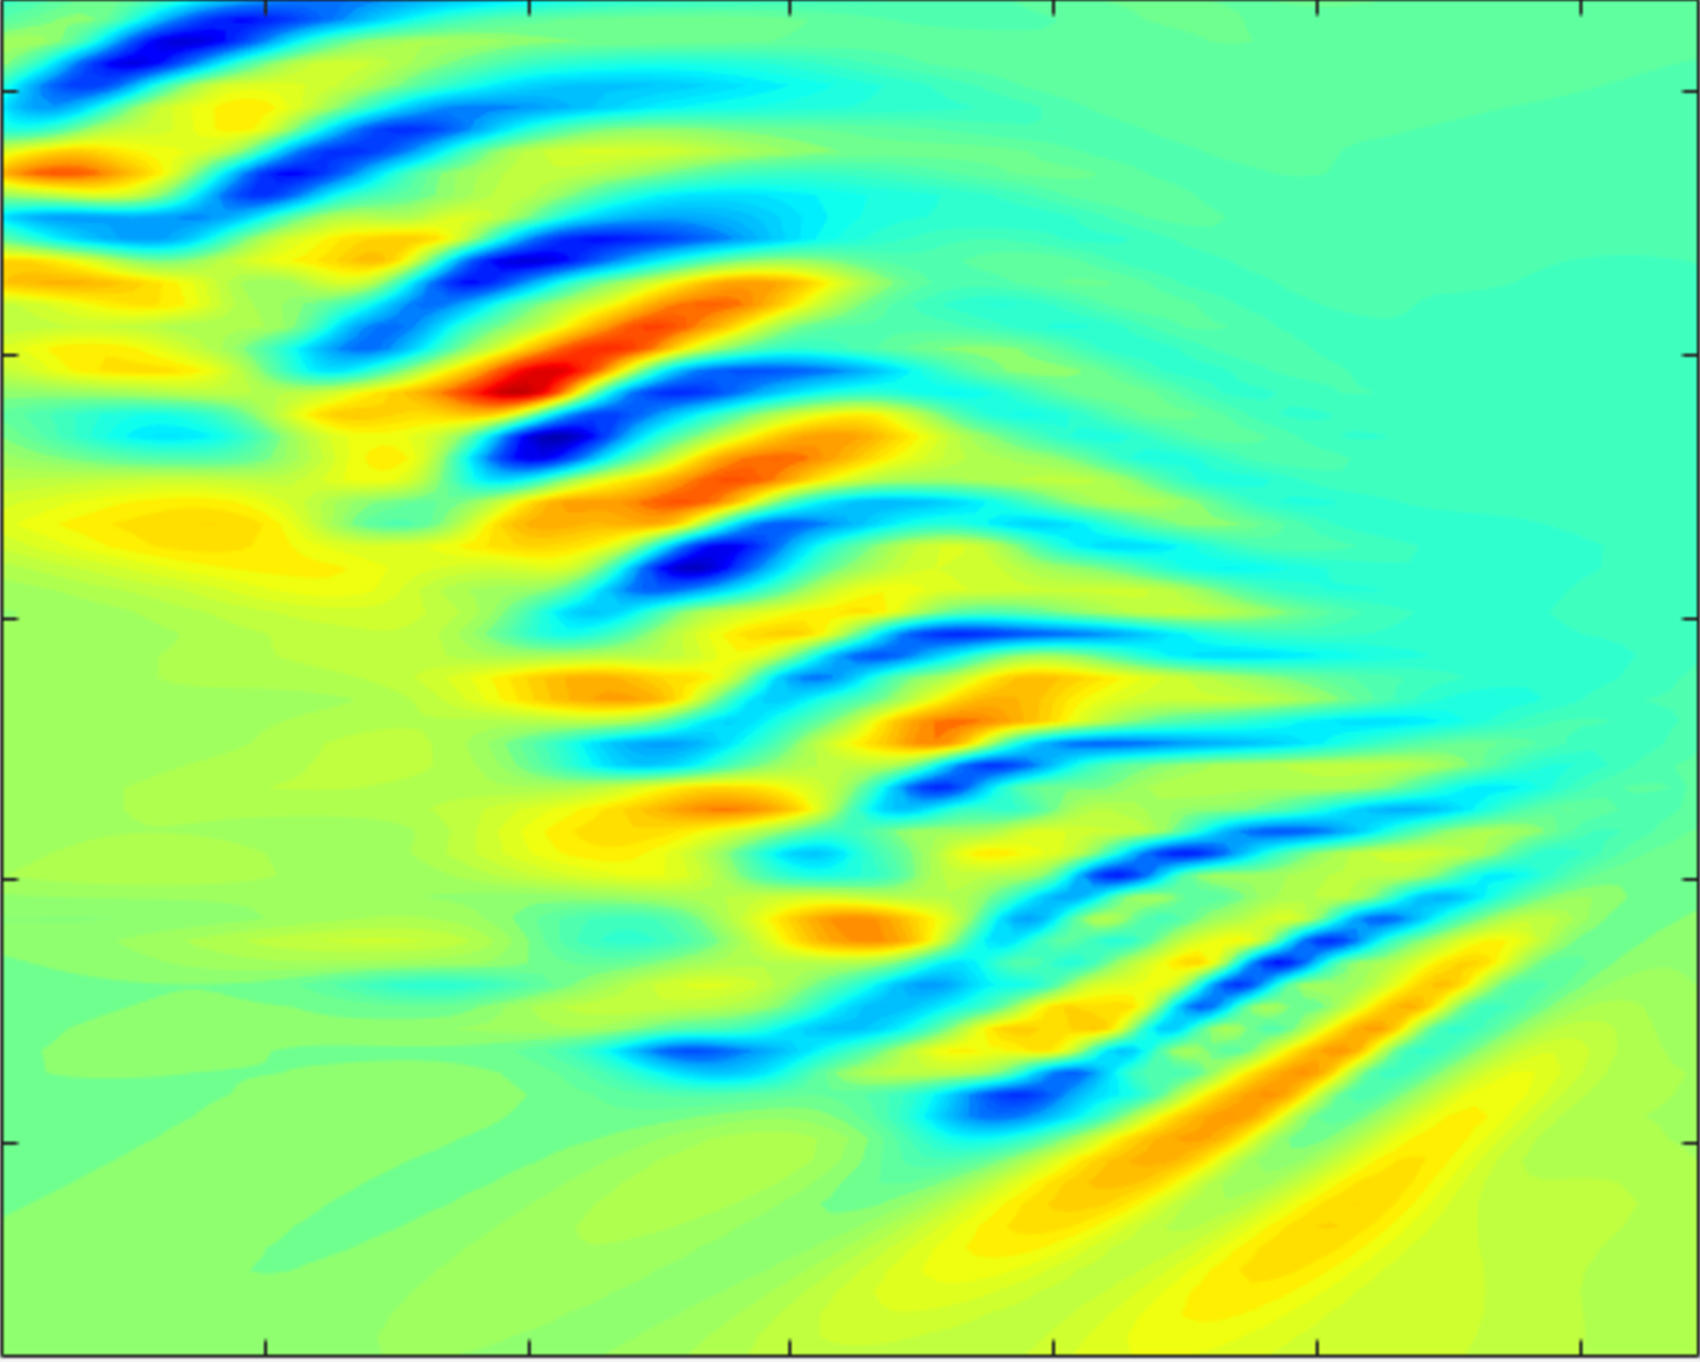
\includegraphics[width = \textwidth]{figures/prediction/actual4001.pdf}}
	\end{minipage}
	\begin{minipage}[h]{0.24\linewidth}
	\centering
	\subfigure[t=10050]{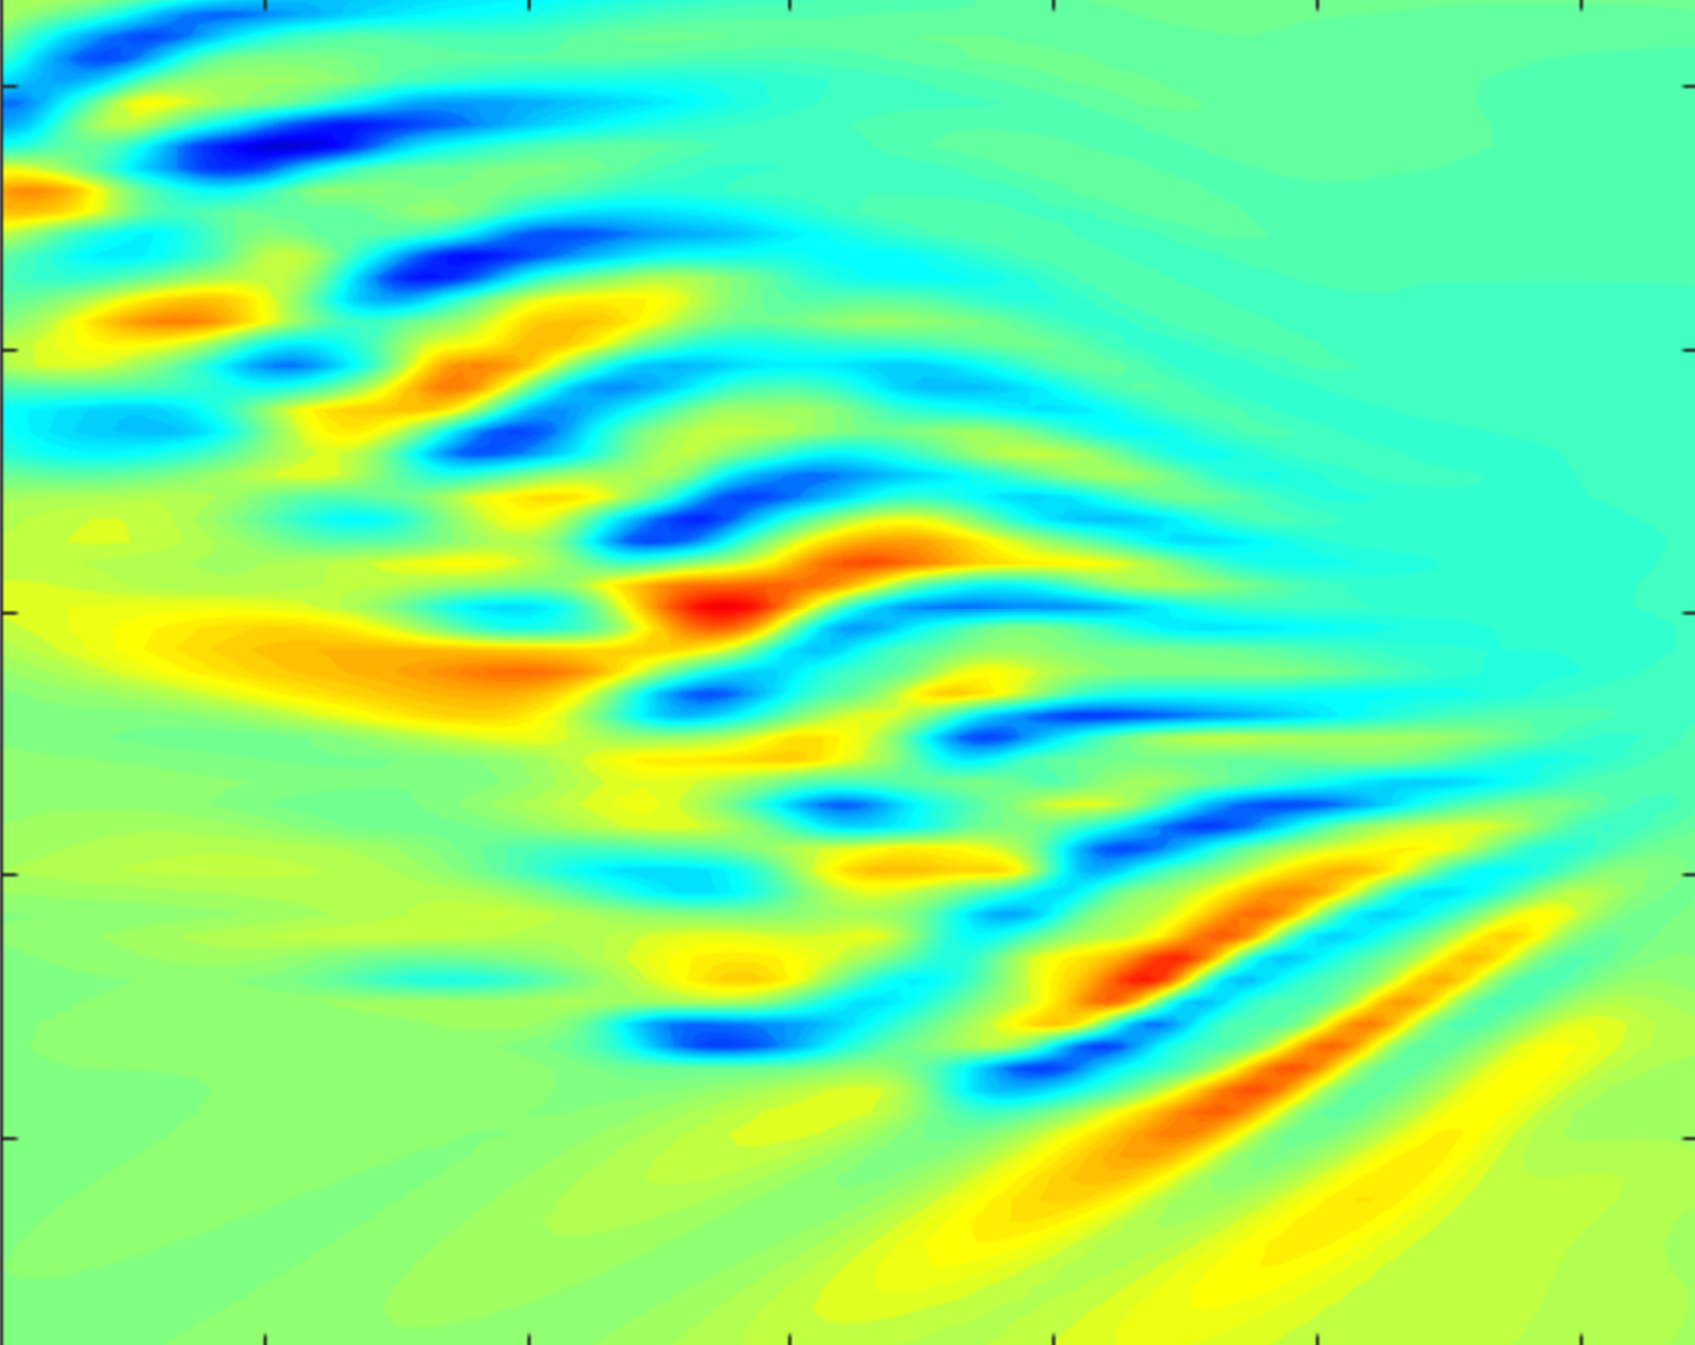
\includegraphics[width = \textwidth]{figures/prediction/actual4250.pdf}}
%	\subfigure[Re=750 t=780.5]{\includegraphics[width = 1\textwidth]{figures/side_wall/bandwall/band750-106-angle.eps}}
	\end{minipage}
	\begin{minipage}[h]{0.24\linewidth}
	\centering
	\subfigure[t=10250]{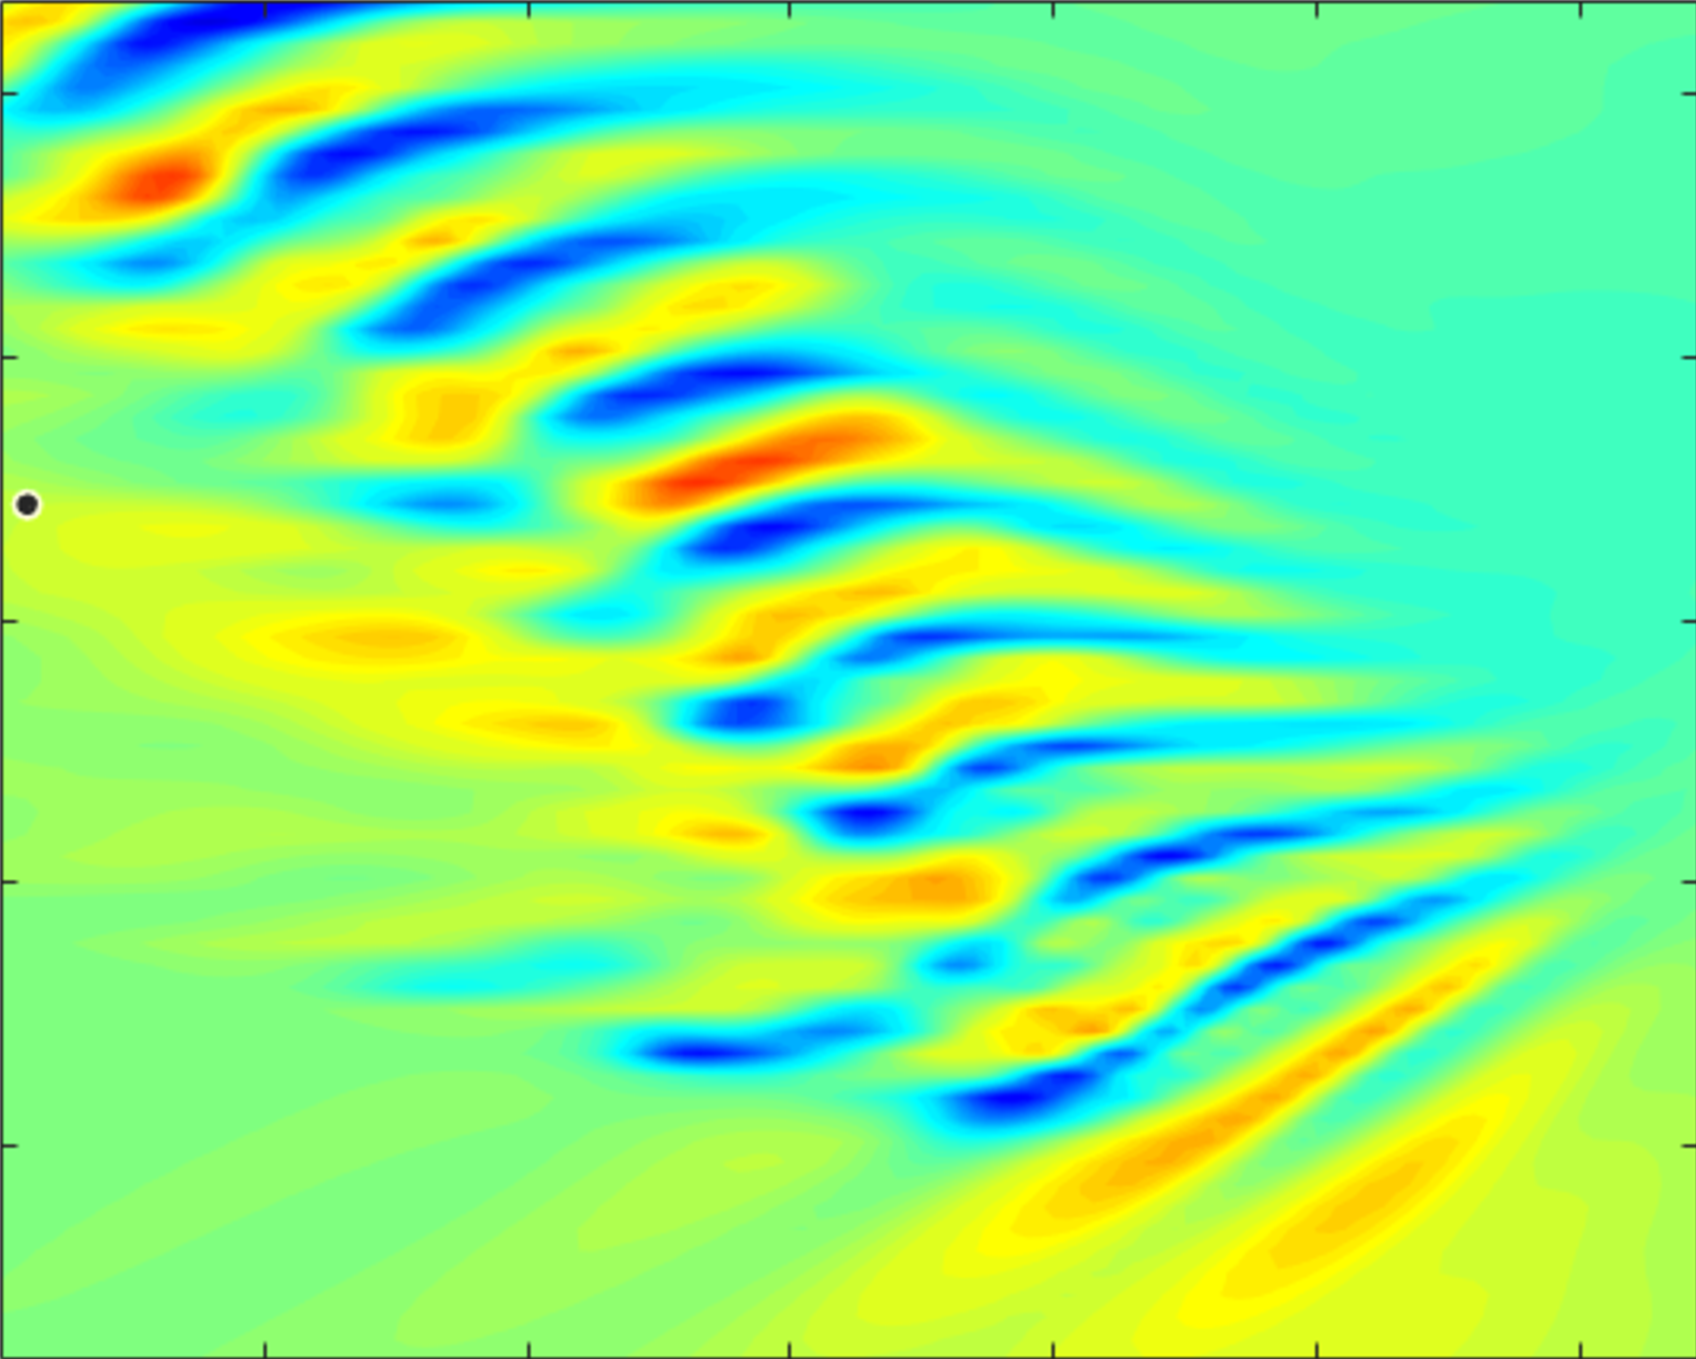
\includegraphics[width = \textwidth]{figures/prediction/actual4050.pdf}}
%	\subfigure[Re=750 t=780.5]{\includegraphics[width = 1\textwidth]{figures/side_wall/bandwall/band750-106-angle.eps}}
	\end{minipage}
	\begin{minipage}[h]{0.24\linewidth}
	\centering
	\subfigure[t=11500]{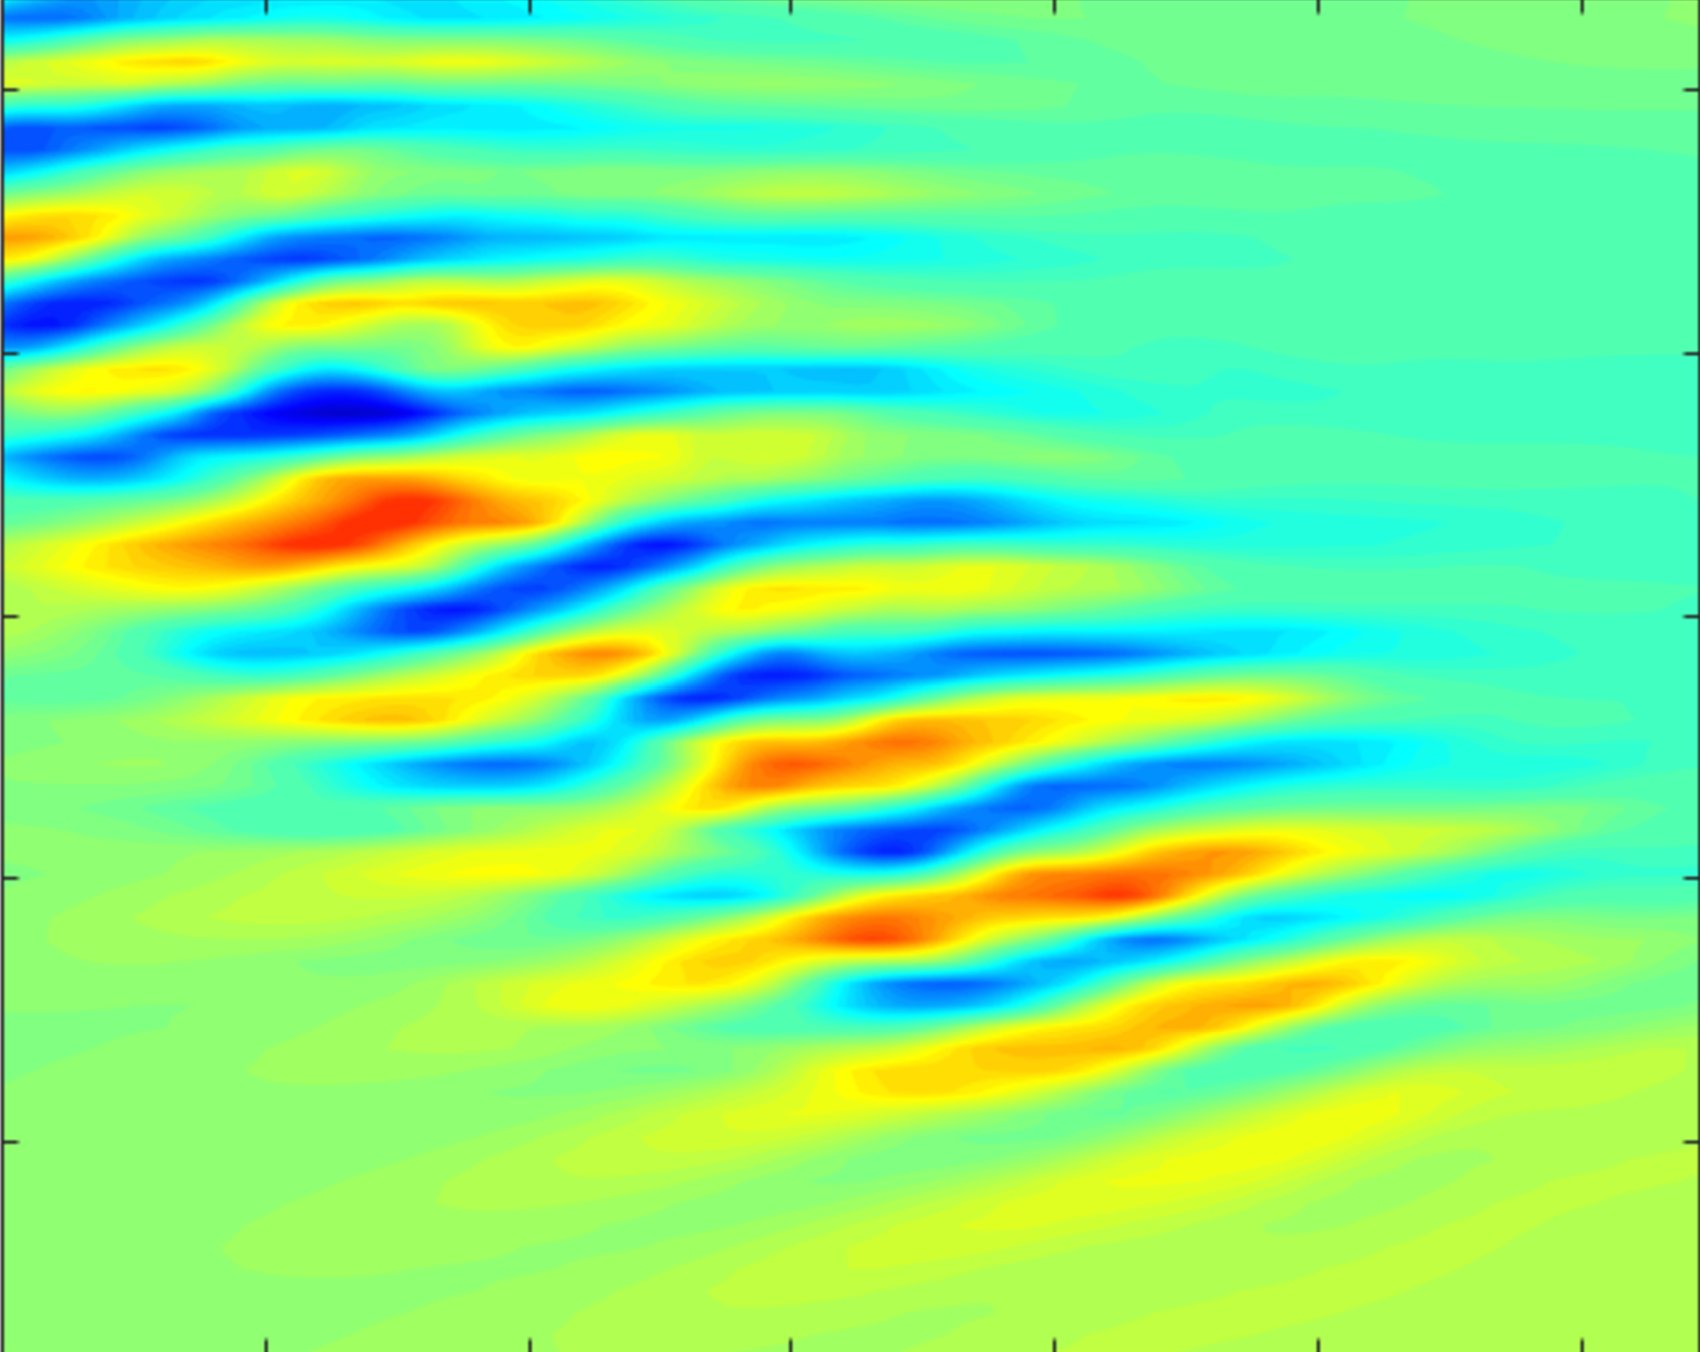
\includegraphics[width = \textwidth]{figures/prediction/actual5300.pdf}}
%	\subfigure[Re=750 t=780.5]{\includegraphics[width = 1\textwidth]{figures/side_wall/bandwall/band750-106-angle.eps}}
	\end{minipage}
	\caption{LSTM预测的后续流场(a-d)与实际流场(e-h)对比。}
\label{fig:lstm_purepred}
\end{figure}

\begin{figure}[H]
	\subfigbottomskip = 2pt
	%\subfigcapskip=-5pt
	\begin{minipage}[h]{\linewidth}
	\centering
	\subfigure{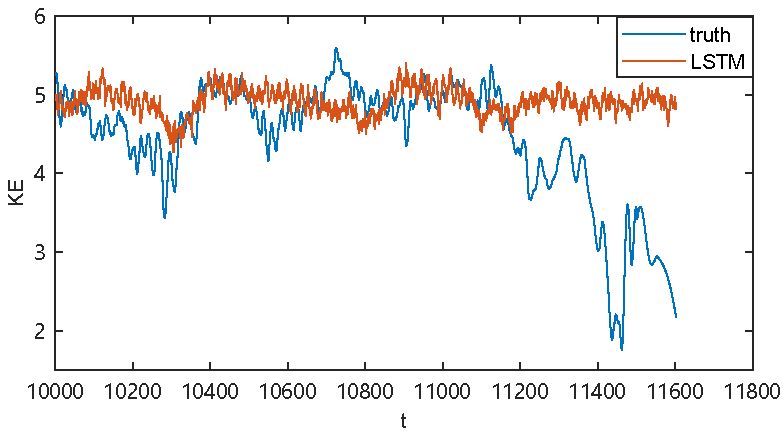
\includegraphics[width = 0.9\textwidth]{figures/prediction/bigwindoweny.pdf}}
	\end{minipage}
	\caption{LSTM预测出的流场能量变化图,以及与实际流场的比较。可以看出在前面的时间段,LSTM预测出的能量在趋势上和实际流场有一定的吻合度,但可以看出在某一时刻后,流场陷入了某个周期稳定解。}
\label{fig:lstm_purepred_eny}
\end{figure}

\subsection{增强数据特征}
通过LSTM的实验结果可以发现,LSTM确实能捕捉到湍流带演化的关键特征,但是无法通过学习到的特征推测出湍流带的瞬态性质。这说明改用更复杂的RNN网络结构对预测任务的表现有明显的提升,因此本文接下来考虑从数据方面着手尝试通过对数据进行适当的预处理进一步提升神经网络预测能力。考虑的方法有三种:1、强调鞍点数据段;2、截断无关数据;3、添加关键物理特征。
\subsubsection{强调鞍点数据}
在Anton的论文中明确指出训练数据中应当包括一个十分接近衰减的数据,否则神经网络完全无法预测MFE流动的最终衰减。因此本文猜测前面神经网络无法预测到湍流带衰减的原因是数据中接近衰减的时间段数据不足,且由于大部分时候都是湍流带稳定存在的数据,因此大量的稳态数据影响了神经网络去专注于表现湍流带瞬态性的数据段。故考虑适当减少湍流带的湍流带数据集的长度,适当的提升湍流带接近衰减的时间段数据的比重。本文截取了后半部分的4600帧作为整体数据集,取前面75\%即3300帧湍流流场作为训练数据集,后面为层流化过程作为验证。从其它使用LSTM预测更复杂流体现象的研究来看,4600帧这个量级的数据可以使得神经网络学到有意义的动力学过程。另外通过头部展向运动速度变化图看出选定的训练数据集中包括了两段头部展向速度明显下降的数据(如图\ref{fig:short_speed}),且其在训练集中的占比相较之前更高。
\begin{figure}[H]
	\subfigbottomskip = 2pt
	%\subfigcapskip=-5pt
	\begin{minipage}[h]{\linewidth}
	\centering
	\subfigure{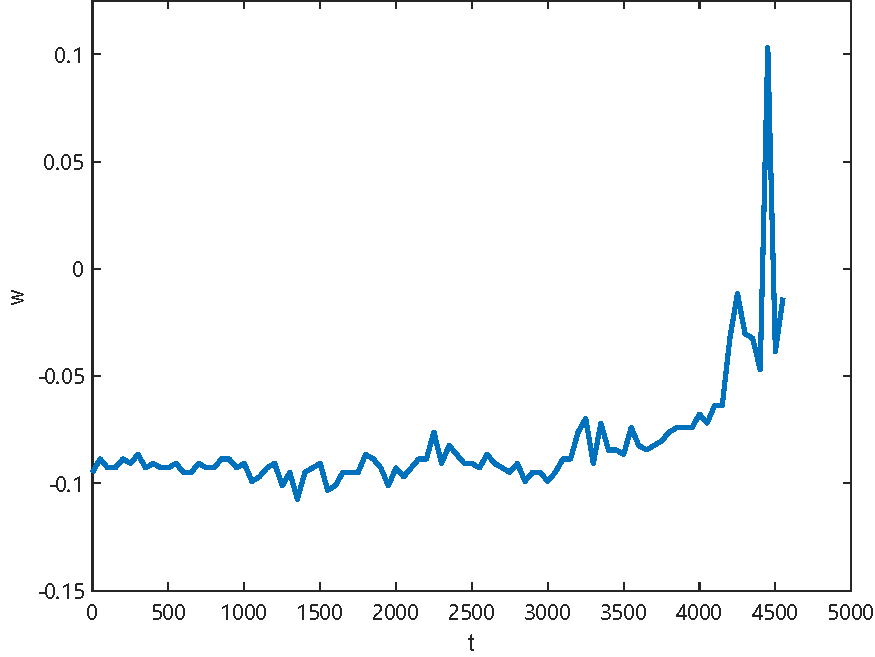
\includegraphics[width = 0.9\textwidth]{figures/prediction/short_speed.pdf}}
	\end{minipage}
	\caption{原始数据集中截取的后4600步数据集,框选的时间段为训练数据集。圆圈选中的时间段中,展向运动速度w有一个明显的下降,且由于整体时间长度的减小,运动速度突变的数据段整体占比升高。}
\label{fig:short_speed}
\end{figure}
\subsubsection{截断尾部波状结构}
前面章节中仅舍弃了流场中的层流区域保留了湍流带主要存在的区域,核心思想是让神经网络专注于更关键的湍流区域。注意到在低雷诺数下,湍流带尾部和中部的大量波状结构其实并不是湍流带自持的关键要素。故考虑对流场数据的区域进一步裁剪,只保留湍流带的头部流场数据,让神经网络只关注对自持起决定性作用的头部区域(图\ref{fig:cutcomp})。
\begin{figure}[H]
	\subfigbottomskip = 2pt
	%\subfigcapskip=-5pt
	\begin{minipage}[h]{0.49\linewidth}
	\centering
	\subfigure[完整湍流带流场]{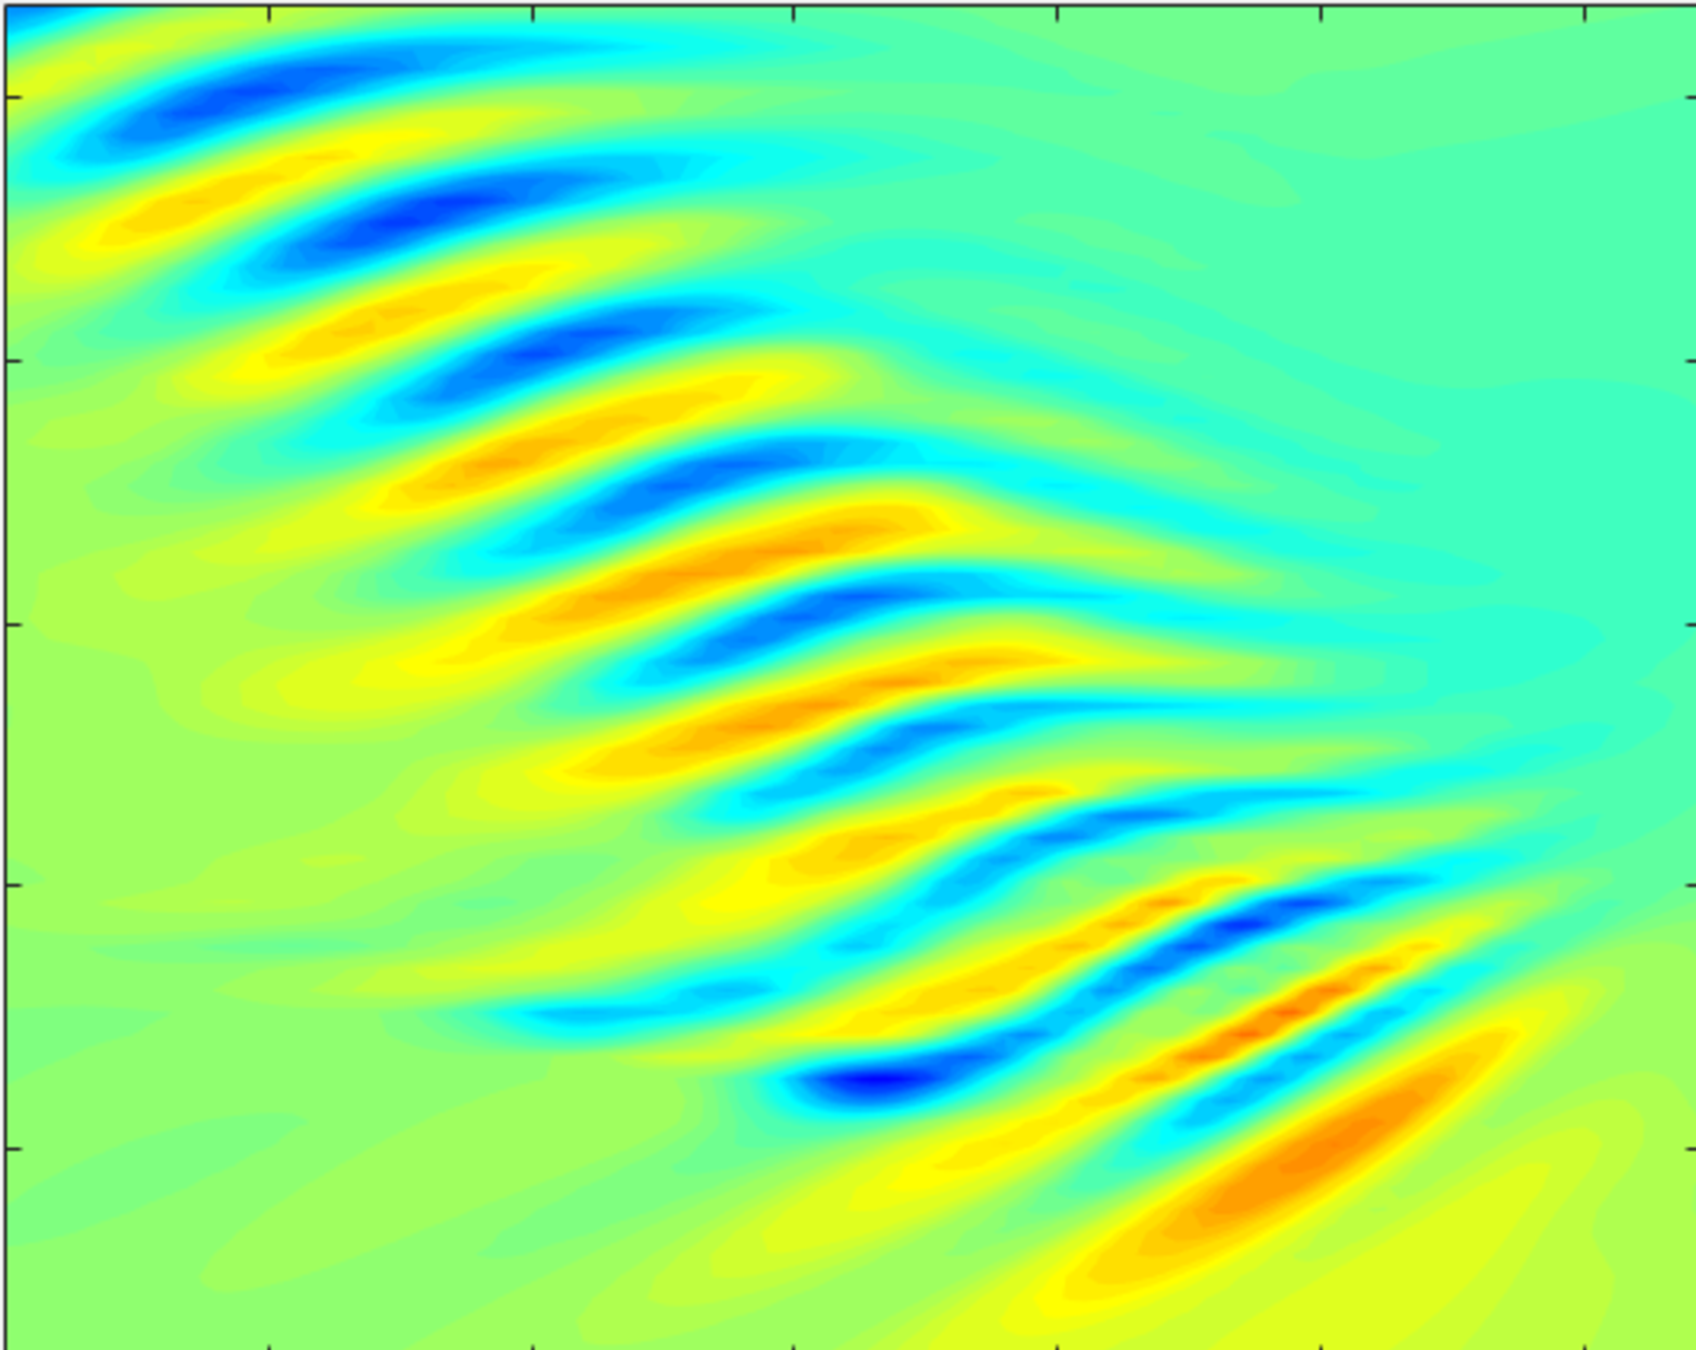
\includegraphics[width = 0.7\textwidth]{figures/prediction/lstm_pure_8000.pdf}}
	\end{minipage}
	\begin{minipage}[h]{0.49\linewidth}
	\centering
	\subfigure[截断尾部波状结构的流场]{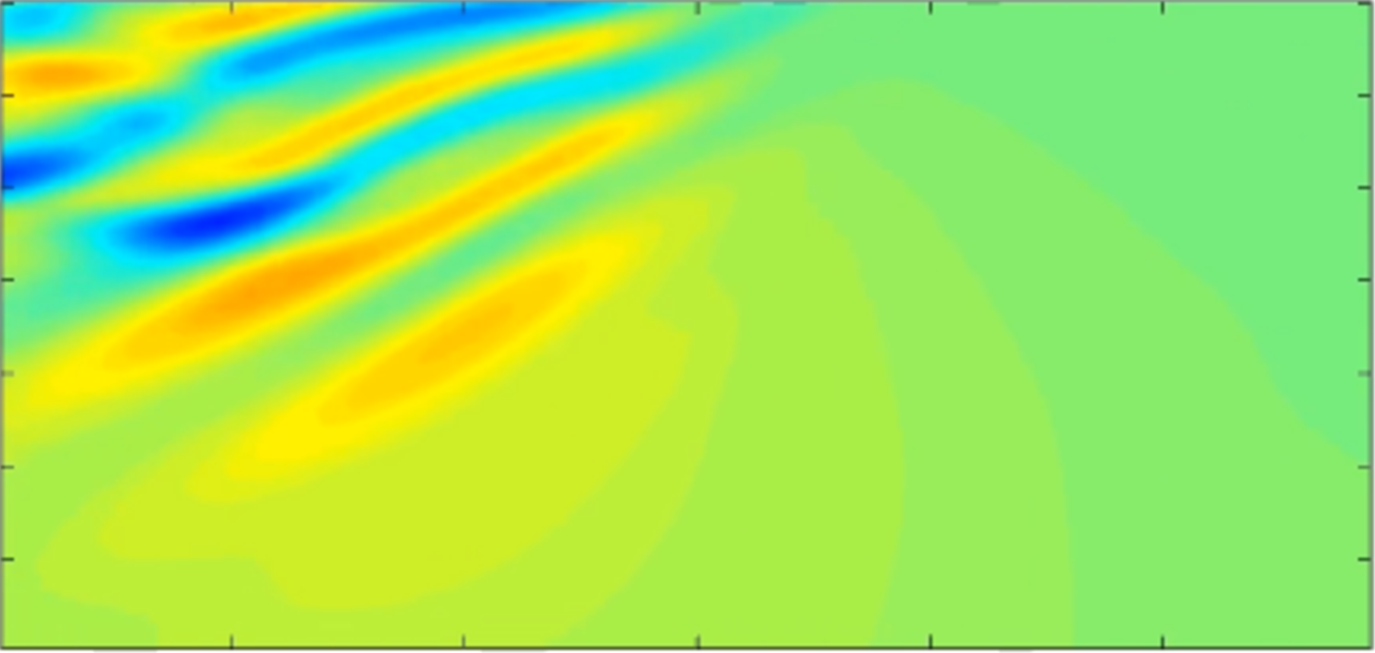
\includegraphics[width = \textwidth]{figures/prediction/truth_511.pdf}}
	\end{minipage}
	
\label{fig:cutcomp}
\end{figure}
\subsubsection{添加头部倾角}
前面LSTM网络的表现证明了神经网络可以捕捉到非线性动力学过程中的固定模式,且能保持重要的物理特征不变,而不能成功预测出湍流带衰减的原因本文猜测是所学习的特征没能表现出明显层流化的趋势,即anton他们提到的训练数据中没有表现出明显的鞍点。故尝试向神经网络提供更直观的特征以提高数据质量。已有研究表明湍流带演化过程中,头部条纹的倾角是头部局地流场不稳定性的一个重要表征,在上一章中指出展向速度型是头部局地不稳定性的主导因素,而头部倾角对展向速度型的缩放十分敏感。因此可以认为头部速度条纹是一个理想的特征,且具有一定的物理可解释性。

关于测量头部条纹的方法,先设置一个统一的阈值,根据该阈值对每一时刻的流场进行二值化,高于阈值的设为1反之则为0(如图\ref{fig:4010angle})。为了防止歧义定义头部条纹为从图中右下往左上捕捉到的第一根足够大的条纹作为代表条纹(排除滤波后极小区域的干扰),其对应的角度(相对于流向)为头部倾角。通过(式\ref{equ:tangle_measure})测量倾角\cite{Tao2017ExtendedLS},其中$x_{i},x{j}$分别代表$x,z$。该算法的基本思路即是用一个最优椭圆去逼近第一根条纹并获得椭圆主轴对应的倾角。

\begin{equation}\label{equ:tangle_measure}
\begin{aligned}
A_{ij} = \frac{\int ex_{i}x_{j} dxdz}{\int e dxdz} - (\frac{\int e x_{i} dxdz}{\int e dxdz})(\frac{\int e x_{i} dxdz}{\int e dxdz})
\end{aligned}
\begin{aligned}
\quad
\theta = \frac{1}{2}arctan(\frac{2A_{xz}}{A_{xx}-A_{zz}})
\end{aligned}
\end{equation}


\begin{figure}[htb]
	\subfigbottomskip = 2pt
	%\subfigcapskip=-5pt
	\begin{minipage}[h]{0.5\linewidth}
	\centering
	\subfigure[]{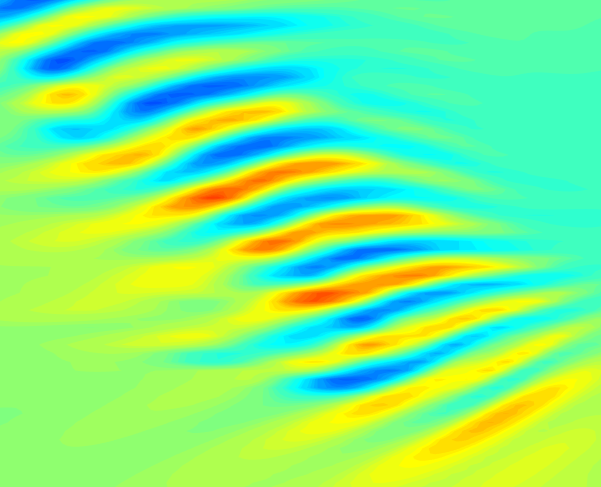
\includegraphics[width = 0.82\textwidth]{figures/prediction/4010.png}}
	\end{minipage}
	\quad
	\subfigbottomskip = 2pt
	%\subfigcapskip=-5pt
	\begin{minipage}[h]{0.5\linewidth}
	\centering
	\subfigure[]{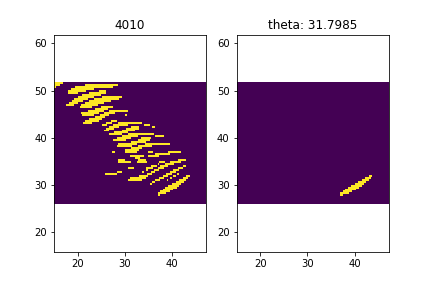
\includegraphics[width = 1\textwidth]{figures/prediction/4010band.png}}
	\end{minipage}
	\quad
	\caption{t=4010时,实际流场(a)与二值化后的流场(b)对比。通过递归法找出所有不连通条带区域,接着挑选出右下第一根面积大于某一阈值的条纹作为代表条纹,测算其倾角。}
\label{fig:4010angle}
\end{figure}

根据以上算法得到关于头部条纹的原始时间序列数据\ref{fig:angle_process}(a),可以看到头部倾角在时间尺度上表现出很强的波动性。这是因为本文并不单纯的选择空间上第一根条纹作为代表,而是要求条纹区域有一定面积,这说明条纹已充分发展了一段时间可以更好的代表头部附近的总体情况。针对原始数据本文用适当的滤波器对获得的原始数据做了时间尺度上的平滑化处理,经过比较本文选择了Savitzky-Golay滤波器,且在多项式阶数为50,窗口帧数为390时获得数据效果最佳(图\ref{fig:angle_process})。
\begin{figure}[H]
	\subfigbottomskip = 2pt
	%\subfigcapskip=-5pt
	\begin{minipage}[h]{\linewidth}
	\centering
	\subfigure[原始取样倾角与滤波后数据]{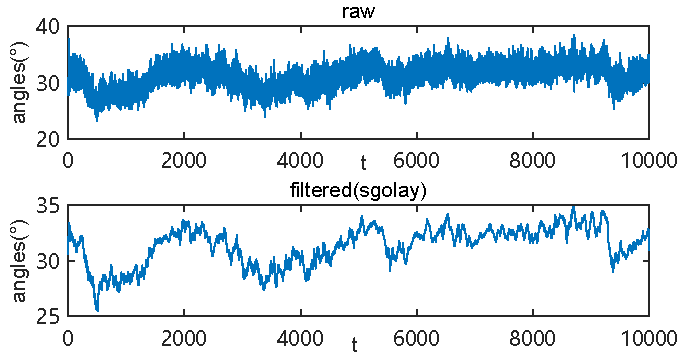
\includegraphics[width = 0.72\textwidth]{figures/prediction/filteredangle.pdf}}
	\end{minipage}
	\quad
	\begin{minipage}[h]{1\linewidth}
	\centering
	\subfigure[头部倾角与头部展向运动速度变化对比]{\includegraphics[width = 0.75\textwidth]{figures/prediction/anglecomp.pdf}}
	\end{minipage}
	\quad
	\caption{头部倾角随时间变化的数据。(a)上图为取样得到的原始倾角数据,下图代表经过滤波在时间尺度上平滑化后的数据。(b)头部倾角变化与展向运动速度变化的对比。可以看出,在展向流速突然减小的同时(图中阴影部分)都能观察到头部倾角大幅度下降的现象。}
\label{fig:angle_process}
\end{figure}

与展向运动速度变化作对比\ref{fig:angle_process}(b),在展向速度大小突然减小的区间可以相应地观察到头部条纹角度的急剧减小;同时在角度急剧减小的区间也能观察到速度大小有减小的趋势。这表明湍流带角度变化与展向速度变化在表征头部不稳定性的能力上是等价的。另外这也表明从角度变化来看,选定的训练数据集中湍流带确实多次靠近了动力学的鞍点结构。从数据粒度上看,湍流带局部移动速度并不是实时测量得到的,是在相隔固定的时间段后间接测量得到的。因此数据粒度较粗且误差较大;而头部条纹角度是每一帧流场实测得到的精确数据,粒度更细且数值精度更高。因此可以认为湍流带角度是一个足够好的额外数据特征。

\subsubsection{增强特征后预测效果}
在增强数据特征后,能量变化曲线上(\ref{fig:LSTM_angle_eny})可以观察到,虽然LSTM仍未能成功预测衰减,但相比起未增强特征的预测结果,流场能量波动更加剧烈,趋向层流化的时刻更多。这可能代表增强特征后湍流带进一步挖掘到动力学中周期成分之外的成分,且有可能学习到了湍流带不能自持的瞬态性质,因此预测的流场能量会比之前更多的趋向于层流化级别的能量大小。
\begin{figure}[H]
	%\subfigcapskip=-5pt
	\begin{minipage}[h]{0.24\linewidth}
	\centering
	\subfigure[LSTM]{\includegraphics[width = \textwidth]{figures/prediction/lstm_angle_100.pdf}}
	\end{minipage}
	%\subfigcapskip=-5pt
	\begin{minipage}[h]{0.24\linewidth}
	\centering
	\subfigure[]{\includegraphics[width = \textwidth]{figures/prediction/lstm_angle_1084.pdf}}
	\end{minipage}
	\begin{minipage}[h]{0.24\linewidth}
	\centering
	\subfigure[]{\includegraphics[width = \textwidth]{figures/prediction/lstm_angle_2631.pdf}}
	\end{minipage}
	\begin{minipage}[h]{0.24\linewidth}
	\centering
	\subfigure[]{\includegraphics[width = \textwidth]{figures/prediction/lstm_angle_3748.pdf}}
	\end{minipage}
	
	\begin{minipage}[h]{0.24\linewidth}
	\centering
	\subfigure[truth]{\includegraphics[width =\textwidth]{figures/prediction/truth_100.pdf}}
	\end{minipage}
	\begin{minipage}[h]{0.24\linewidth}
	\centering
	\subfigure[]{\includegraphics[width = \textwidth]{figures/prediction/truth_511.pdf}}
	\end{minipage}
	\begin{minipage}[h]{0.24\linewidth}
	\centering
	\subfigure[]{\includegraphics[width = \textwidth]{figures/prediction/truth_1062.pdf}}
	\end{minipage}
	\begin{minipage}[h]{0.24\linewidth}
	\centering
	\subfigure[]{\includegraphics[width = \textwidth]{figures/prediction/truth_1520.pdf}}
	\end{minipage}
	\caption{添加头部条纹倾角数据后,LSTM网络的预测表现。本文截取了关键的头部条纹生成部分,舍弃了大部分的波状结构区域以期望神经网络专注于更重要的头部附近。(a)-(d)是LSTM的预测流场,(e)-(h)是实际流场。}
\label{fig:4010angle_performance}
\end{figure}
\begin{figure}[htb]
	%\subfigcapskip=-5pt
	\begin{minipage}[h]{\linewidth}
	\centering
	\subfigure{\includegraphics[width = 0.9\textwidth]{figures/prediction/smallwindoweny.pdf}}
	\end{minipage}
	\quad
	\caption{LSTM预测的流场能量与实际流场能量对比,可以看出与未增强数据特征相比,LSTM预测的流场能量波动更剧烈。}
\label{fig:LSTM_angle_eny}
\end{figure}

\section{小结}
这一章中首先简要介绍了MFE流动的性质以及Anton等采用的神经网络训练方法,并通过适当的修改使其能迁移到湍流带寿命预测的任务上。接着以Re=678情况下的单个湍流带演化至衰减的流场时间序列作为样本数据,验证该训练方法在预测湍流带寿命任务上的可行性,并得到以下结论:

1、Anton所使用的改良ESN方法未能预测出符合力学特性的衰减过程,因此该方法虽然预测出了衰减的发生但其结果在物理上不可靠;

2、使用参数更复杂的LSTM进行预测后,虽然神经网络不能预测出湍流带衰减的最终结果(即没有学习到湍流带瞬态的特性)且似乎陷入了某个稳定周期解,但是其预测出的后续演化过程符合大部分重要的力学特性,即LSTM可以正确的捕捉到湍流带演化中的力学特性。结论是改用结构更加复杂的神经网络替换结构简单的ESN能明显提高流场预测的物理可靠性;

3、对数据进行合理的裁剪、增加关键的力学特征后,神经网络预测出的流场虽仍不能顺利衰减但更不易陷入周期解,且流场能量趋于层流化的几率更高。本文推测这可能代表神经网络学习到了更深层次的演化机制,因此预测的流场更容易表现出衰减的特性,即湍流带本质的瞬态性;

综上所述,本文推测Anton的方法具有一定的有效性,然而由于湍流带的流动结构原复杂于可以仅靠9个模态表征的MFE流动,因此使用结构更复杂参数更多的神经网络或许能捕捉到更深层次湍流带的力学特性,进而成功预测出湍流带的衰减(瞬态性)。

%\subsubsection{测试}
%测试四级标题
